Queremos observar que tan bueno es el algoritmo propuesto en la práctica. Para esto realizaremos una serie de tests utilizando las entradas que se utilizaron en el ejercicio 3.
La idea es tratar de encontrar la configuración ideal para que en promedio el algoritmo resuelva la mayoria de los casos eficientemente. Para lograr esto, experimentamos variando distintos parametros para cada entrada y obtener las respectivas conclusiones de los resultados obtenidos.\\
Los parámetros de estudio fueron:

\begin{enumerate}
\item  \textbf{Cantidad de iteraciones}: Tenemos que observar en promedio, cuantas iteraciones conviene tomar para obtener un buen resutado.
\item \textbf{Tenor tabú}: Tenemos que observar que sucede al aumentar el tenor tabú, y hasta cuanto es conveniente hacerlo para obtener un buen resultado.
\item \textbf{Atributos tabú}: Analizar que sucede al tomar como atributos tabú las aristas que cambiaron o las aristas nuevas
\item \textbf{Función de aspiración}: Elegir la solución más tabú o la menos tabú.
\end{enumerate}

Debemos aclarar, que tenor tabú fué establecido en cantidad de pokeparadas mas gimnasios. Este valor puede ser relativamente grande, pero cuanto más grande, más tiempo de resolución es necesario, con lo cual al final no es una cuestion de memoria, si no, una cuestion de tiempo de computos necesaria para correr el algoritmo.
También se trabajó probando diferentes configuraciones de atributos tabú y función de aspiración, obteniendo en todos los casos los mismos resultados, por lo que al final se decidió dejar prefijado el estandar para tabú search que es aristas viejas como atributos tabú y solución menos tabú para la función de aspiración.\\

Se tomaron 20 mediciones por cada tipo de test y se tomó una media alfa podada de las mismas con $\alpha$ = 0.5 de manera de podar un 25\% de los datos a cada lado.  De esta forma se reduce la posibilidad de outliers en las muestras consideradas.

Como fue enunciado en incisos anteriores de este trabajo las 4 familias en las que la heur\'istica golosa no otorga una soluci\'on \'optima son:

\begin{enumerate}
\item Familia 4
\item Familia 6
\item Familia 7
\item Familia 8
\end{enumerate}

Estas ser\'an las únicas a ser a analizadas, ya que el resto son el resultado exacto o no tienen soluci\'on, con lo cual no aportan mayor relevancia.
 
\subsubsection*{Familia 4}

Veamos algunos resultados de aplicar cada version de tabú search:

\vspace*{0.3cm} \vspace*{0.3cm}
  \begin{center}
 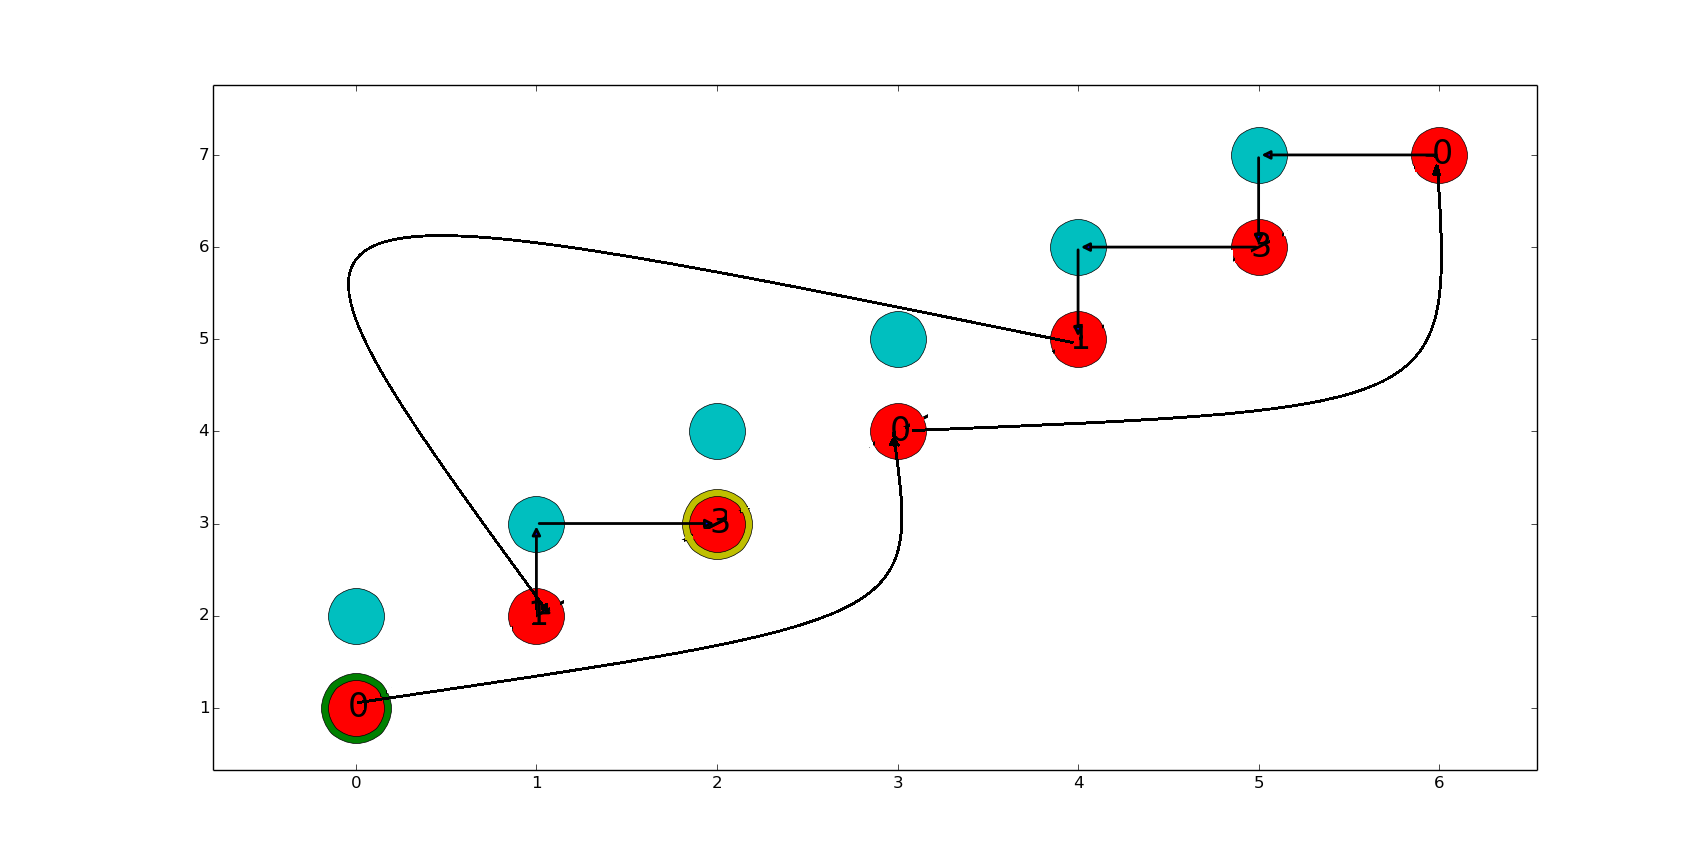
\includegraphics[scale=0.3]{./EJ4/fam4goloso.png}\\
 {            \textit{Soluci\'on Golosa}}
  \end{center}
  \vspace*{0.3cm}

\vspace*{0.3cm} \vspace*{0.3cm}
  \begin{center}
 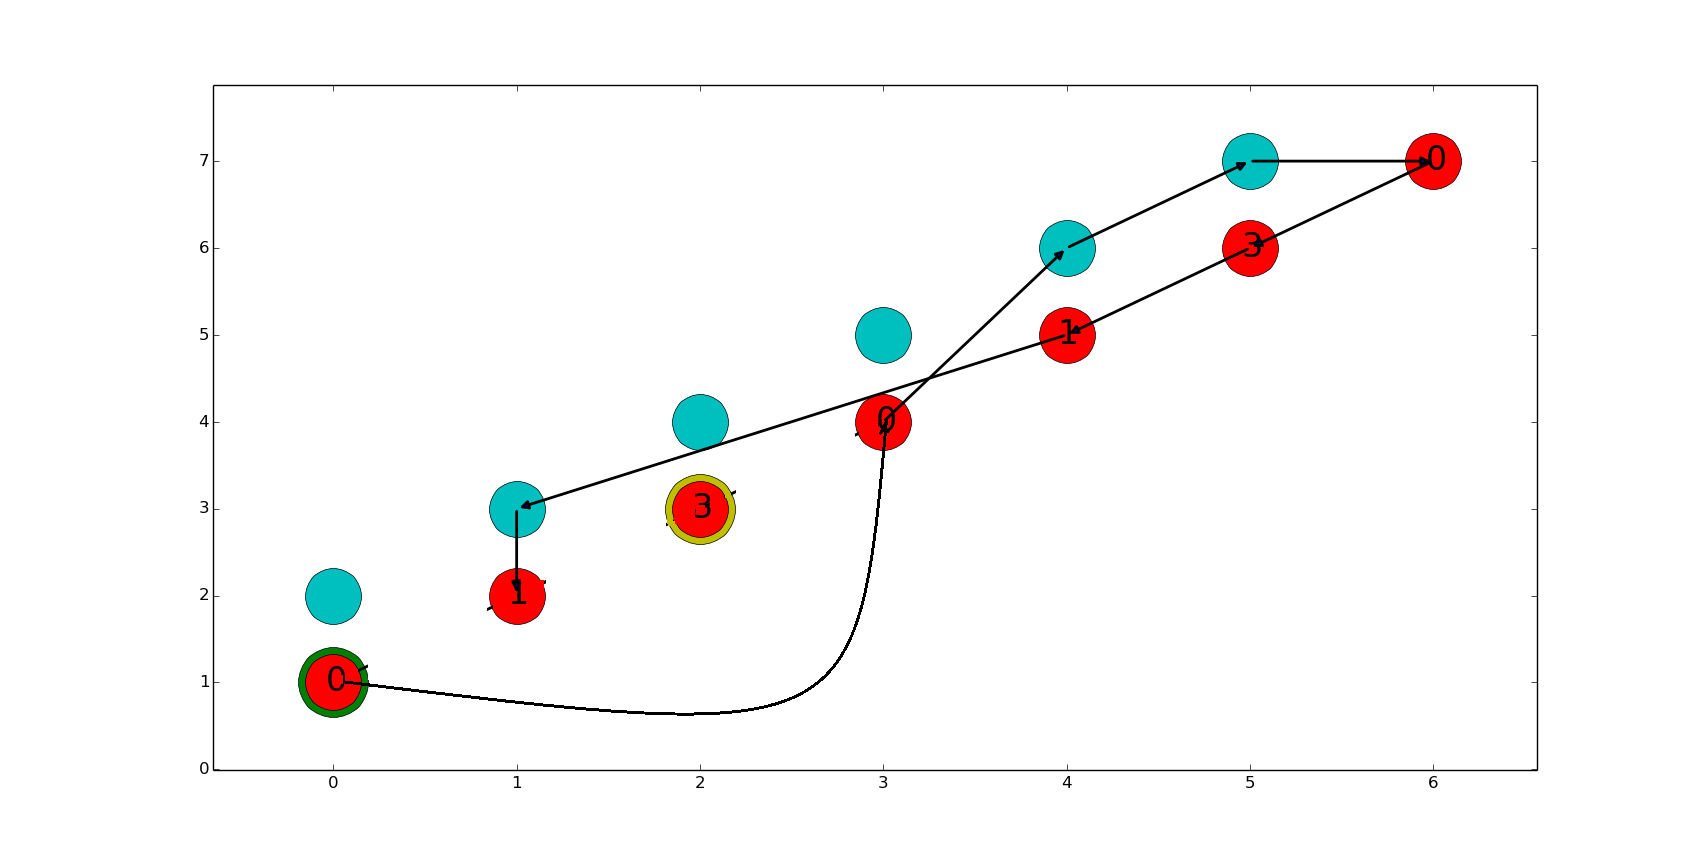
\includegraphics[scale=0.3]{./EJ4/fam42opt.png}\\
 {            \textit{Soluci\'on 2-OPT}}
  \end{center}
  \vspace*{0.3cm}

\vspace*{0.3cm} \vspace*{0.3cm}
  \begin{center}
 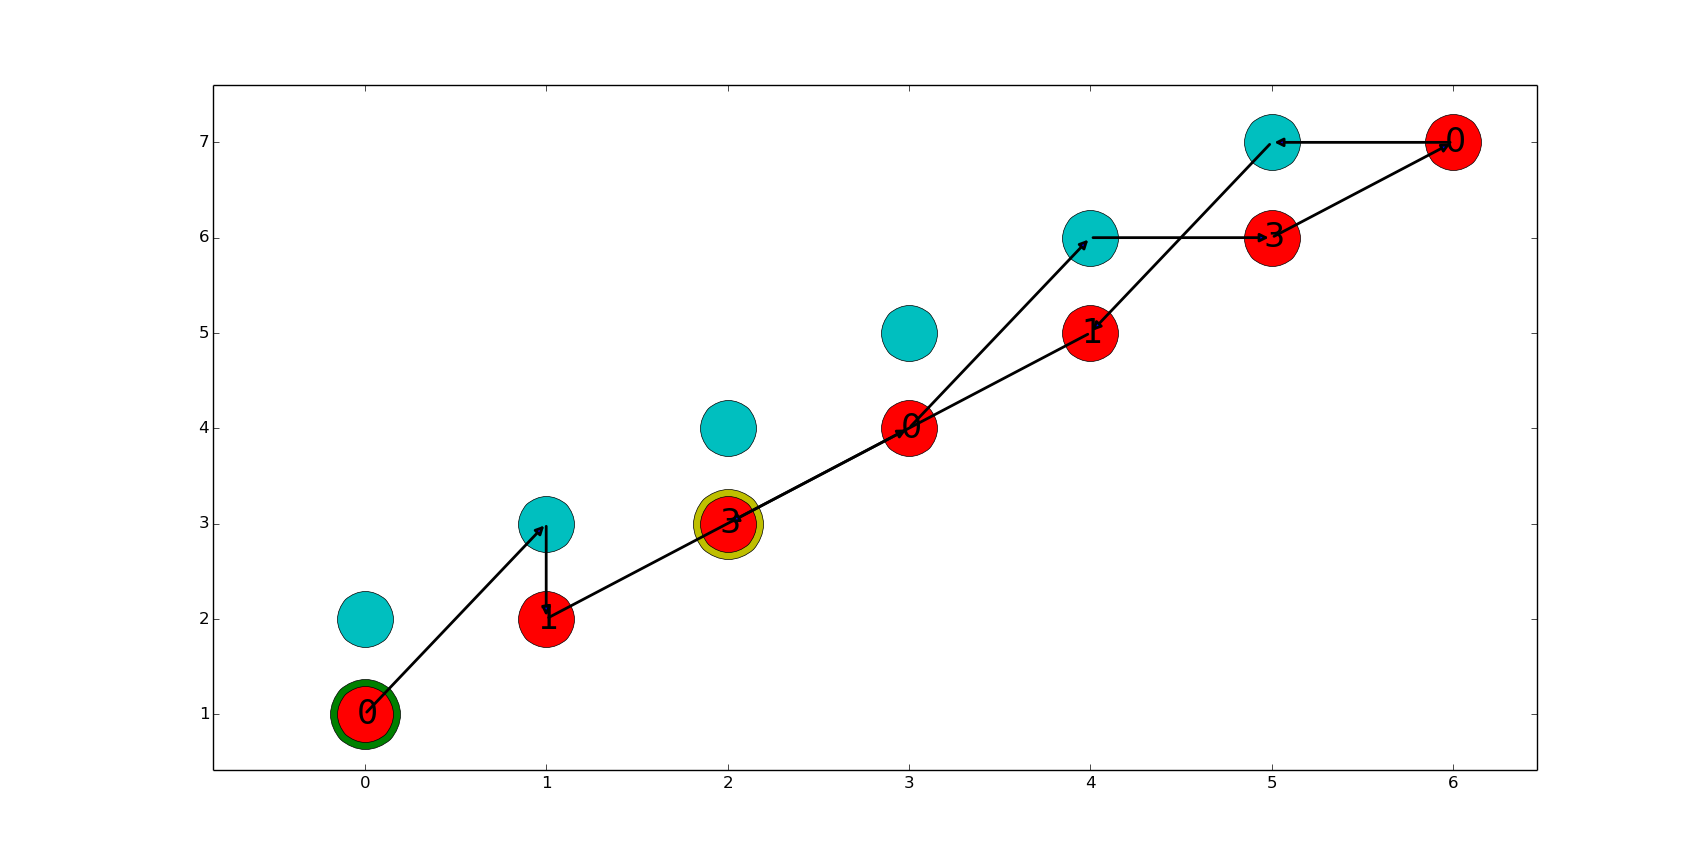
\includegraphics[scale=0.3]{./EJ4/fam43opt.png}\\
 {            \textit{Soluci\'on 3-OPT}}
  \end{center}
  \vspace*{0.3cm}

Nos parece interente comparar los resultados de mejora y tiempo de las búsquedas locales y tabú search que utilicen la misma vecindad, para ver si tabú search mejora lo logrado por la búsqueda local o empeora el resultado. Esto será realizado para cada familia mencionada.\\

Veamos como se comporta tabú 2-OPT con respecto a la heuristica de búsqueda local 2-OPT dentro de la familia 4:

\vspace*{0.3cm} \vspace*{0.3cm}
  \begin{center}
 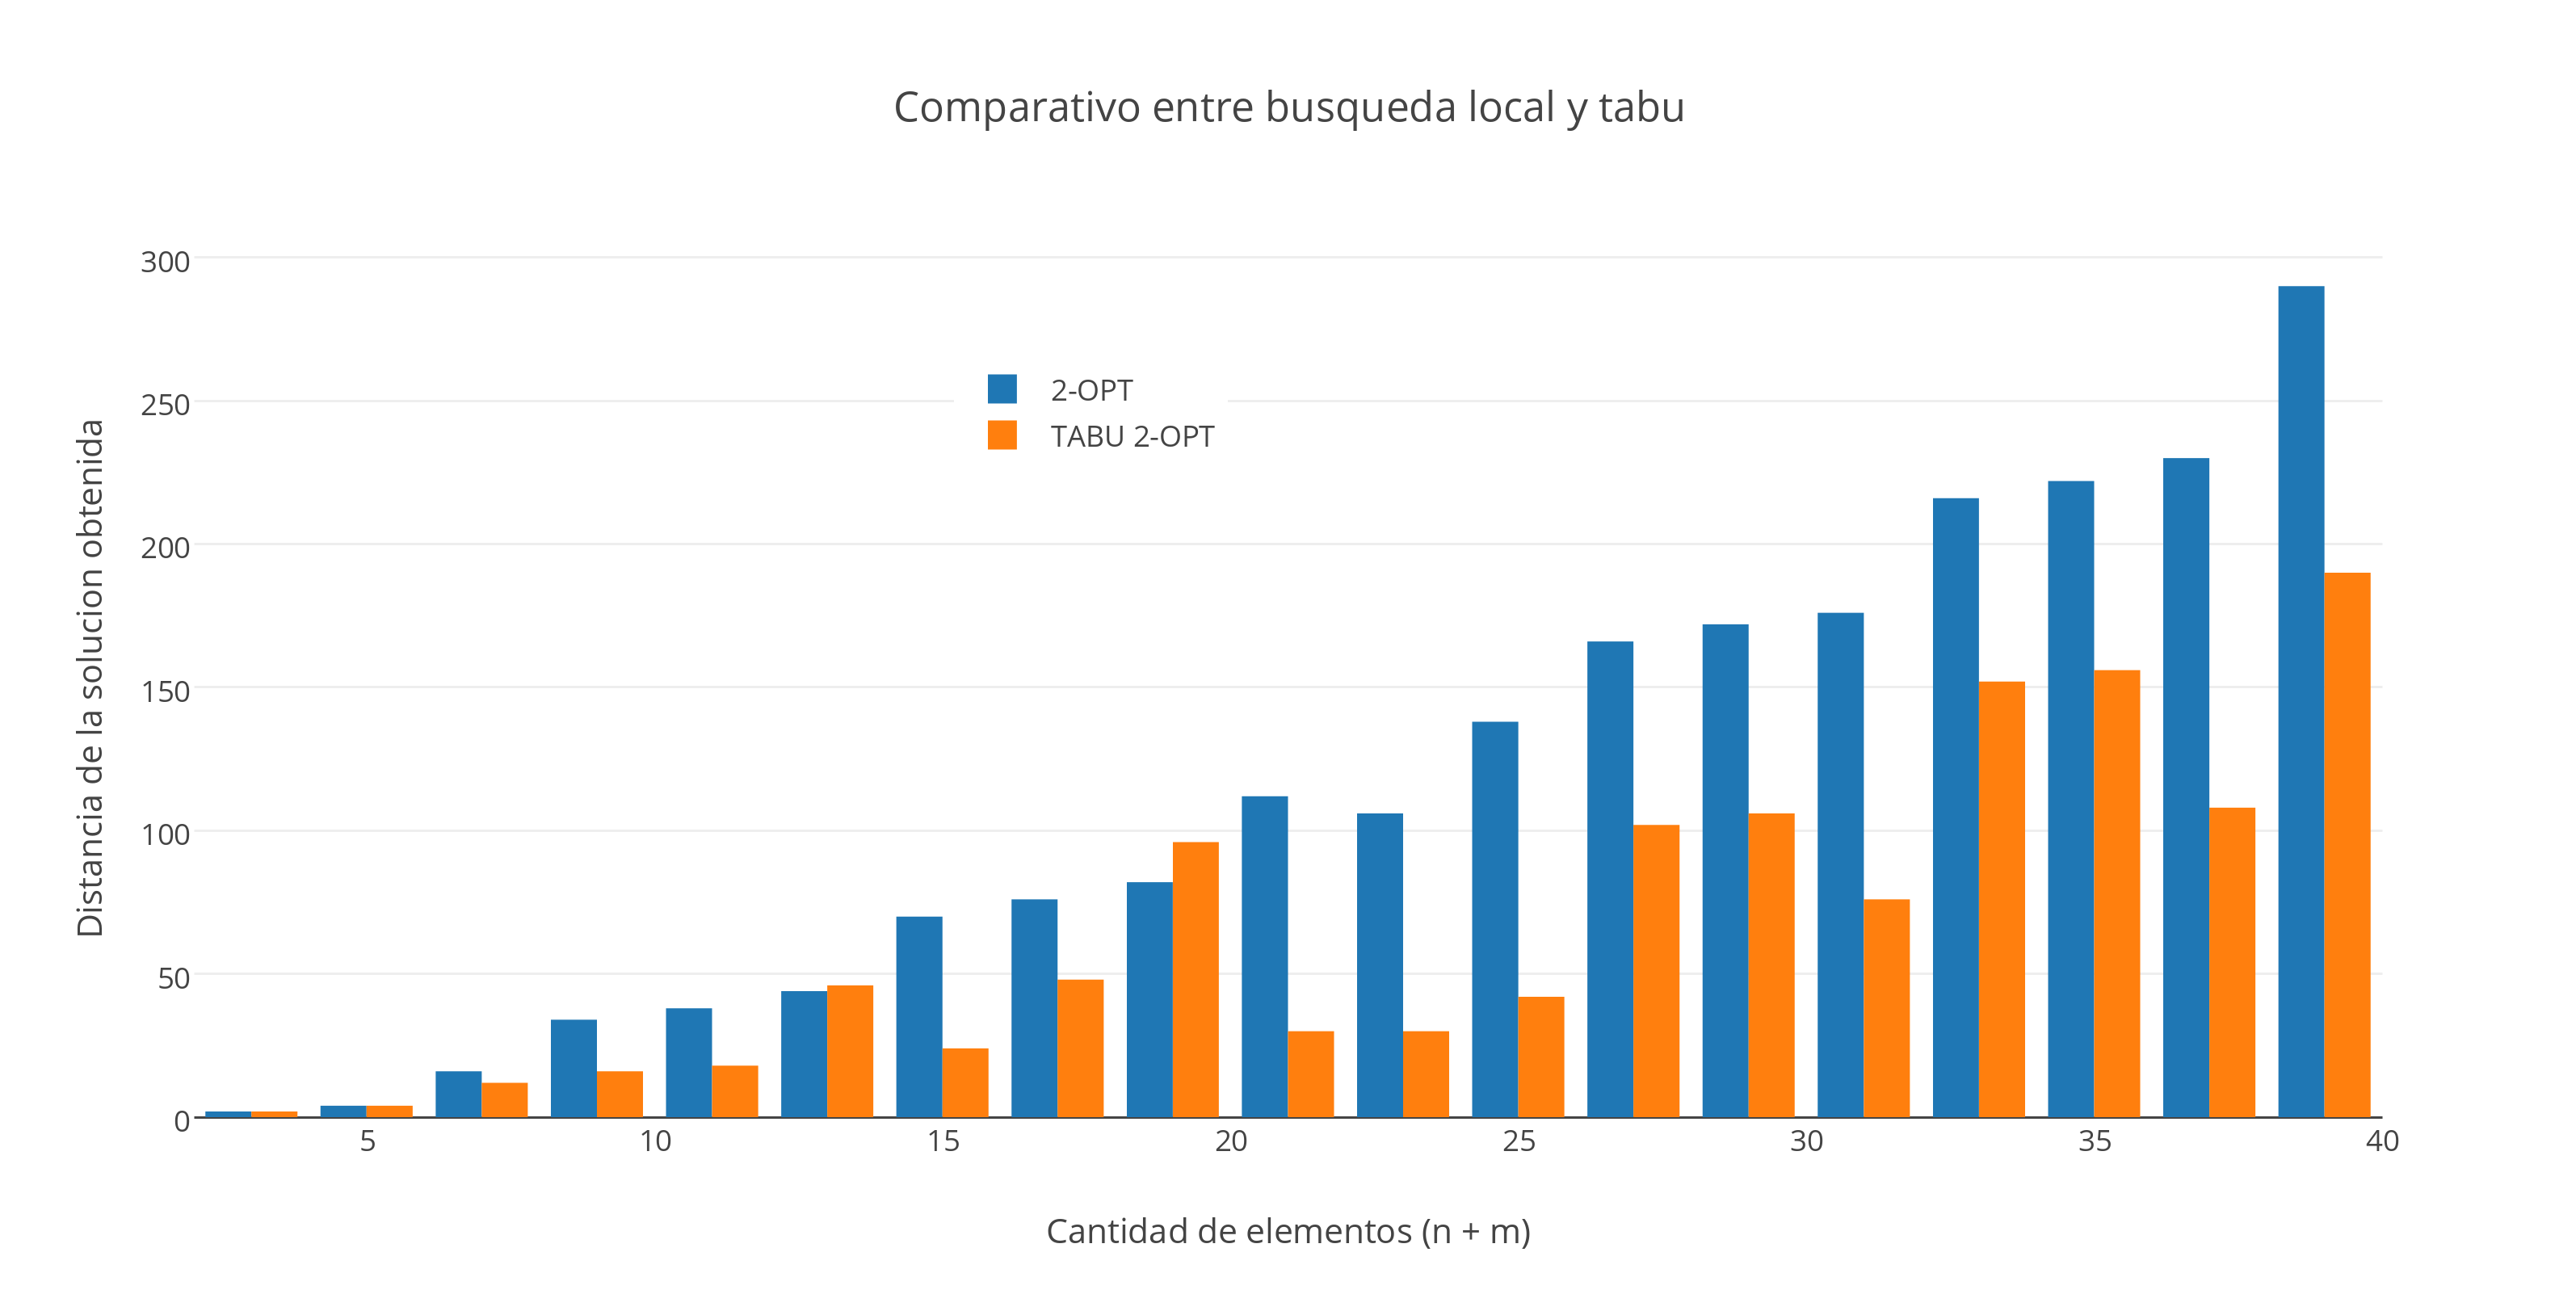
\includegraphics[scale=0.5]{./EJ4/comparativogym02opt.png}\\
 {            \textit{Gráfico \ 4.1 - 2-OPT vs Tabu 2-OPT sobre Familia 4}}
  \end{center}
  \vspace*{0.3cm}

En cuanto a tiempo insumido vemos lo siguiente:

\vspace*{0.3cm} \vspace*{0.3cm}
  \begin{center}
 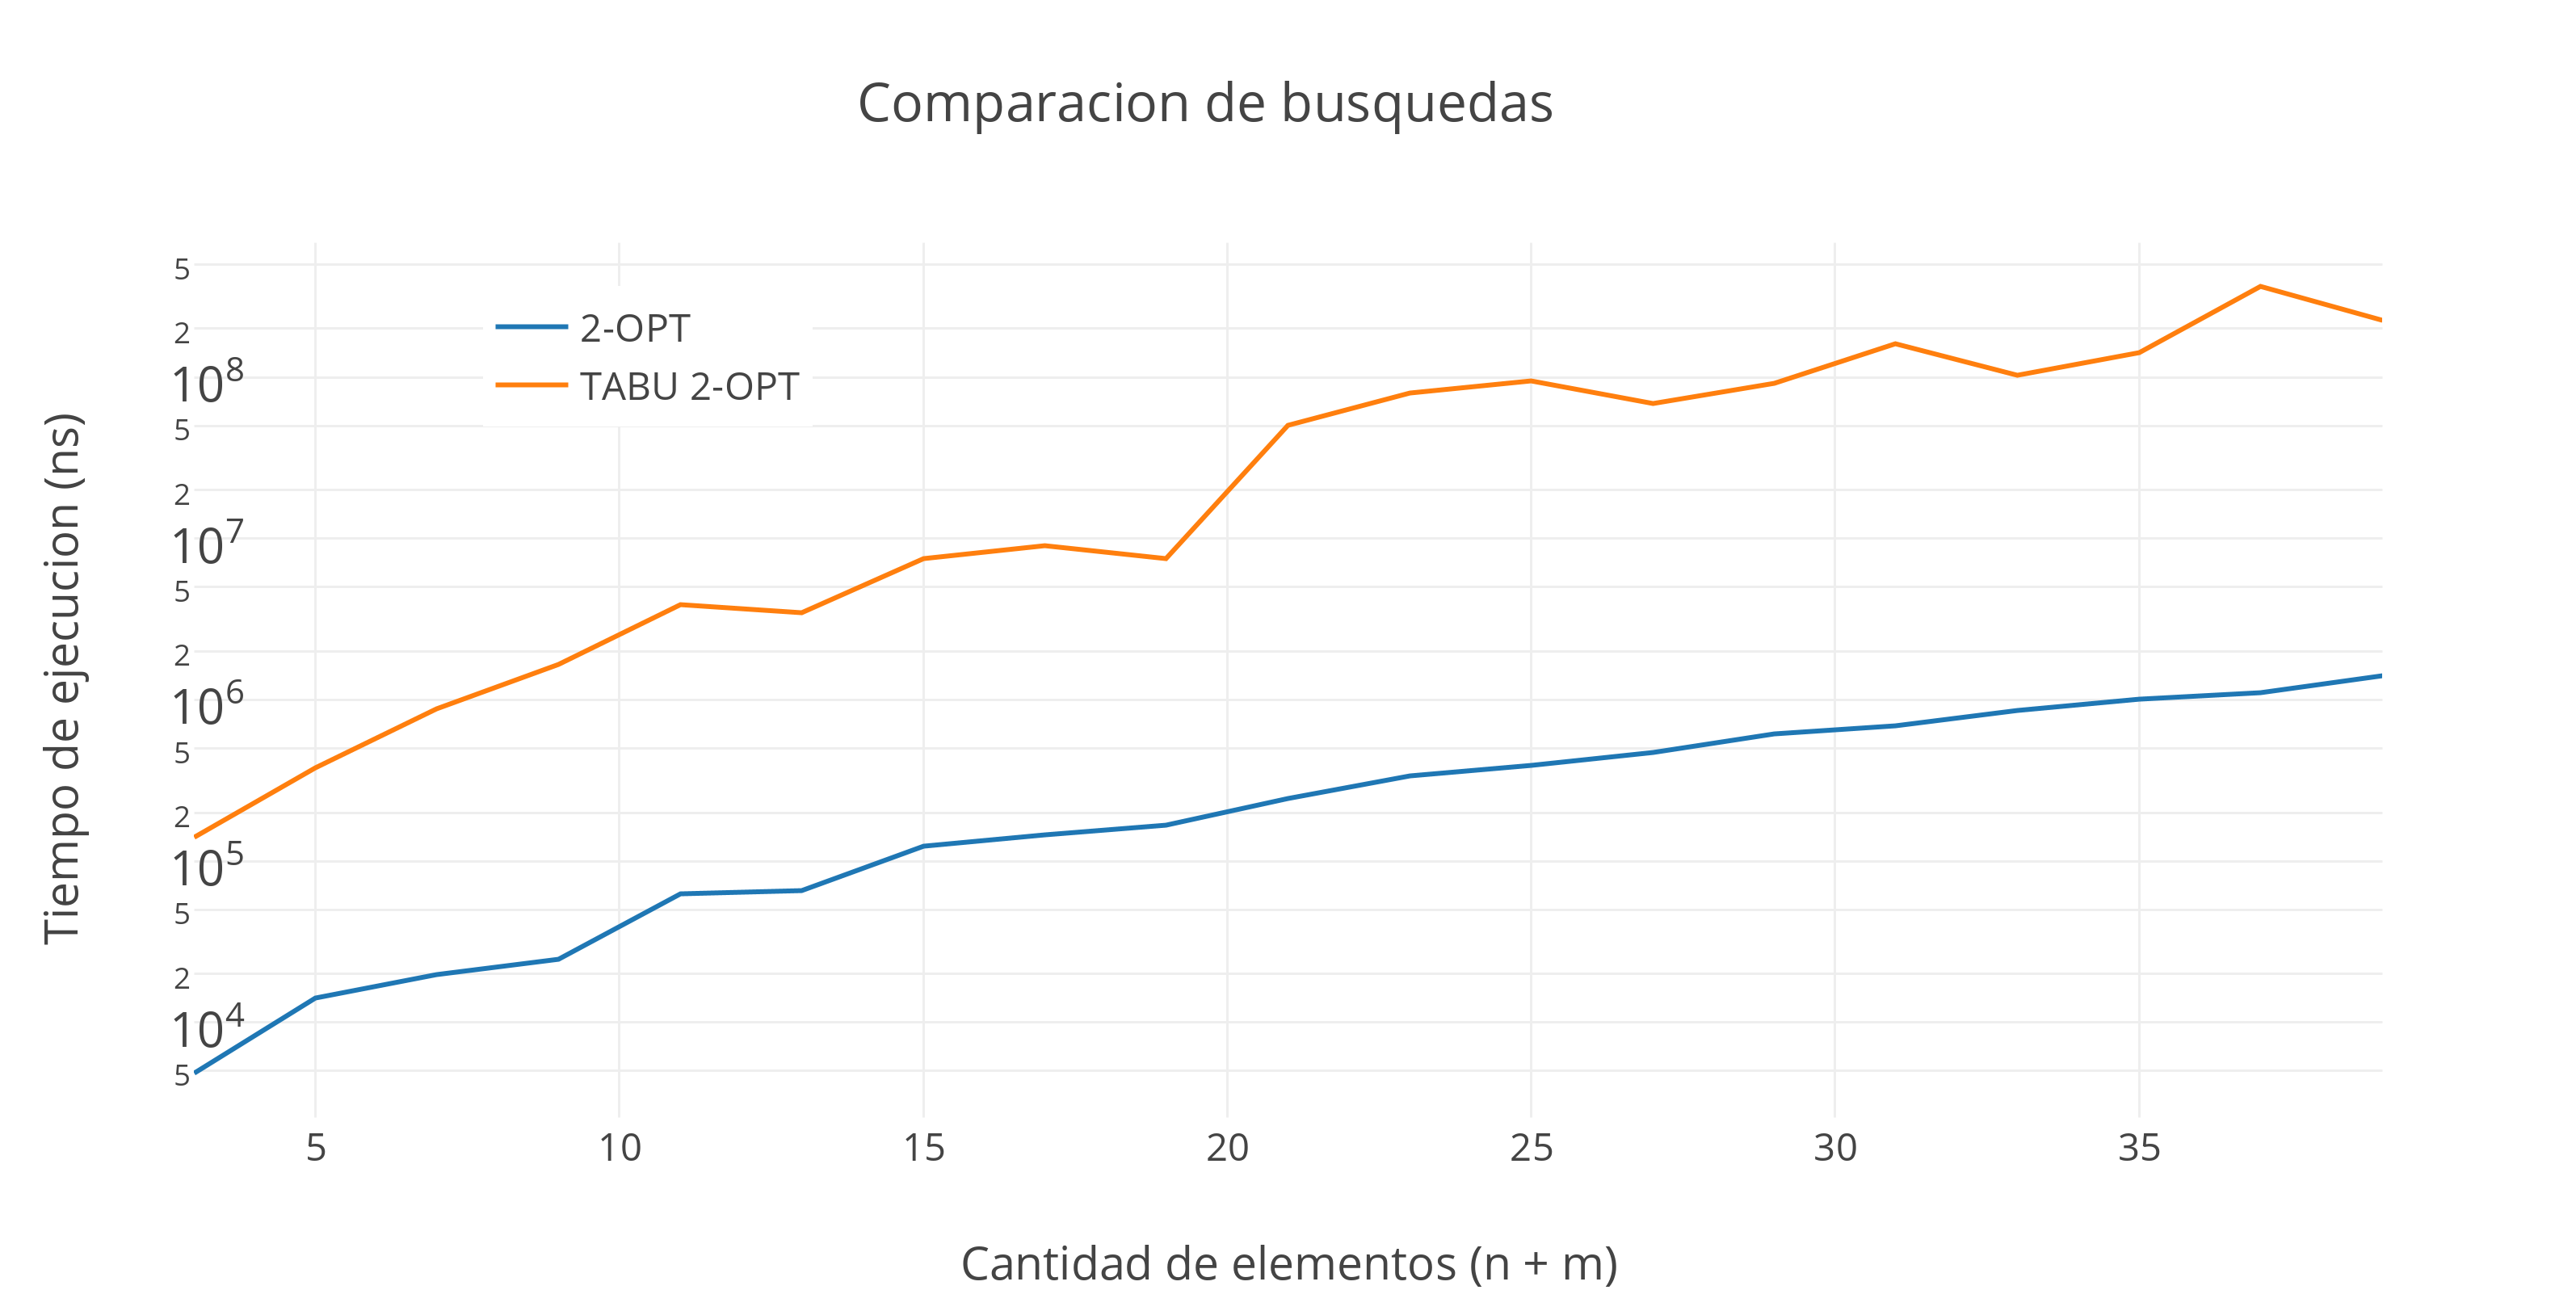
\includegraphics[scale=0.5]{./EJ4/medicion2optgym0.png}\\
 {            \textit{Gráfico \ 4.2 - 2-OPT vs Tabu 2-OPT sobre Familia 4}}
  \end{center}
  \vspace*{0.3cm}
  
 Aplicando 3-OPT:

\vspace*{0.3cm} \vspace*{0.3cm}
  \begin{center}
 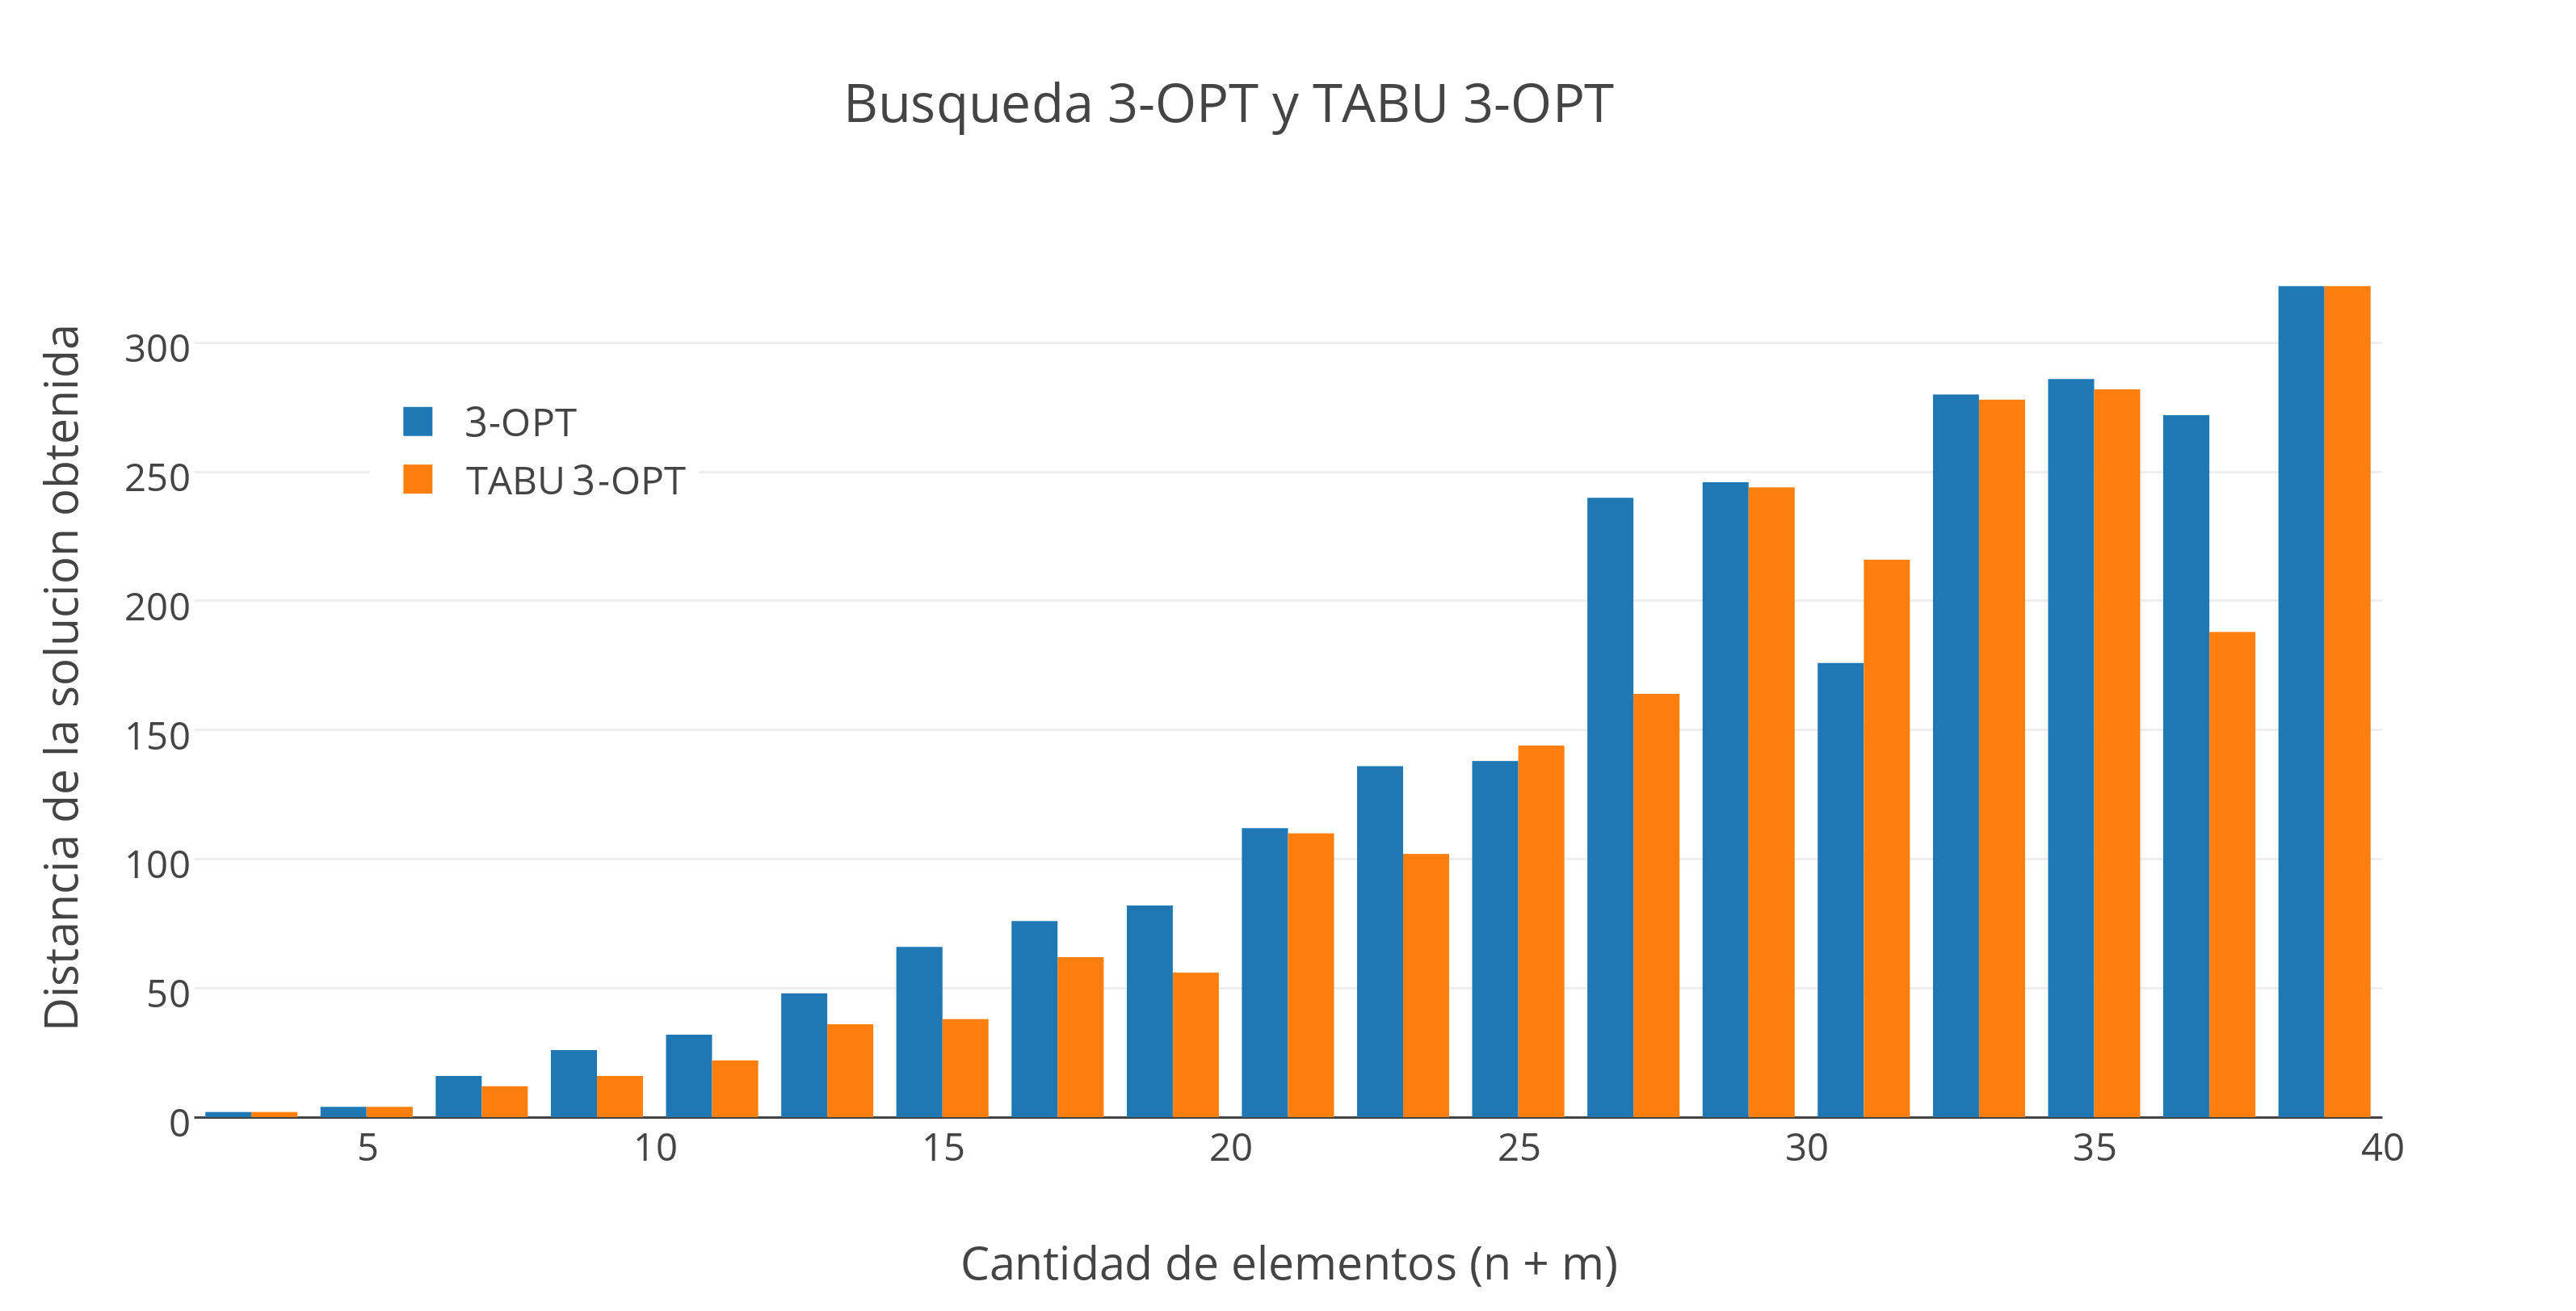
\includegraphics[scale=0.5]{./EJ4/comparativogym03opt.png}\\
 {            \textit{Gráfico \ 4.3 - 3-OPT vs Tabu 3-OPT sobre Familia 4}}
  \end{center}
  \vspace*{0.3cm}

\vspace*{0.3cm} \vspace*{0.3cm}
  \begin{center}
 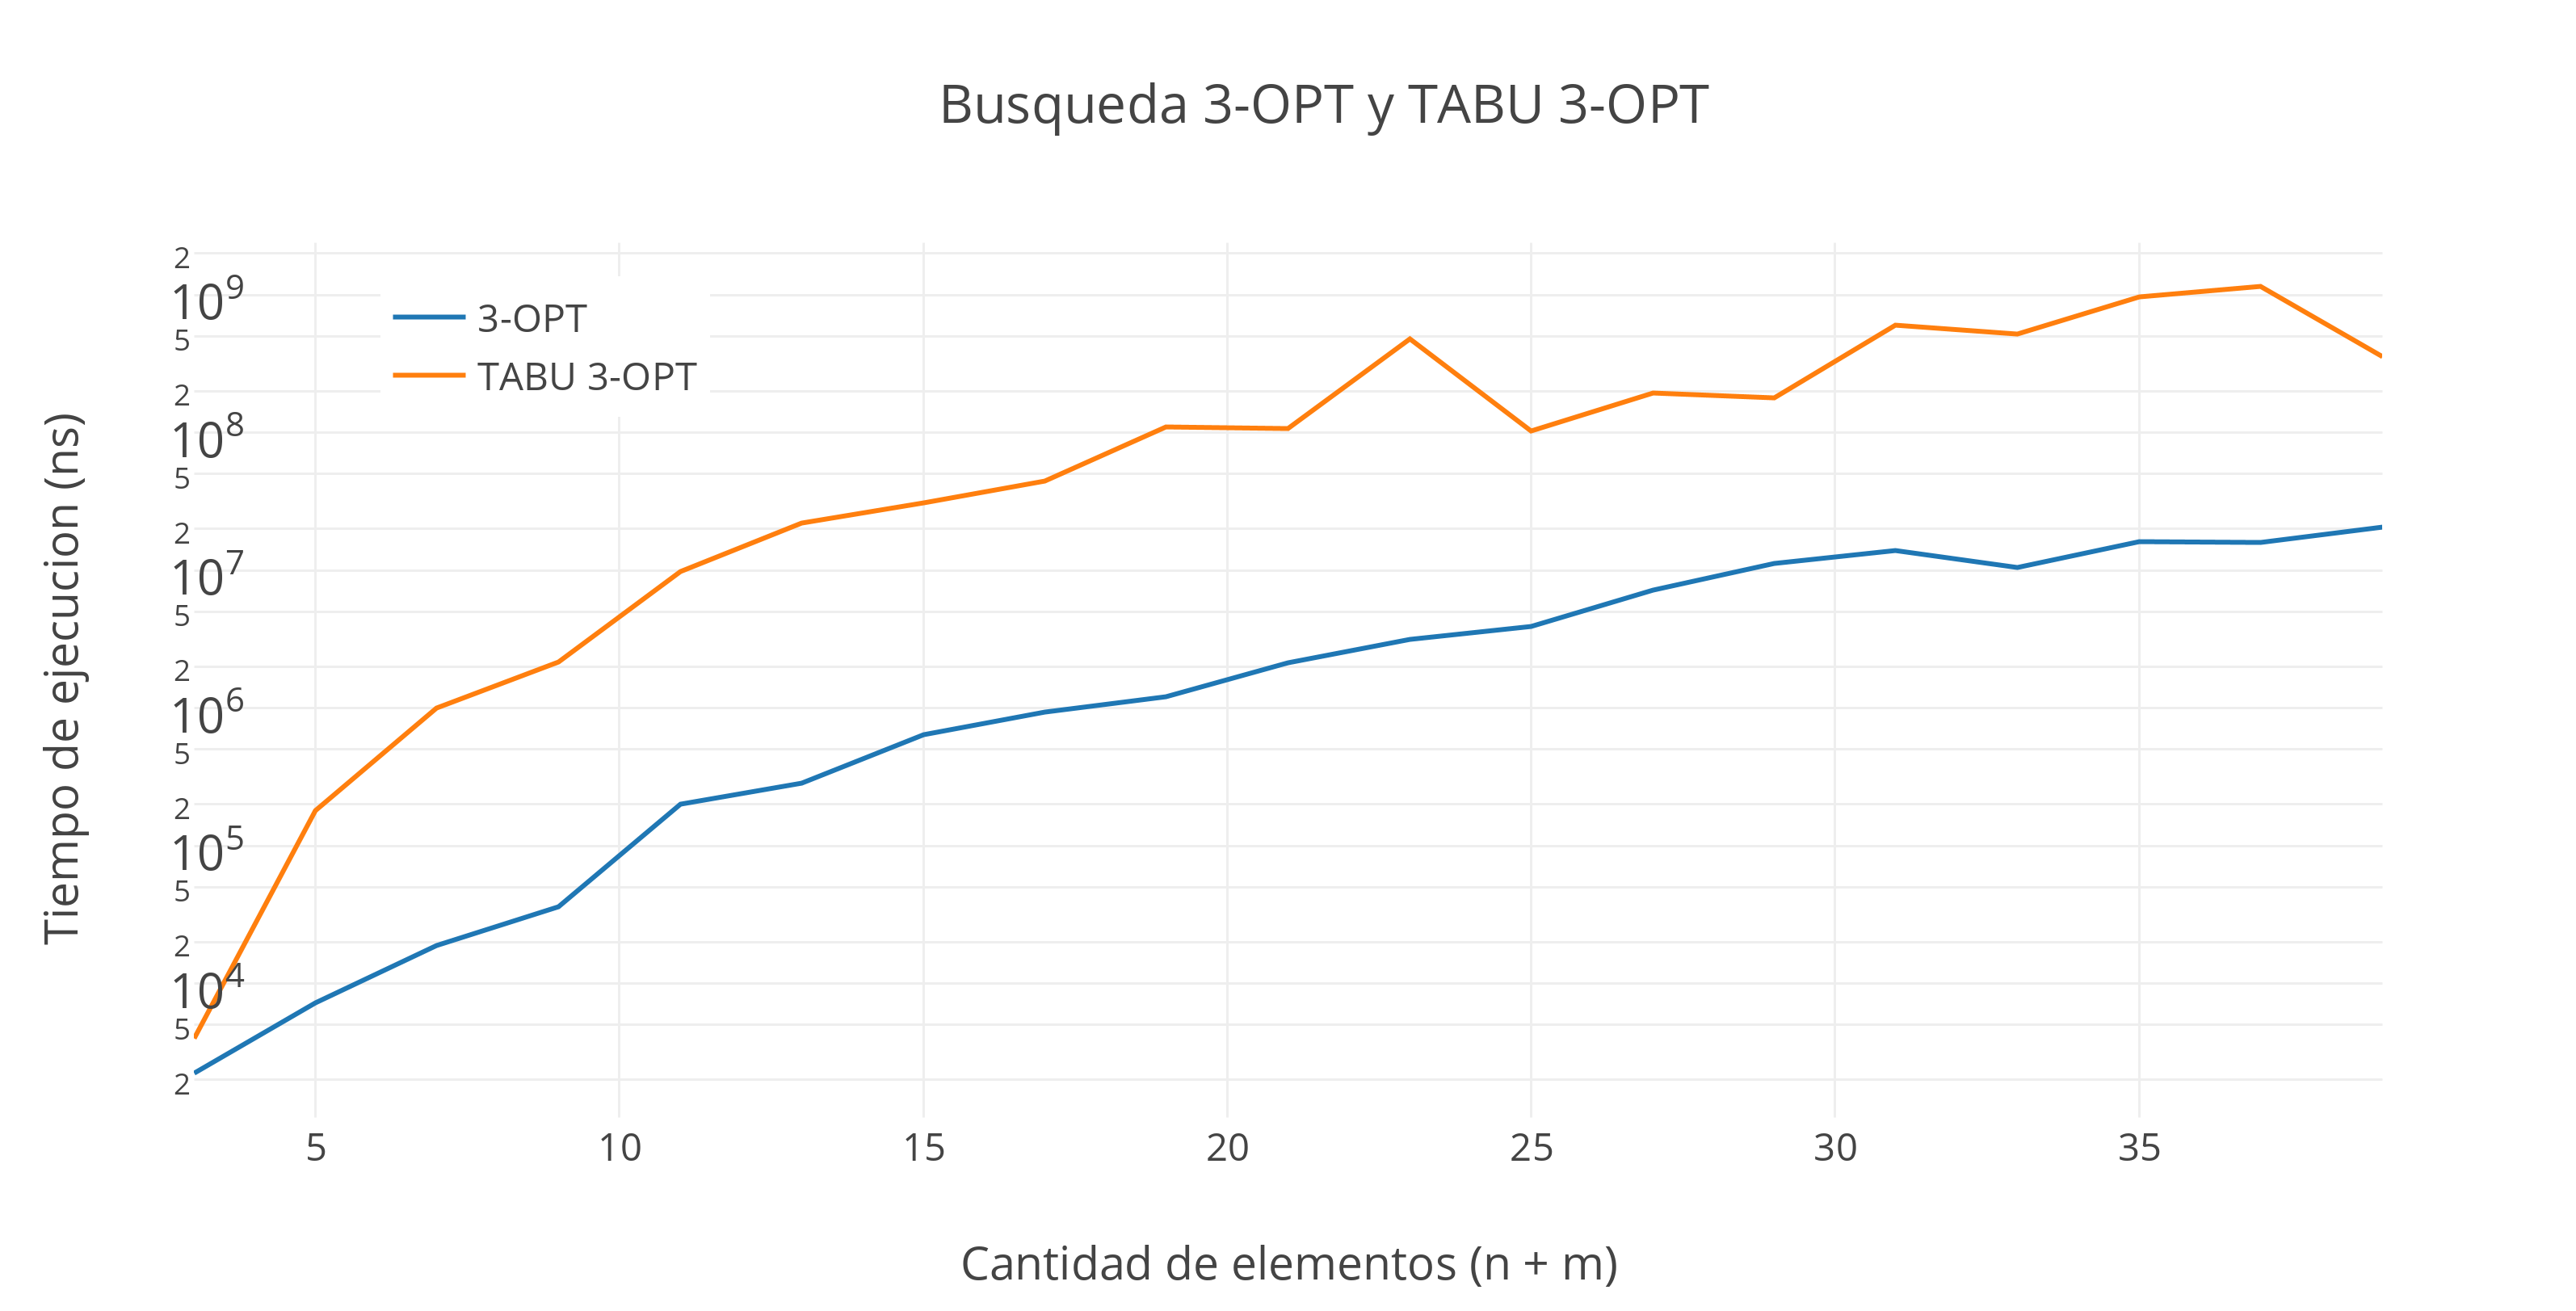
\includegraphics[scale=0.5]{./EJ4/medicion3optgym0.png}\\
 {            \textit{Gráfico \ 4.4 - 3-OPT vs Tabu 3-OPT sobre Familia 4}}
  \end{center}
  \vspace*{0.3cm}
  
Podemos observar que tabú search 2-OPT mejora lo realizado por la heuristica de búsqueda local 2-OPT. Los tiempos insumidos para lograrlo son elevados, pero en relación a la mejora es un resultado aceptable en la práctica. No así tabú search 3-OPT que apenas mejora lo realizado por búsqueda local 3-OPT y requiere tiempos elevados de corrida del algoritmo.\\
  
Para decidir que vecindad es mejor utilizar en tabú search, se comparará conjuntamente el tiempo de ejecución con la calidad de la solución. Para esta última tendremos en cuenta que los algoritmos, de devolver un resultado, serán válidos: esto quiere decir que cuanto menor distancia recorran las soluciones, mejor serán las mismas:

Las soluciones obtenidas fueron las siguientes:

\vspace*{0.3cm} \vspace*{0.3cm}
  \begin{center}
 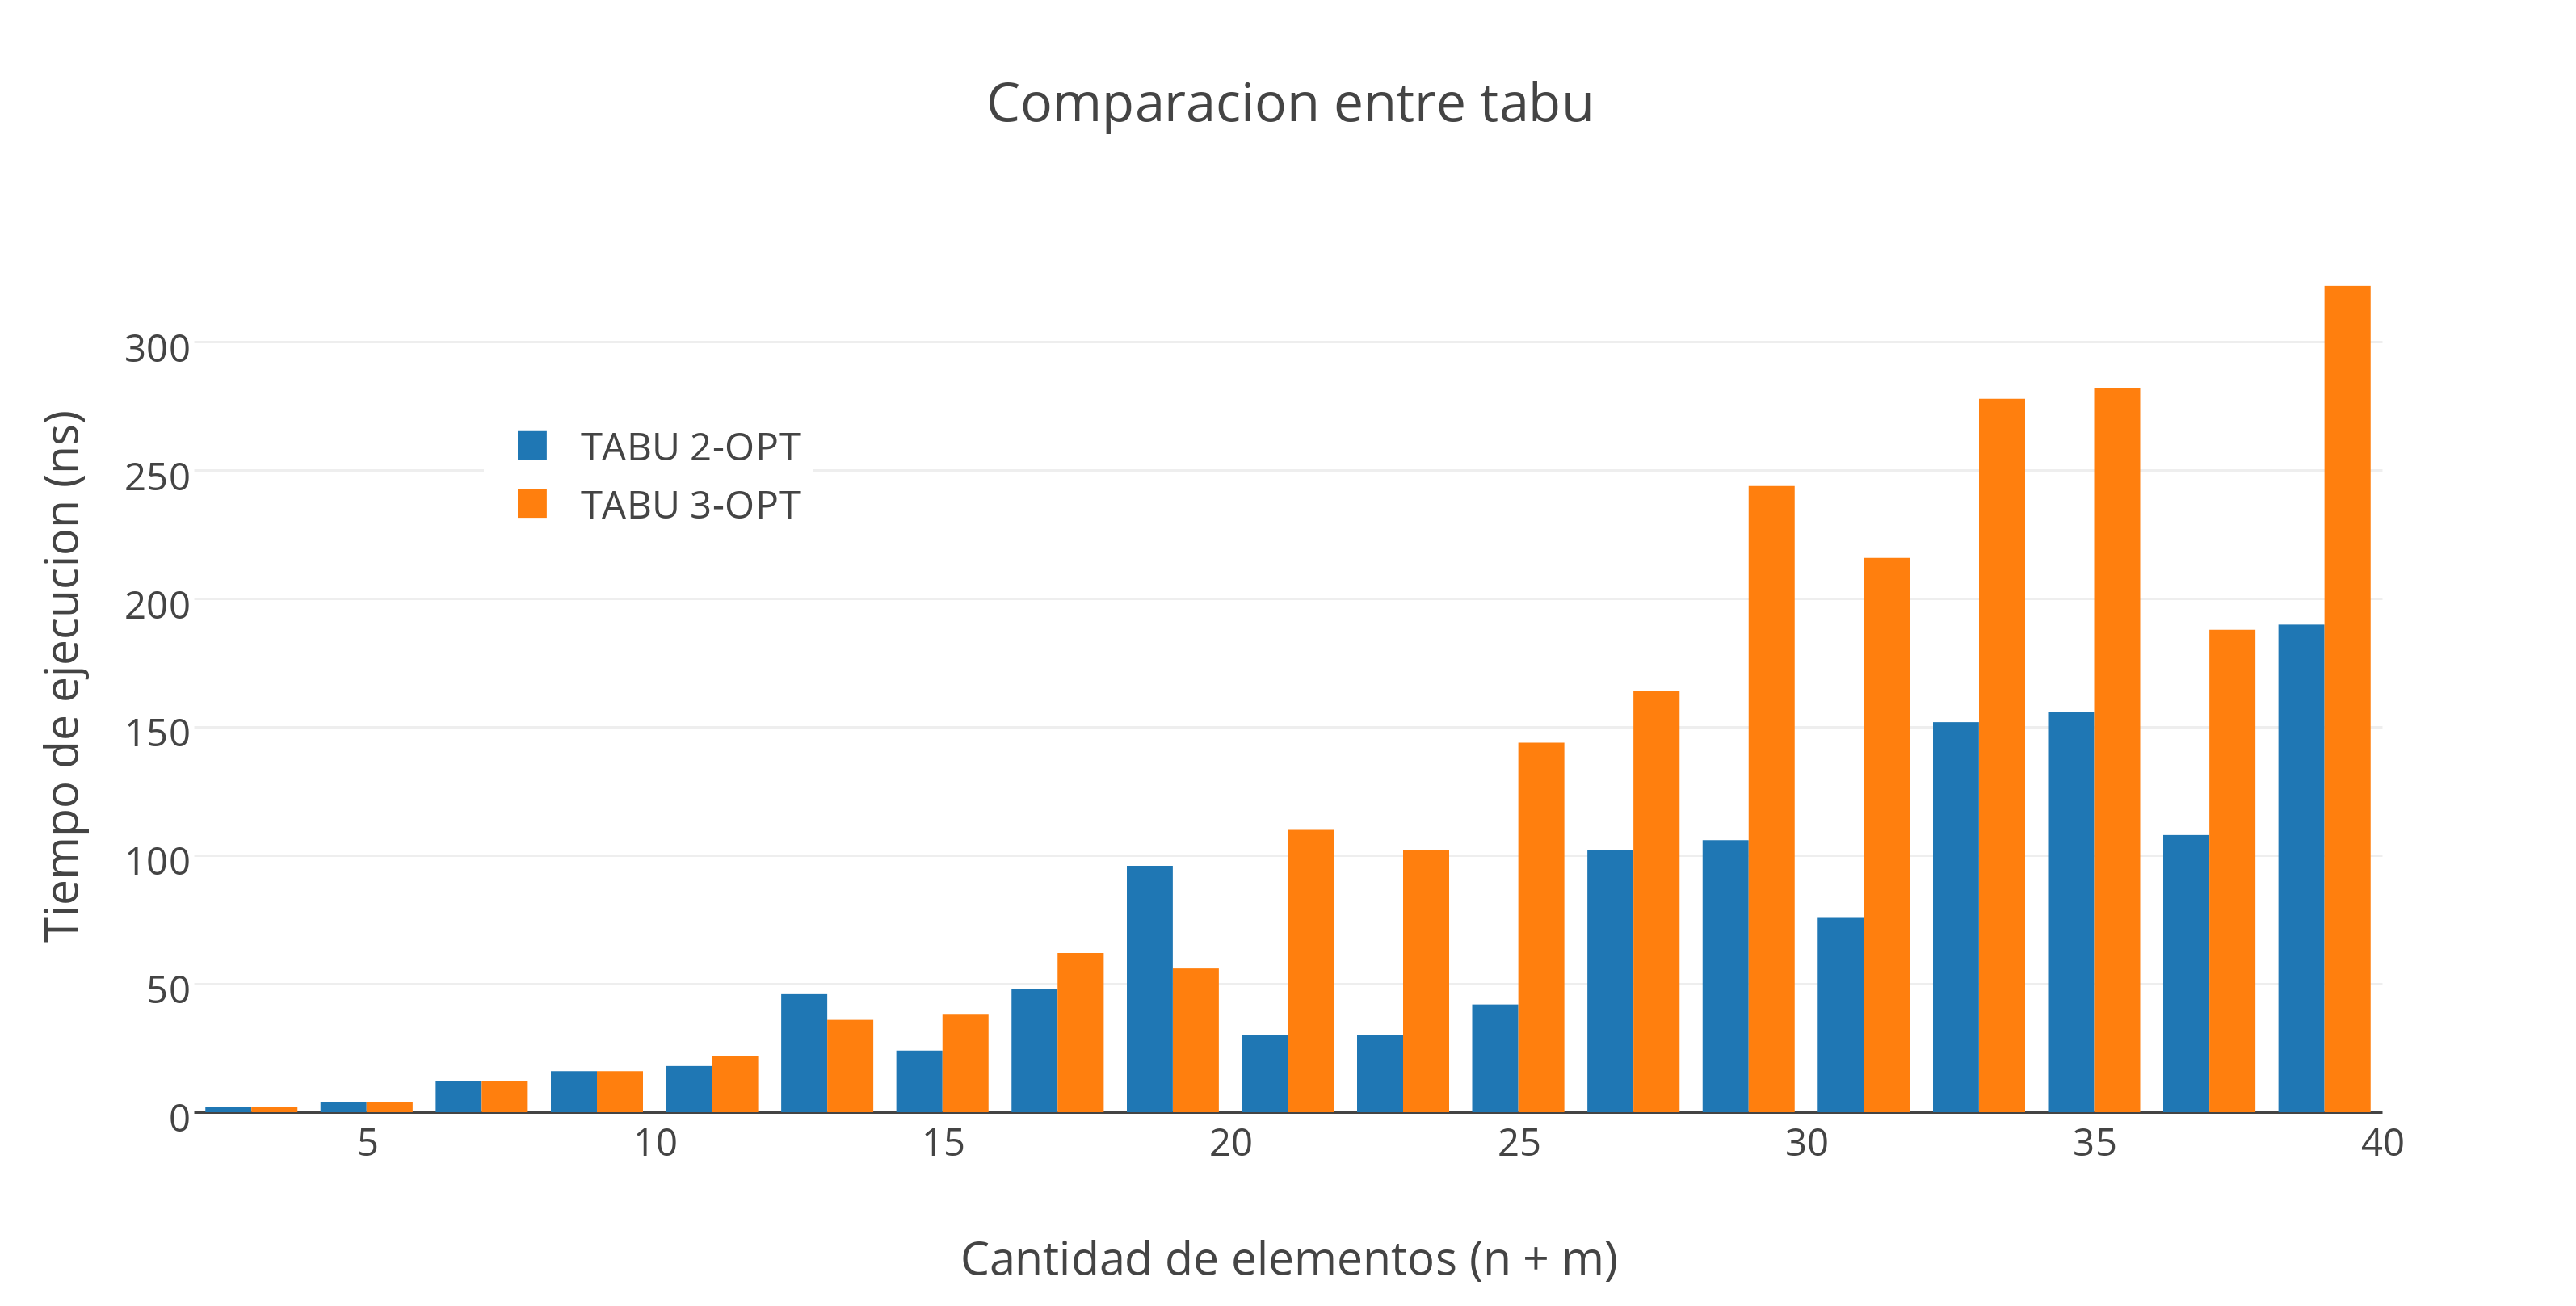
\includegraphics[scale=0.5]{./EJ4/comparativogym0.png}\\
 {            \textit{Gráfico \ 4.5 - Tabu 2-OPT vs Tabu 3-OPT sobre Familia 4}}
  \end{center}
  \vspace*{0.3cm}

En cuanto a tiempo insumido vemos lo siguiente:

\vspace*{0.3cm} \vspace*{0.3cm}
  \begin{center}
 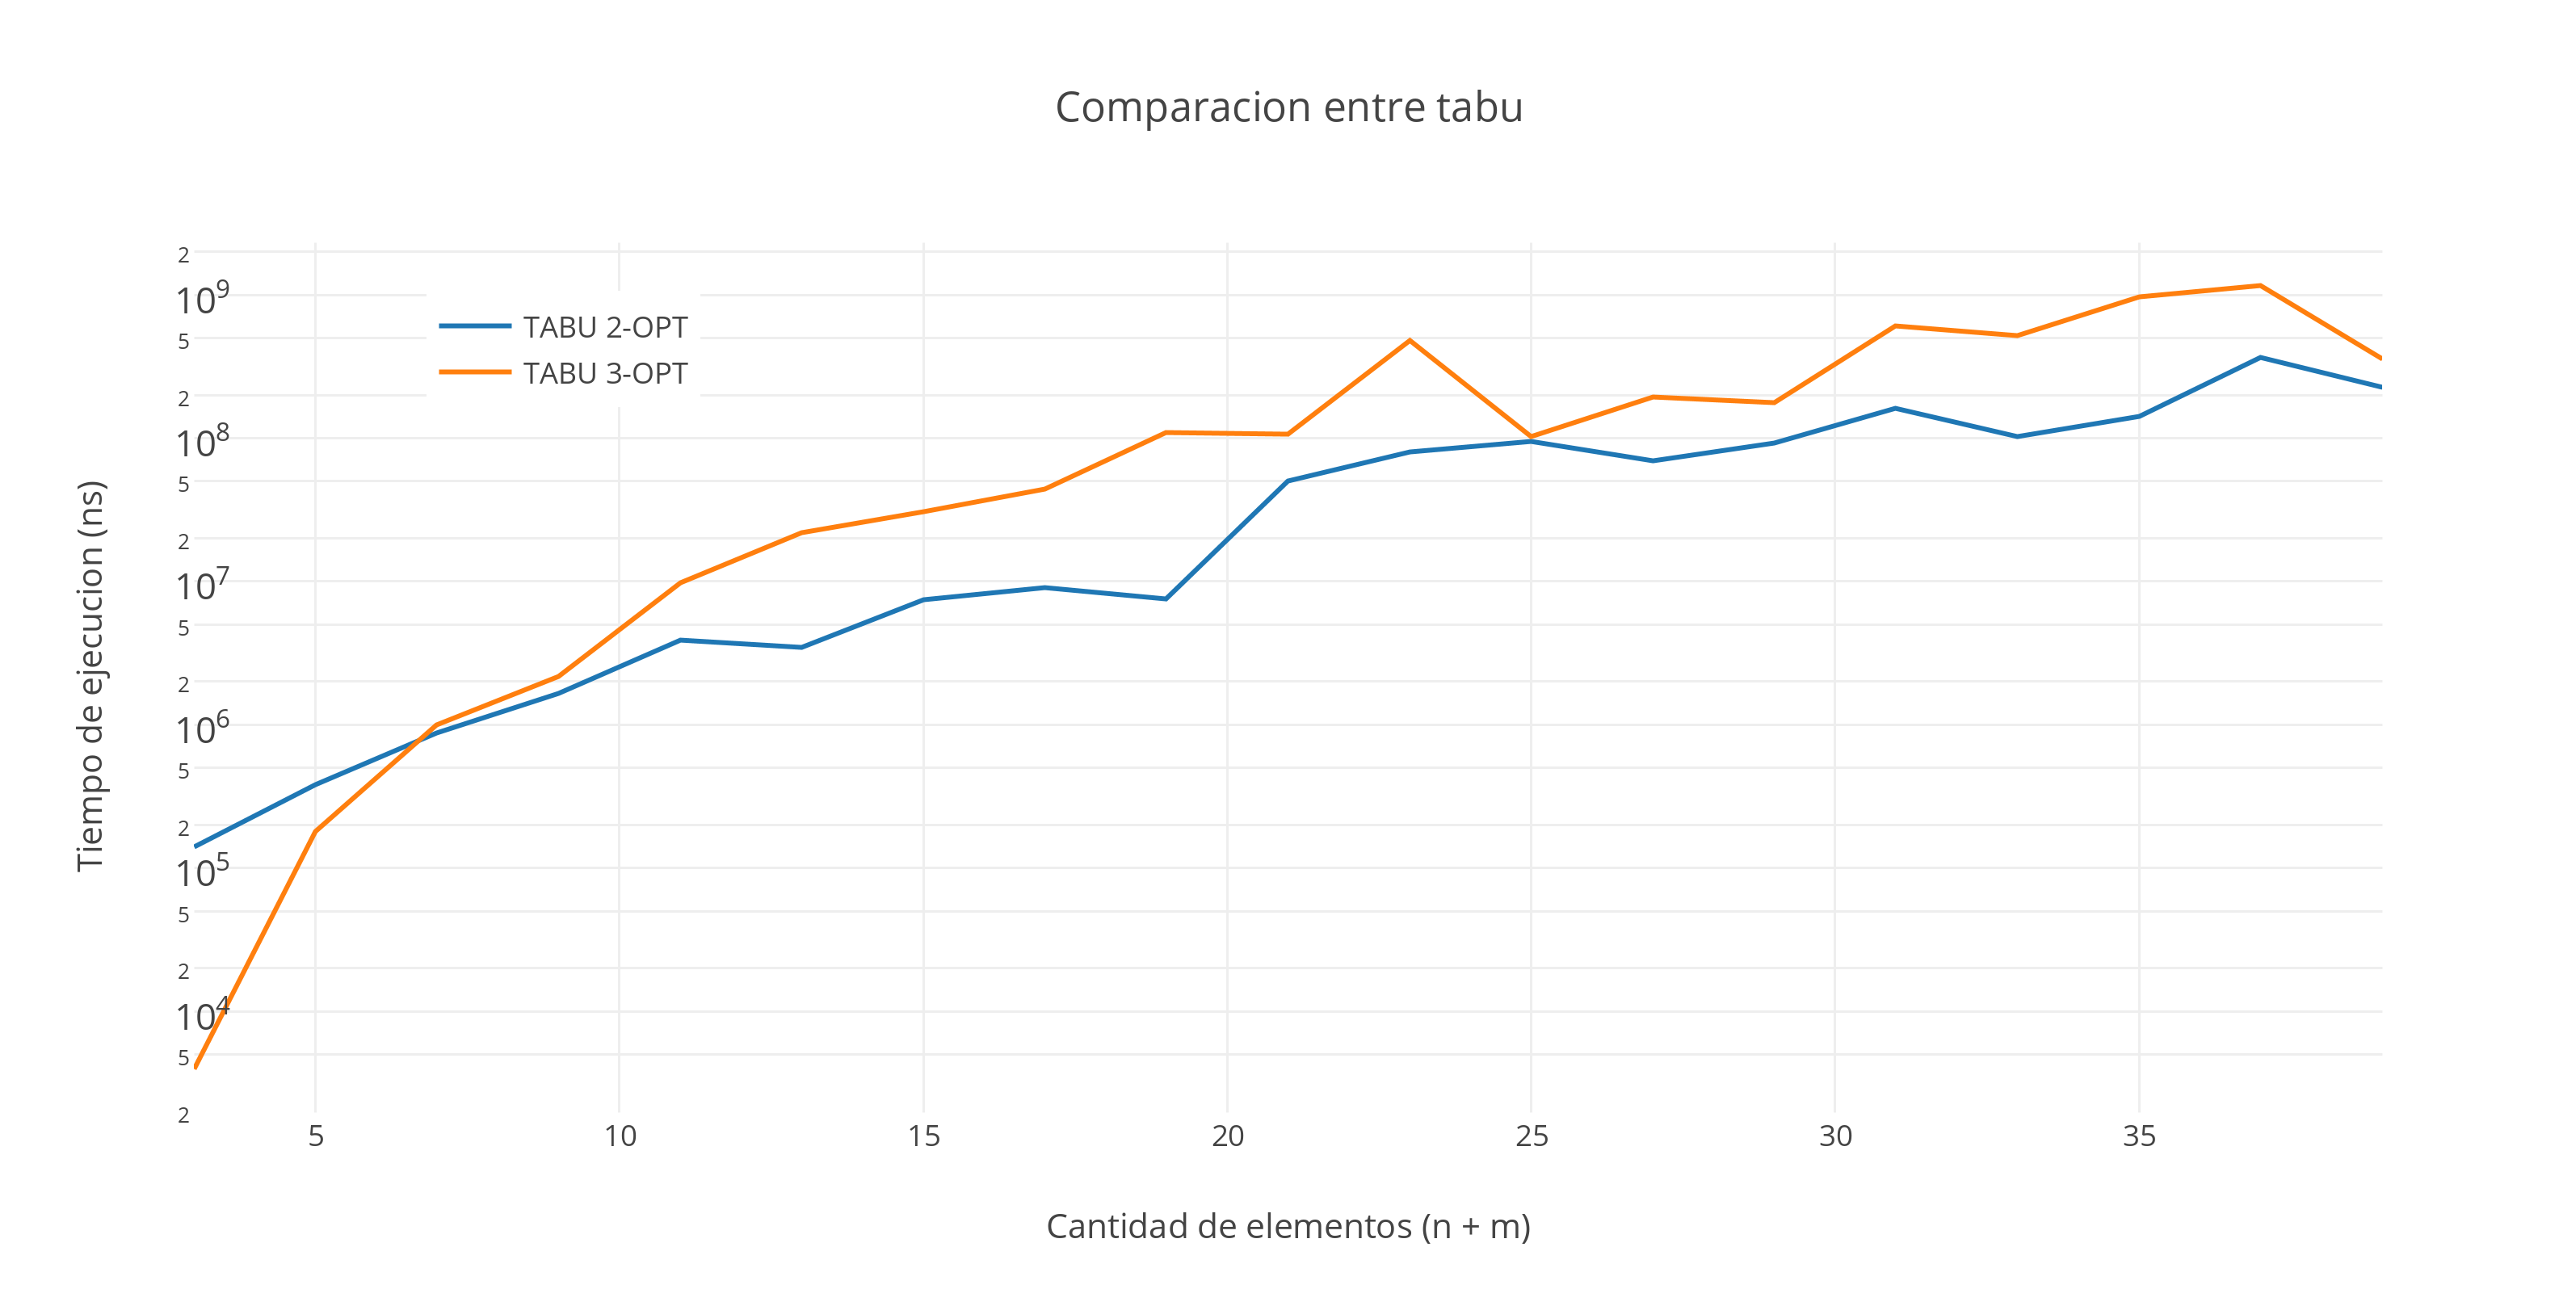
\includegraphics[scale=0.5]{./EJ4/comparaciongym01.png}\\
 {            \textit{Gráfico \ 4.6 - Tabu 2-OPT vs Tabu 3-OPT sobre Familia 4}}
  \end{center}
  \vspace*{0.3cm}

--> OBTENER CONCLUSIONES

\subsubsection*{Familia 6}

--> PRESENTAR FAMILIA

\vspace*{0.3cm} \vspace*{0.3cm}
  \begin{center}
 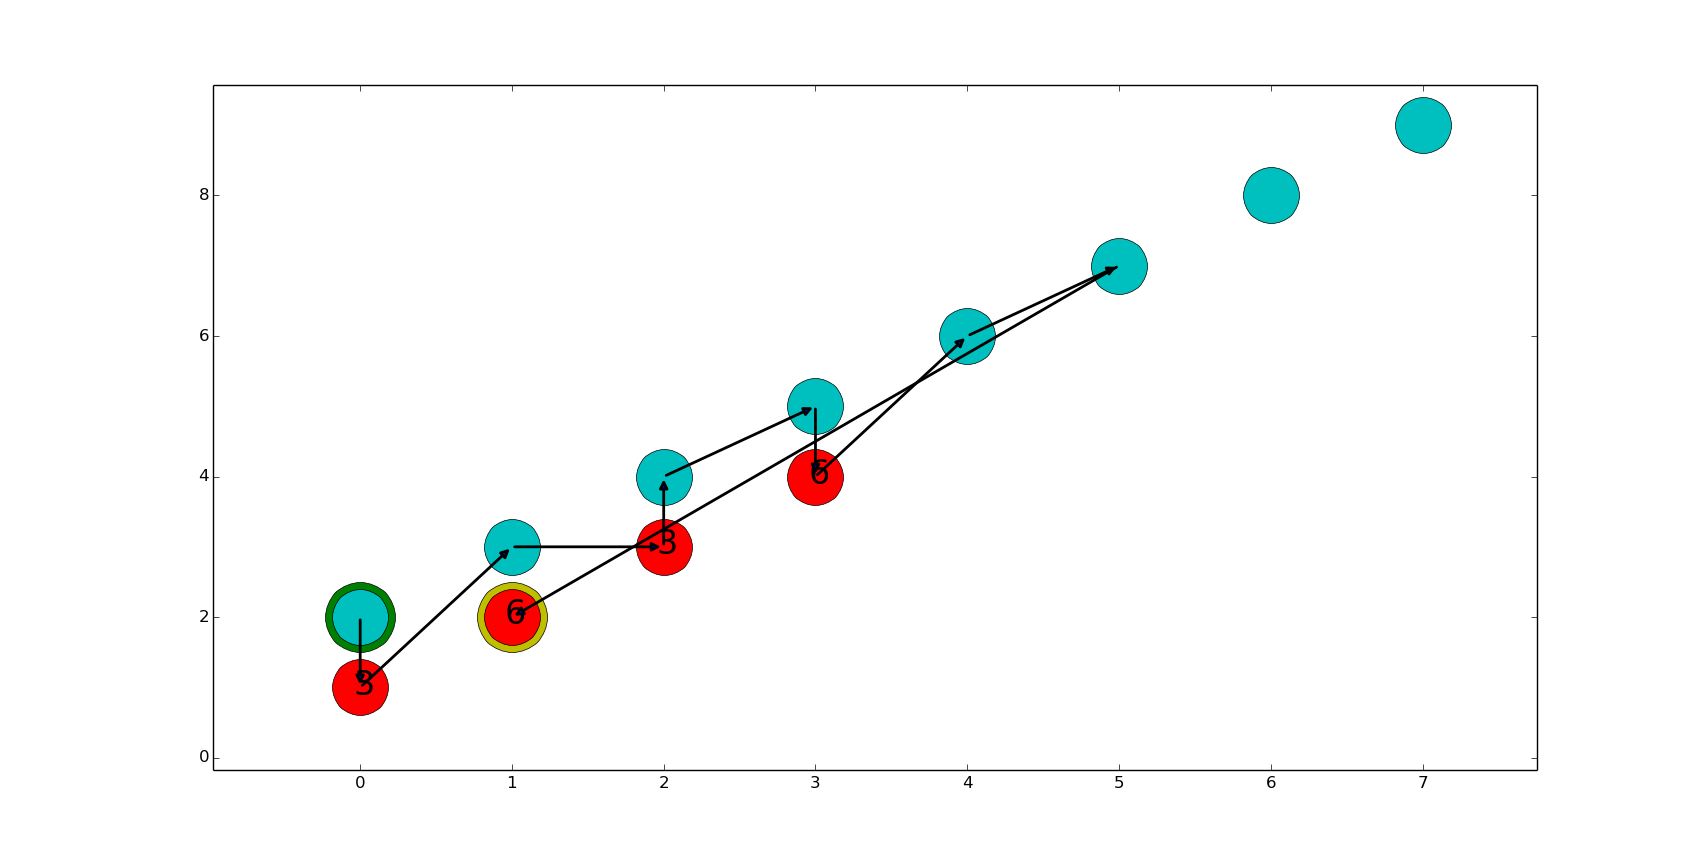
\includegraphics[scale=0.3]{./EJ4/fam6goloso.png}\\
 {            \textit{Soluci\'on Golosa}}
  \end{center}
  \vspace*{0.3cm}

\vspace*{0.3cm} \vspace*{0.3cm}
  \begin{center}
 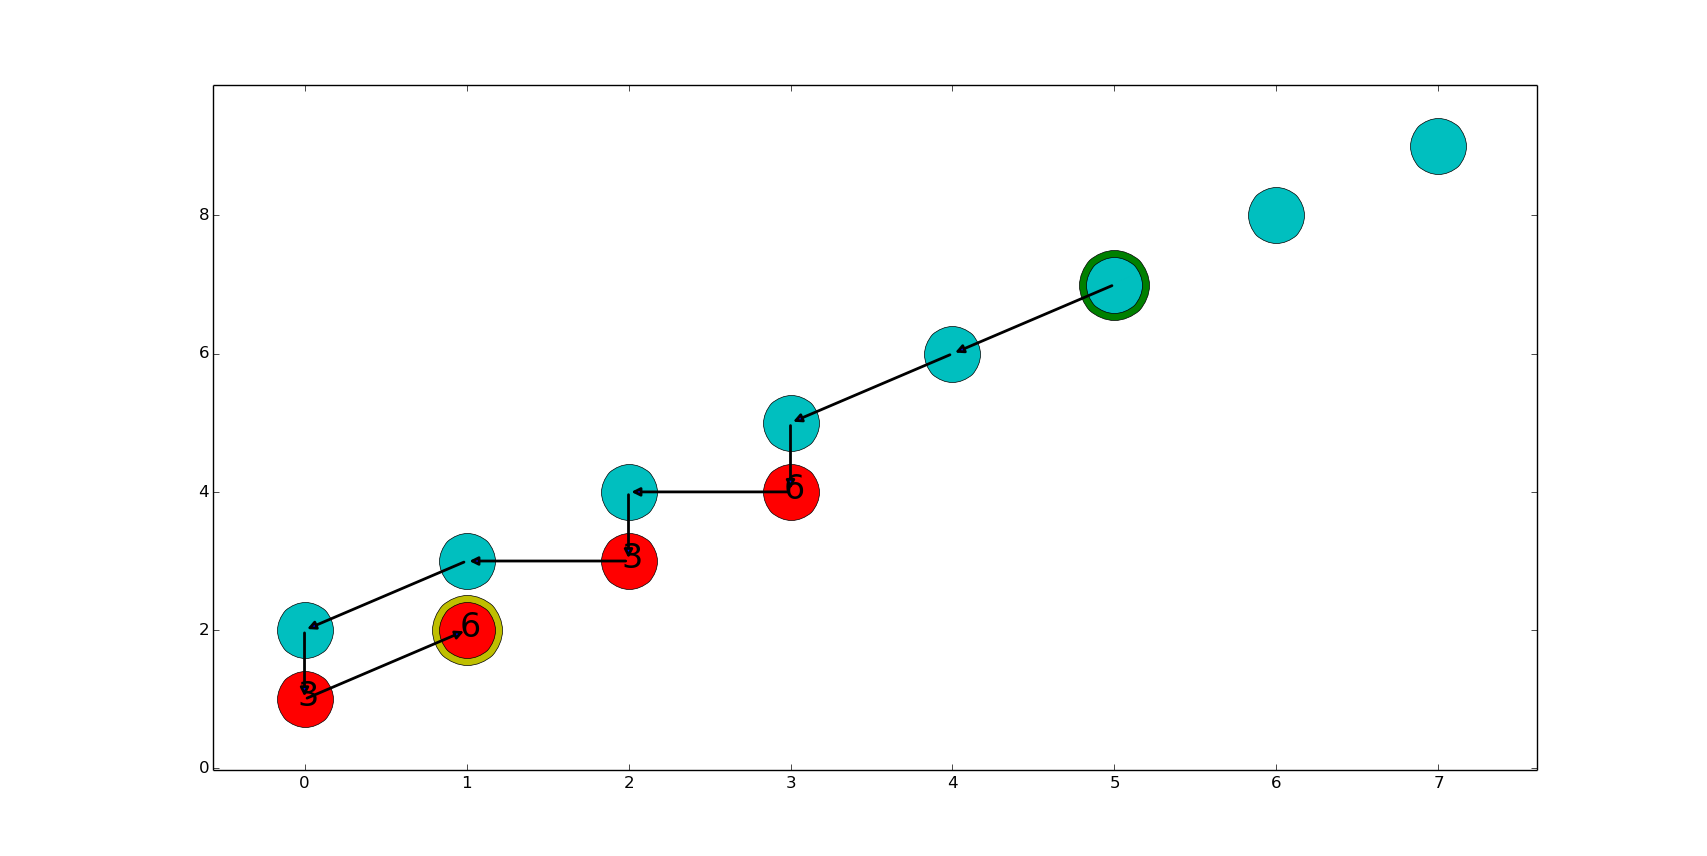
\includegraphics[scale=0.3]{./EJ4/fam62opt.png}\\
 {            \textit{Soluci\'on TABU 2-OPT}}
  \end{center}
  \vspace*{0.3cm}

\vspace*{0.3cm} \vspace*{0.3cm}
  \begin{center}
 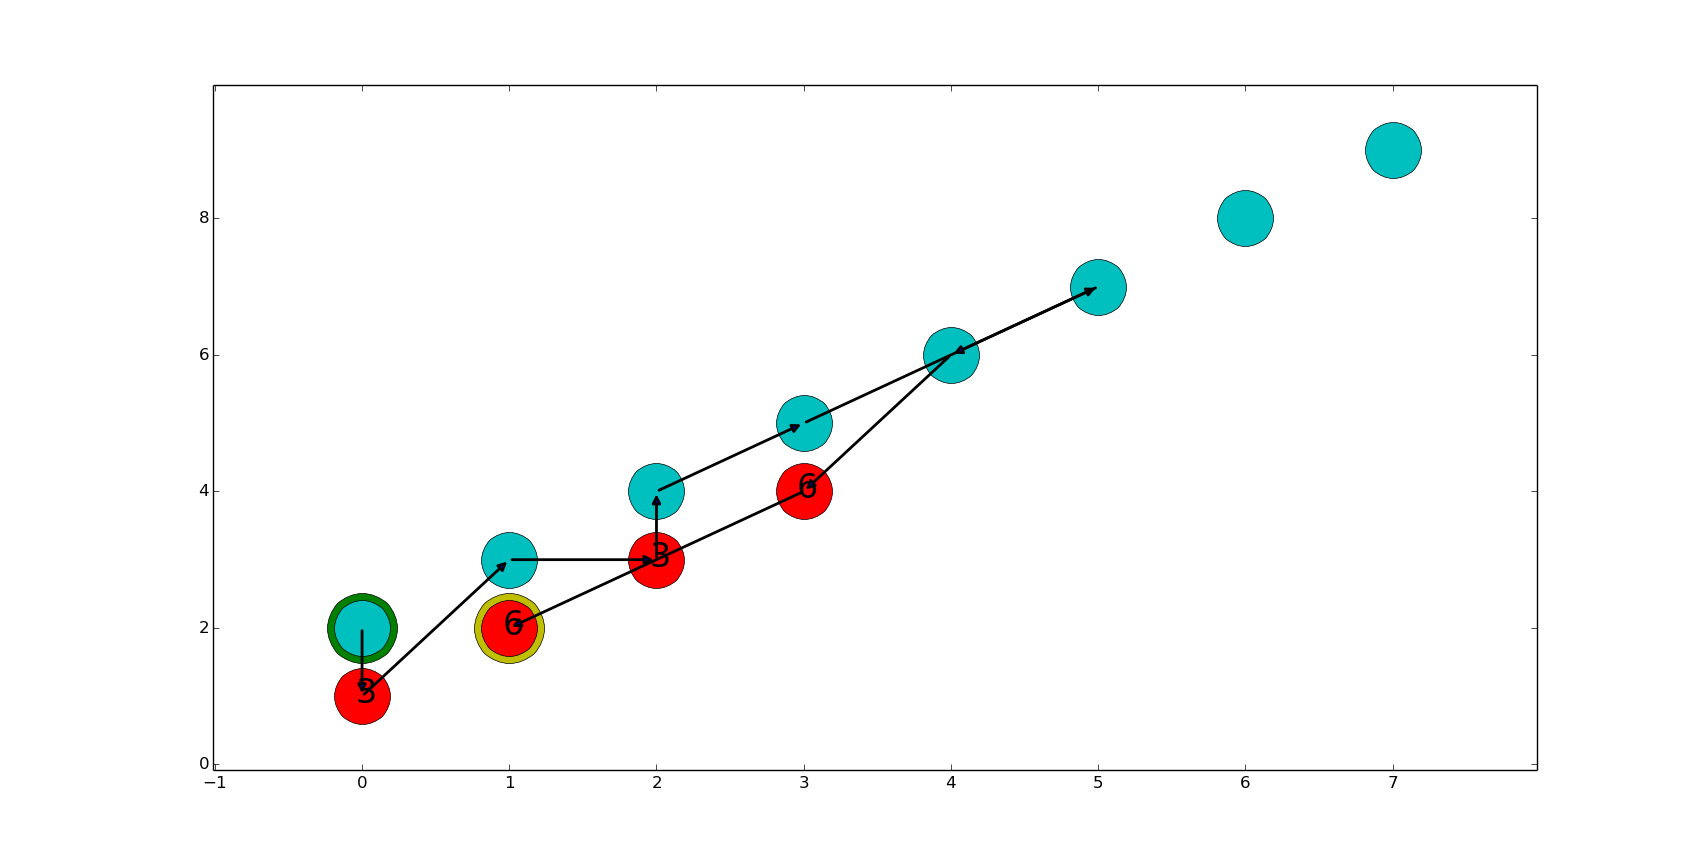
\includegraphics[scale=0.3]{./EJ4/fam63opt.png}\\
 {            \textit{Soluci\'on TABU 3-OPT}}
  \end{center}
  \vspace*{0.3cm}

Veamos como se comporta Tabu 2-OPT con respecto a la heuristica de busqueda local 2-OPT:

\vspace*{0.3cm} \vspace*{0.3cm}
  \begin{center}
 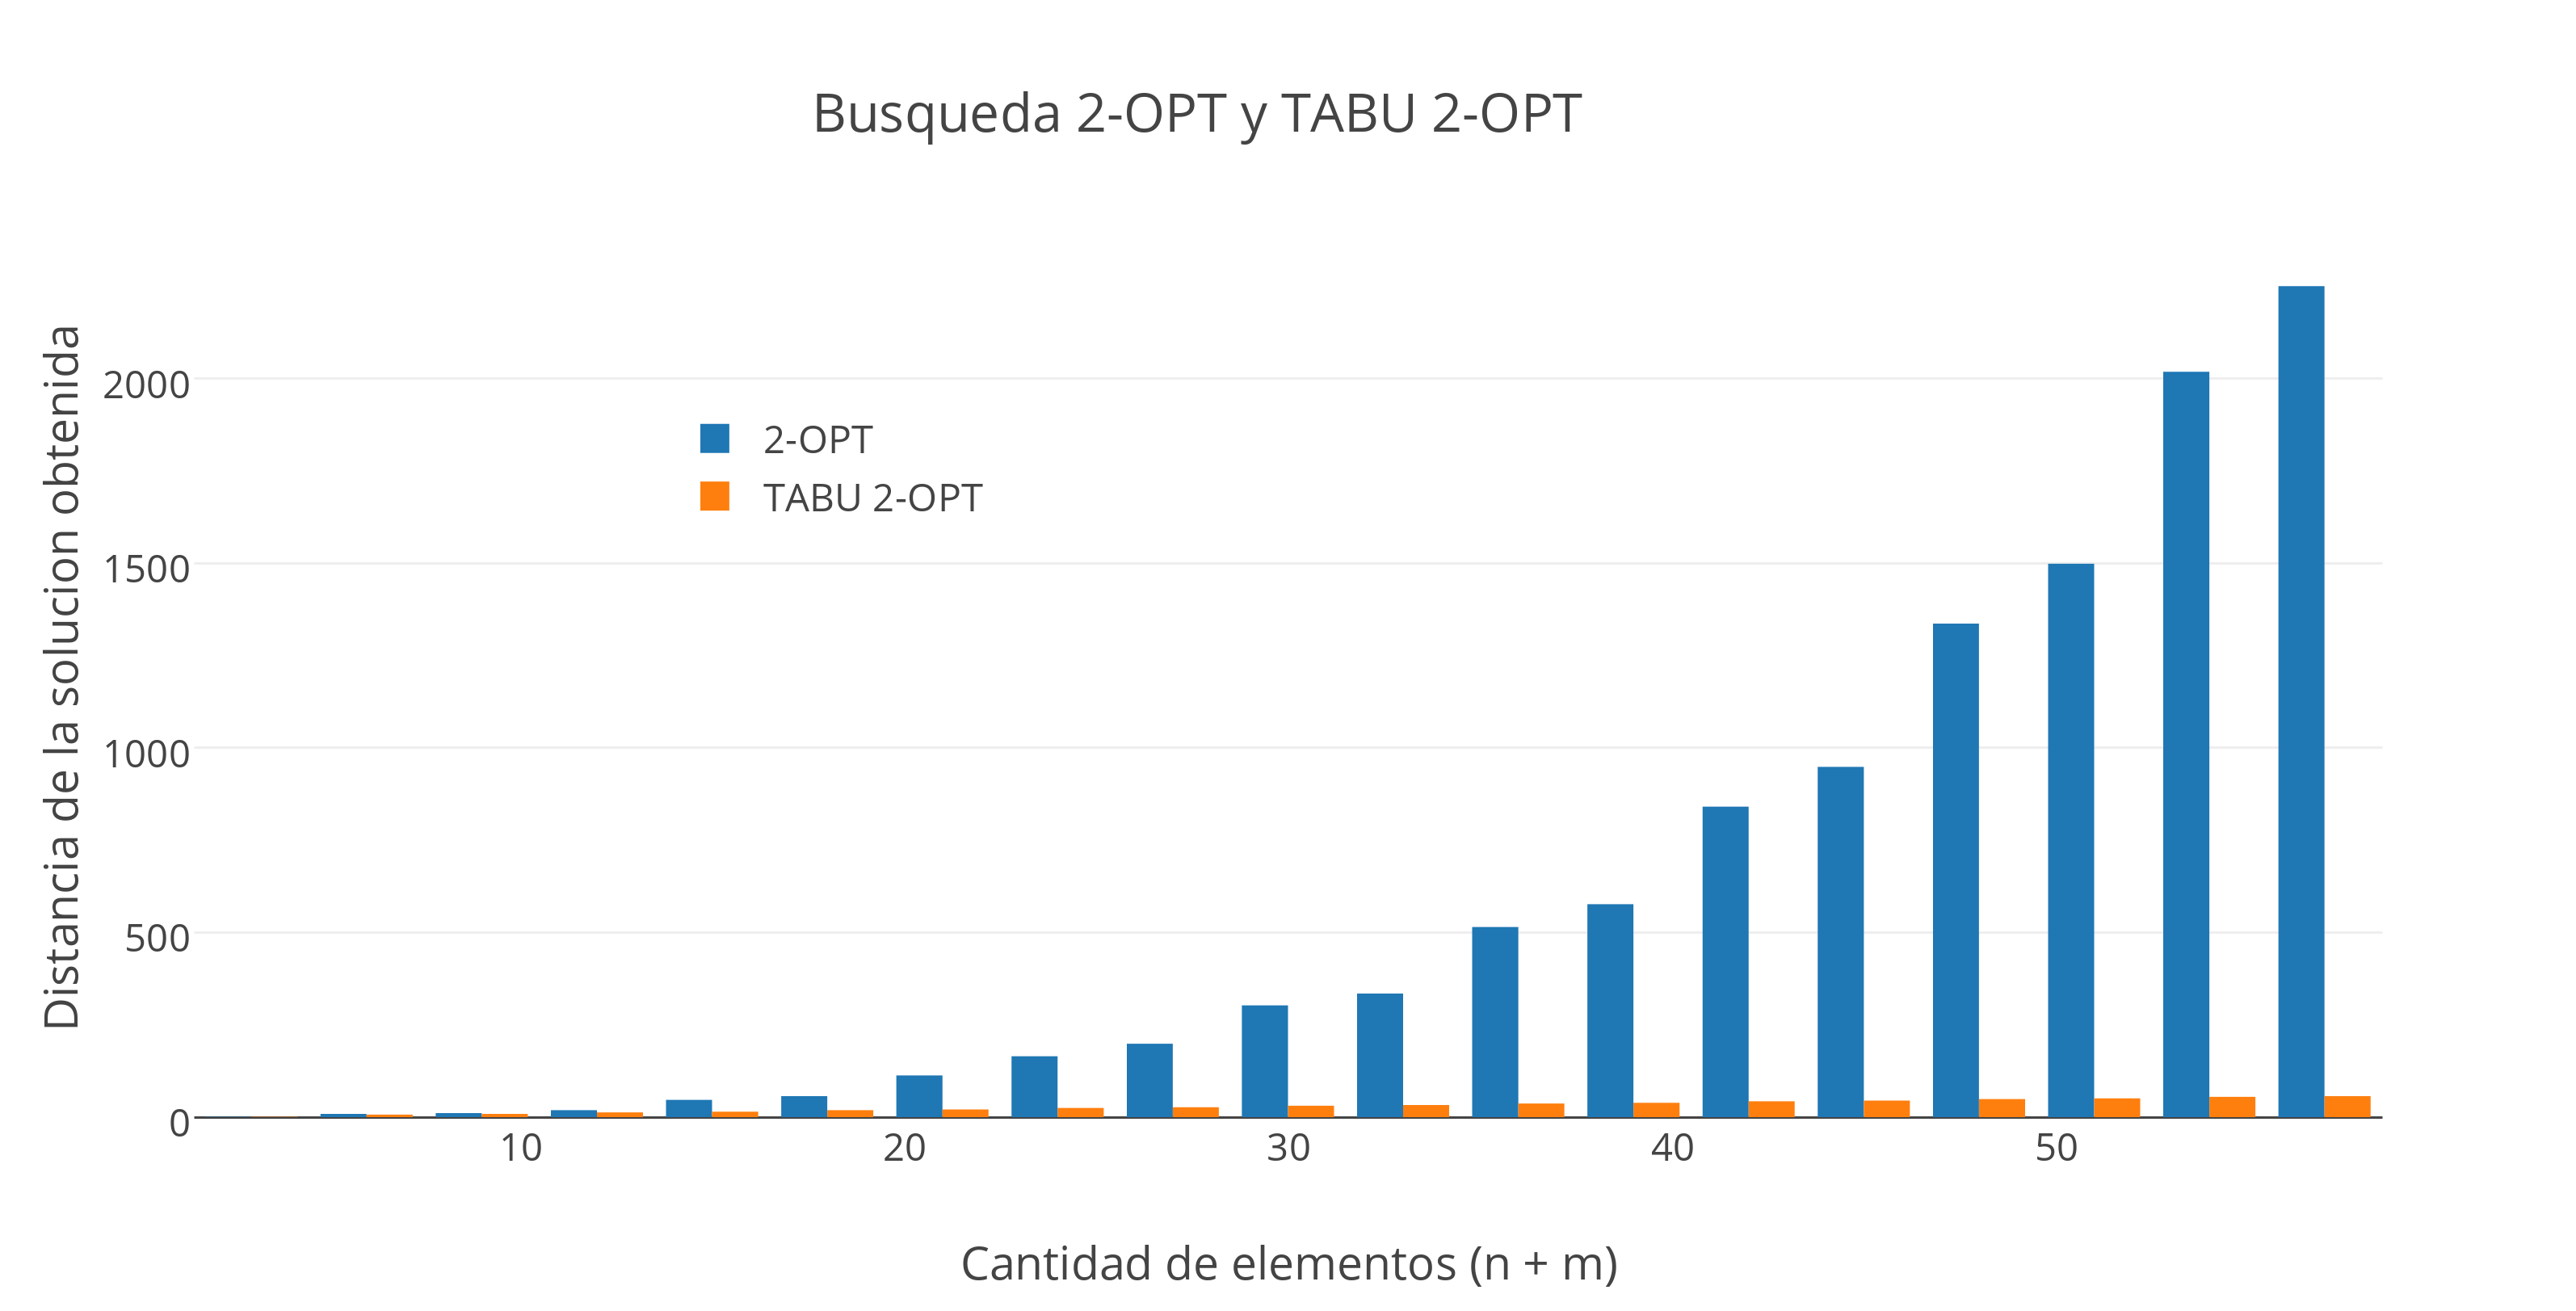
\includegraphics[scale=0.5]{./EJ4/comparativosinorden2opt.png}\\
 {            \textit{Gráfico \ 4.7 - 2-OPT vs Tabu 2-OPT sobre Familia 6}}
  \end{center}
  \vspace*{0.3cm}

\vspace*{0.3cm} \vspace*{0.3cm}
  \begin{center}
 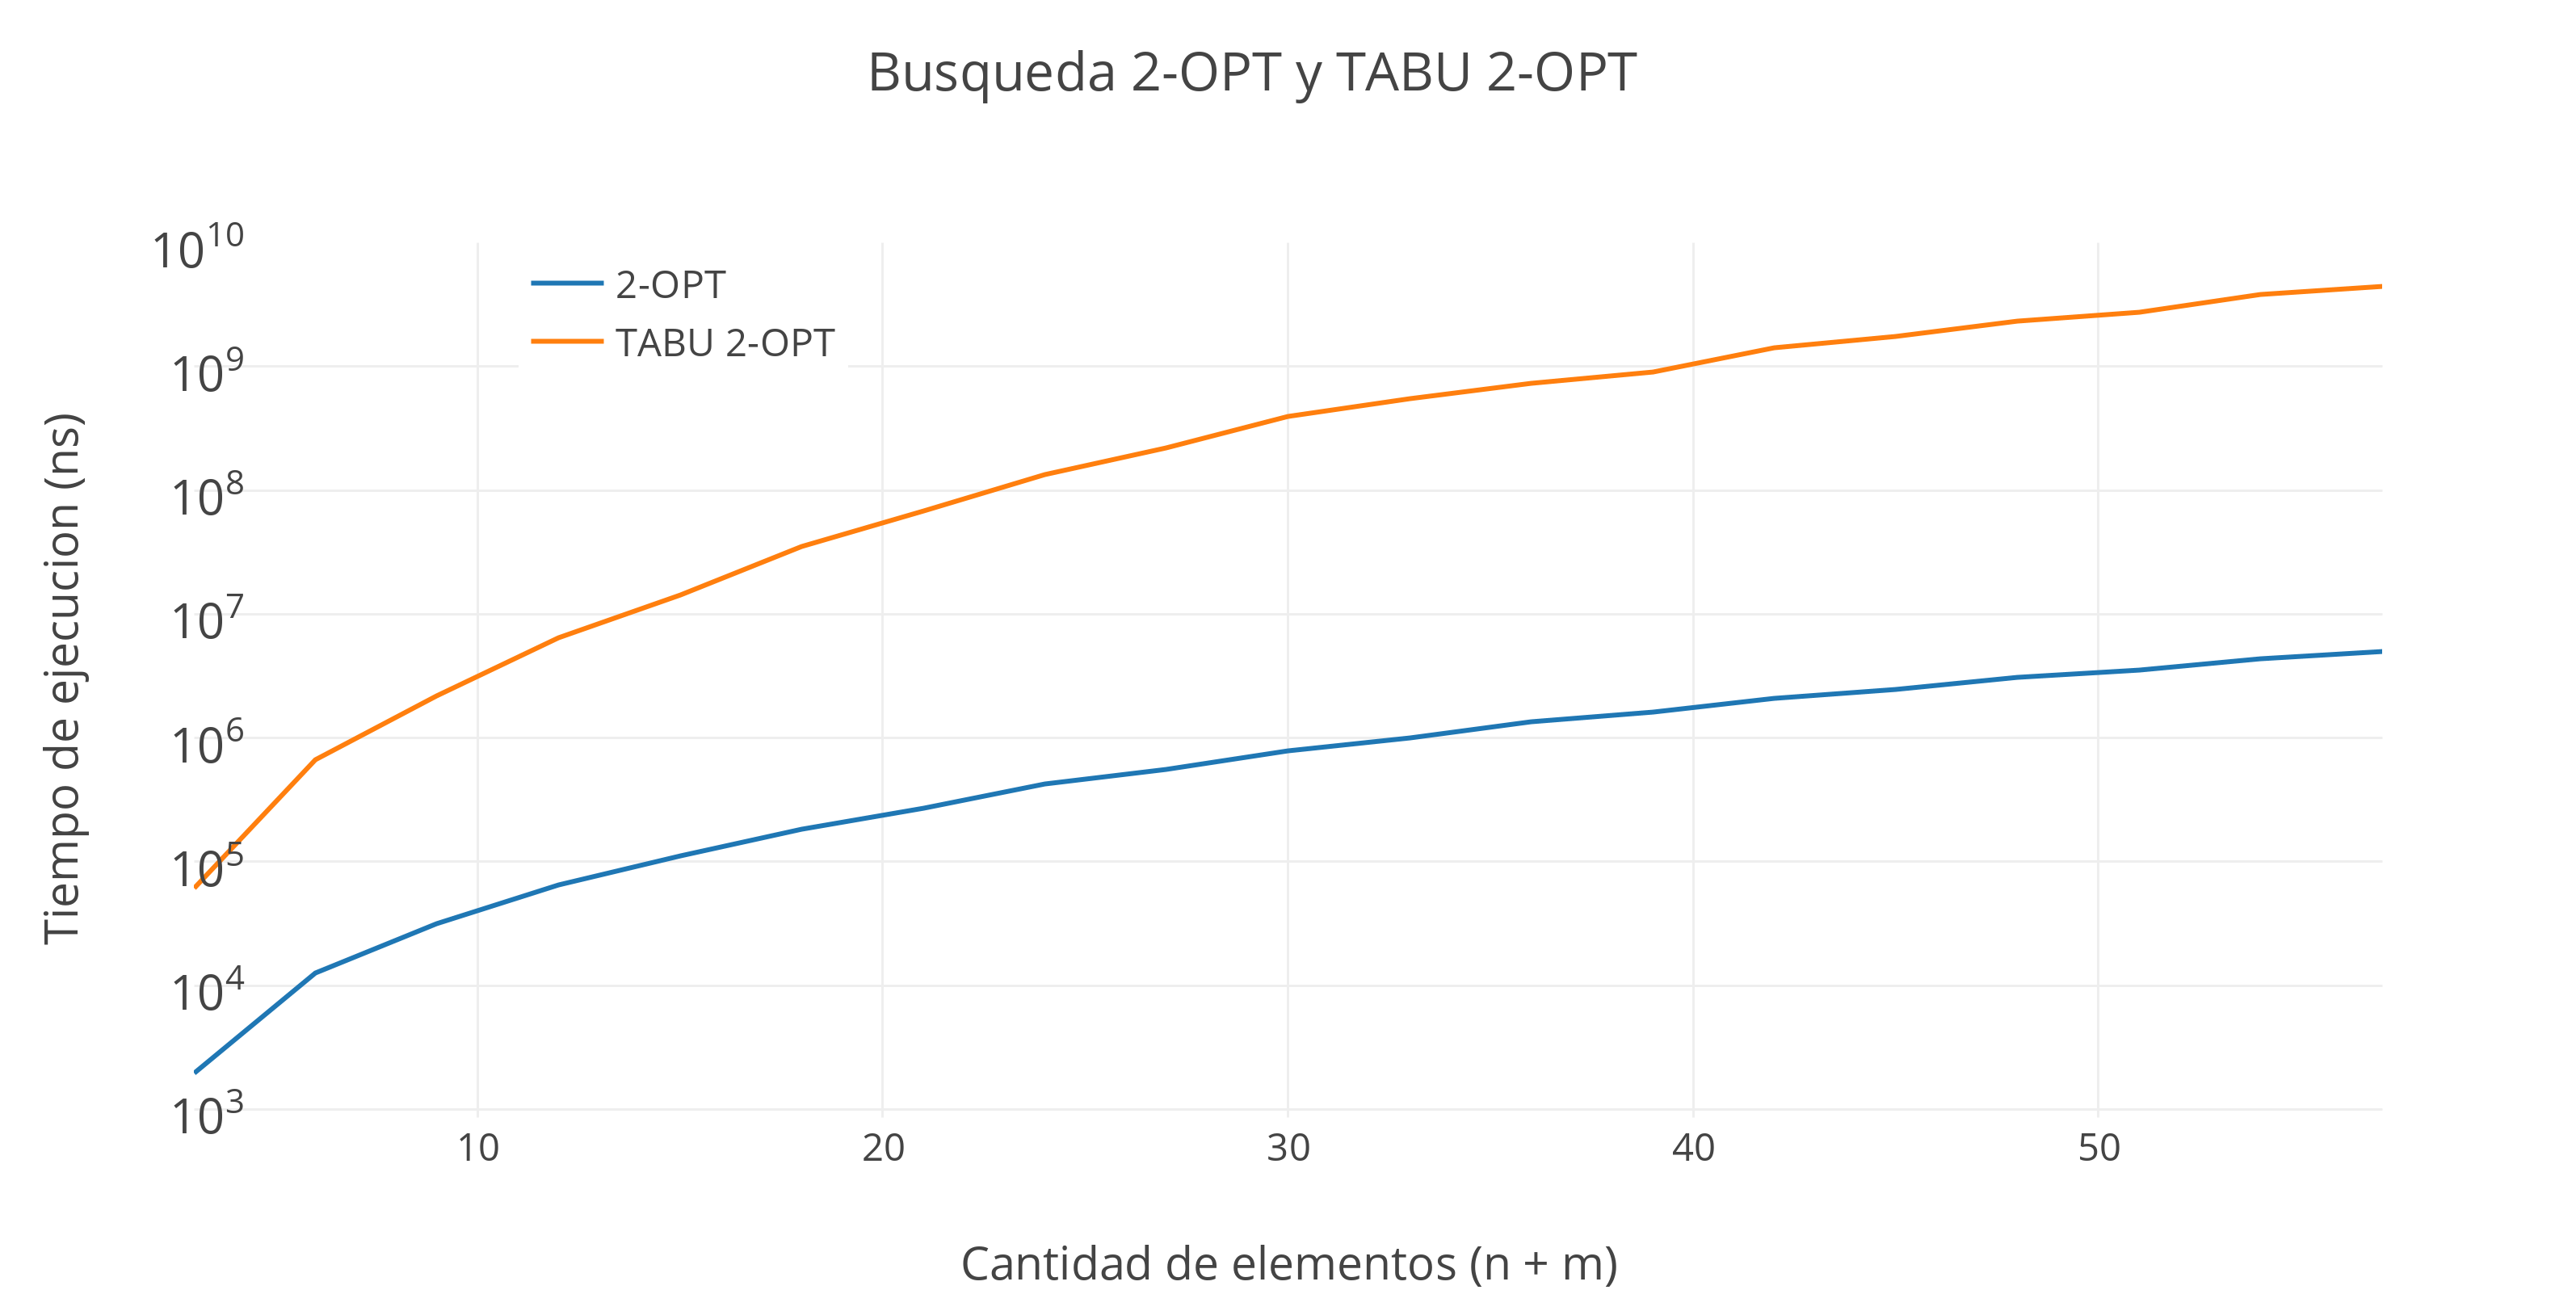
\includegraphics[scale=0.5]{./EJ4/medicion2optsinorden.png}\\
 {            \textit{Gráfico \ 4.8 - 2-OPT vs Tabu 2-OPT sobre Familia 6}}
  \end{center}
  \vspace*{0.3cm}

Luego, para 3-OPT:

\vspace*{0.3cm} \vspace*{0.3cm}
  \begin{center}
 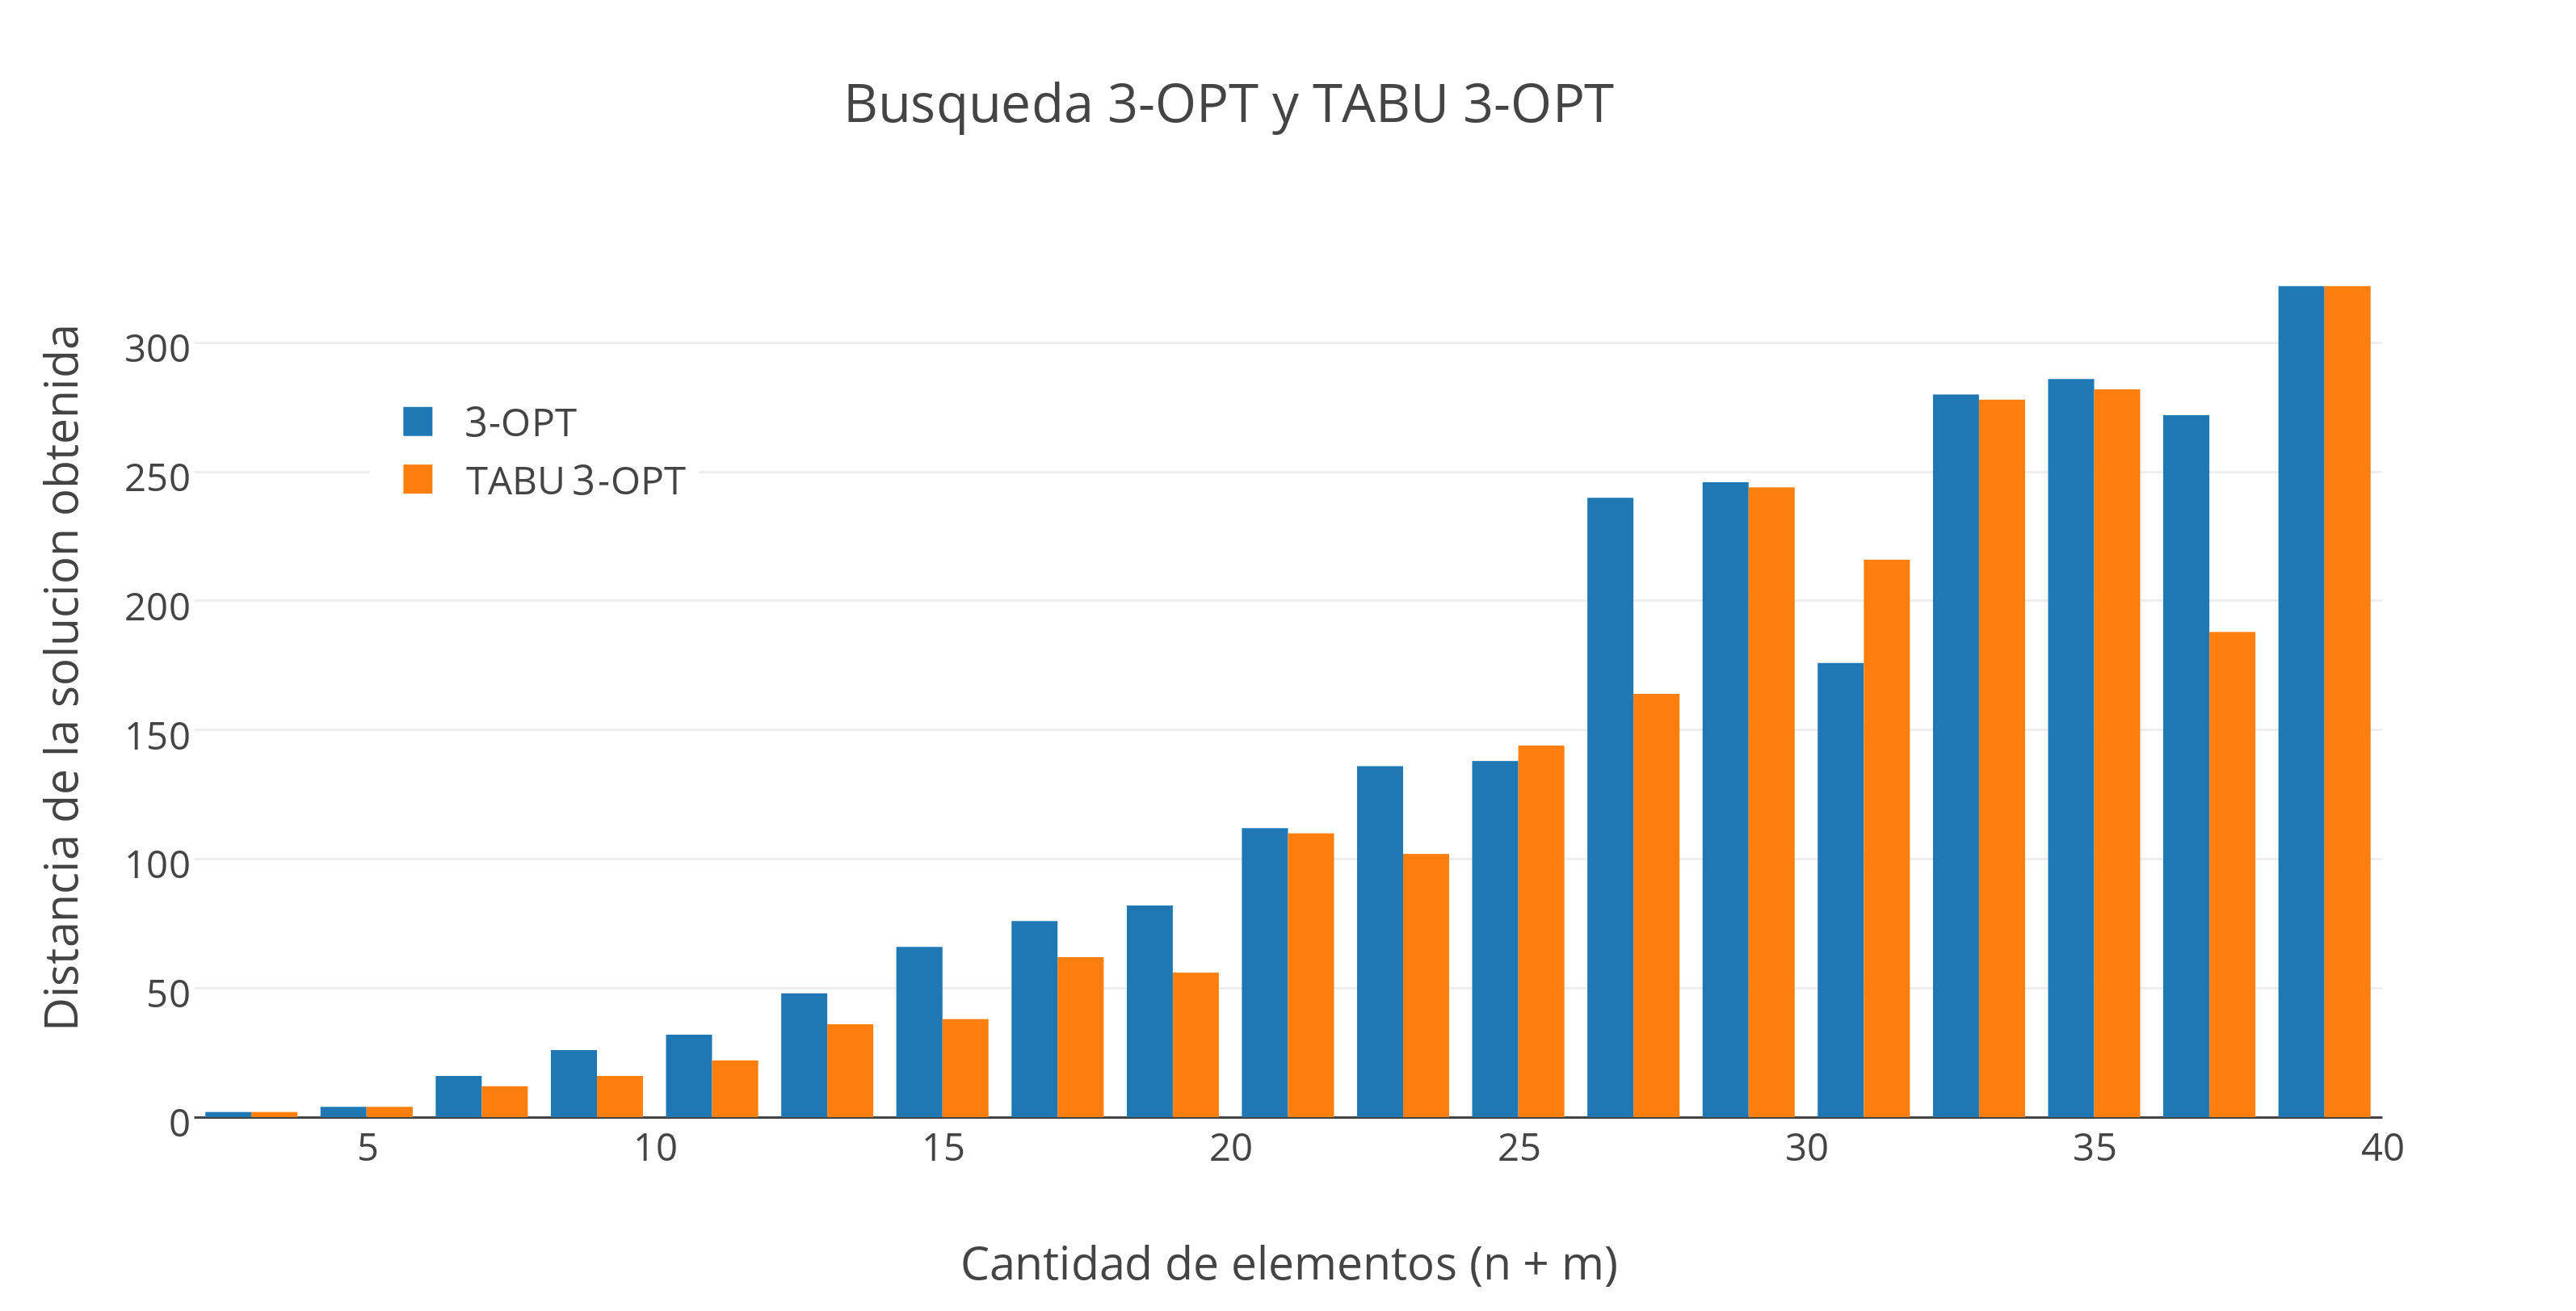
\includegraphics[scale=0.5]{./EJ4/comparativogym03opt.png}\\
 {            \textit{Gráfico \ 4.9 - 3-OPT vs Tabu 3-OPT sobre Familia 6}}
  \end{center}
  \vspace*{0.3cm}

\vspace*{0.3cm} \vspace*{0.3cm}
  \begin{center}
 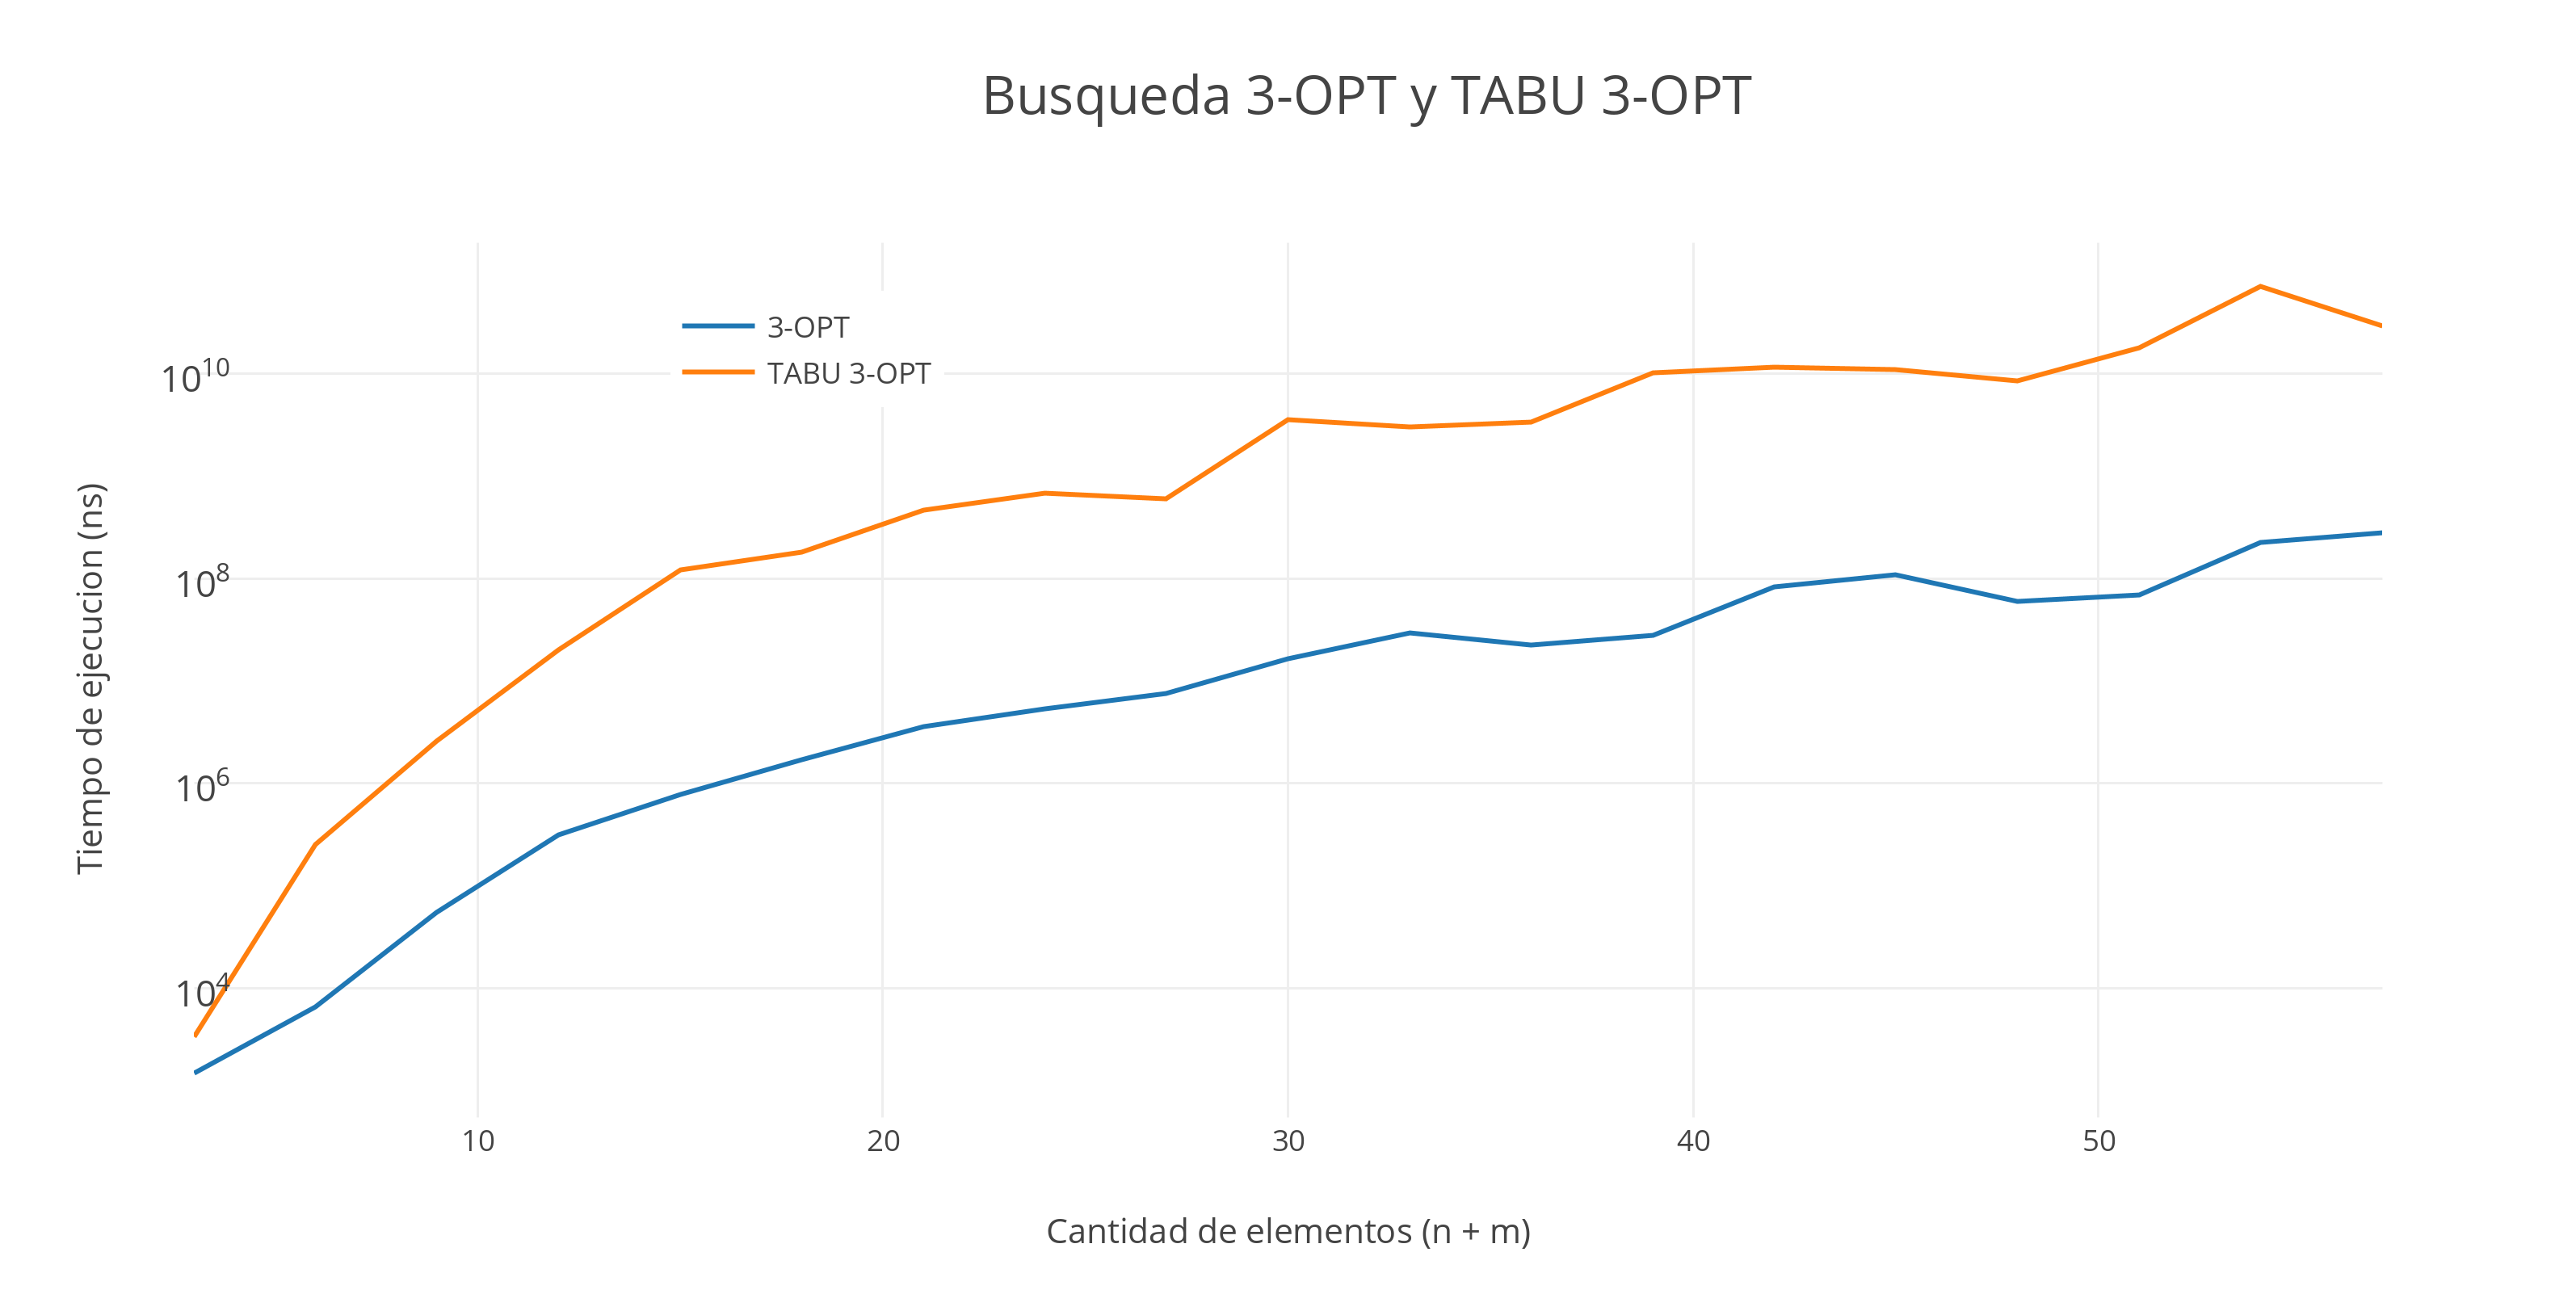
\includegraphics[scale=0.5]{./EJ4/medicion3optsinorden.png}\\
 {            \textit{Gráfico \ 4.10 - 3-OPT vs Tabu 3-OPT sobre Familia 6}}
  \end{center}
  \vspace*{0.3cm}
  
--> OBTENER CONCLUSIONES
  
Comparando las soluciones de cada version de tabú search podemos observar lo siguiente:

\vspace*{0.3cm} \vspace*{0.3cm}
  \begin{center}
 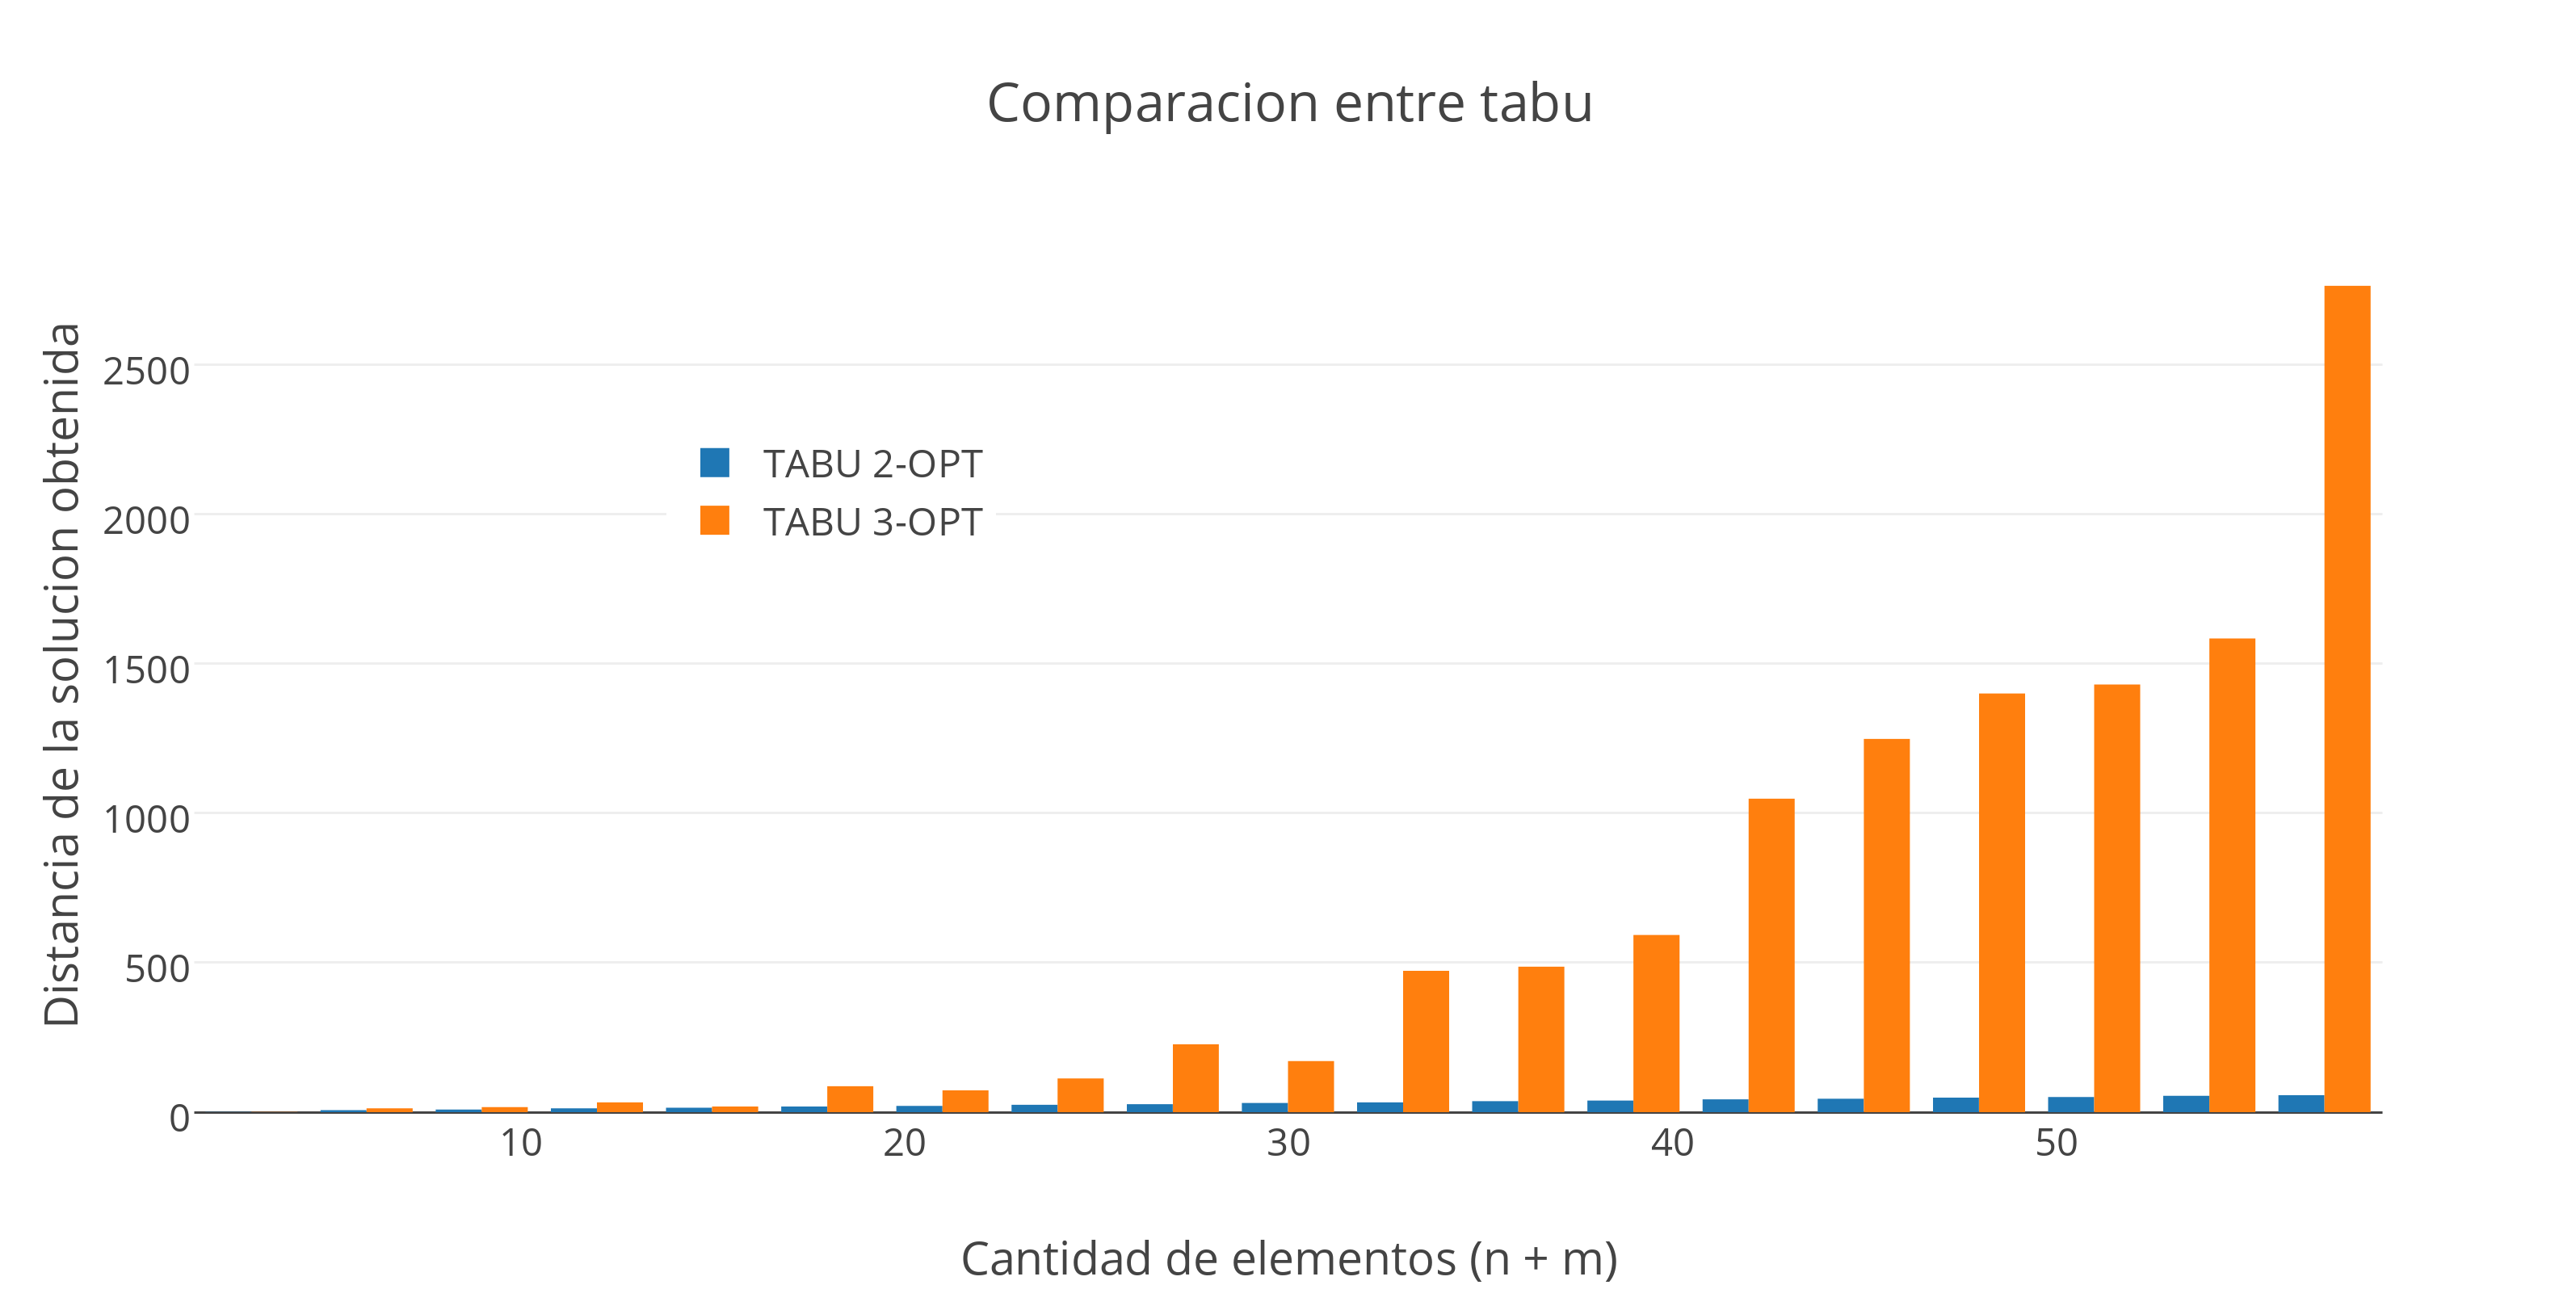
\includegraphics[scale=0.5]{./EJ4/comparativosinorden.png}\\
 {            \textit{Gráfico \ 4.11 - Tabu 2-OPT vs Tabu 3-OPT sobre Familia 6}}
  \end{center}
  \vspace*{0.3cm}

En cuanto a tiempo insumido vemos lo siguiente:

\vspace*{0.3cm} \vspace*{0.3cm}
  \begin{center}
 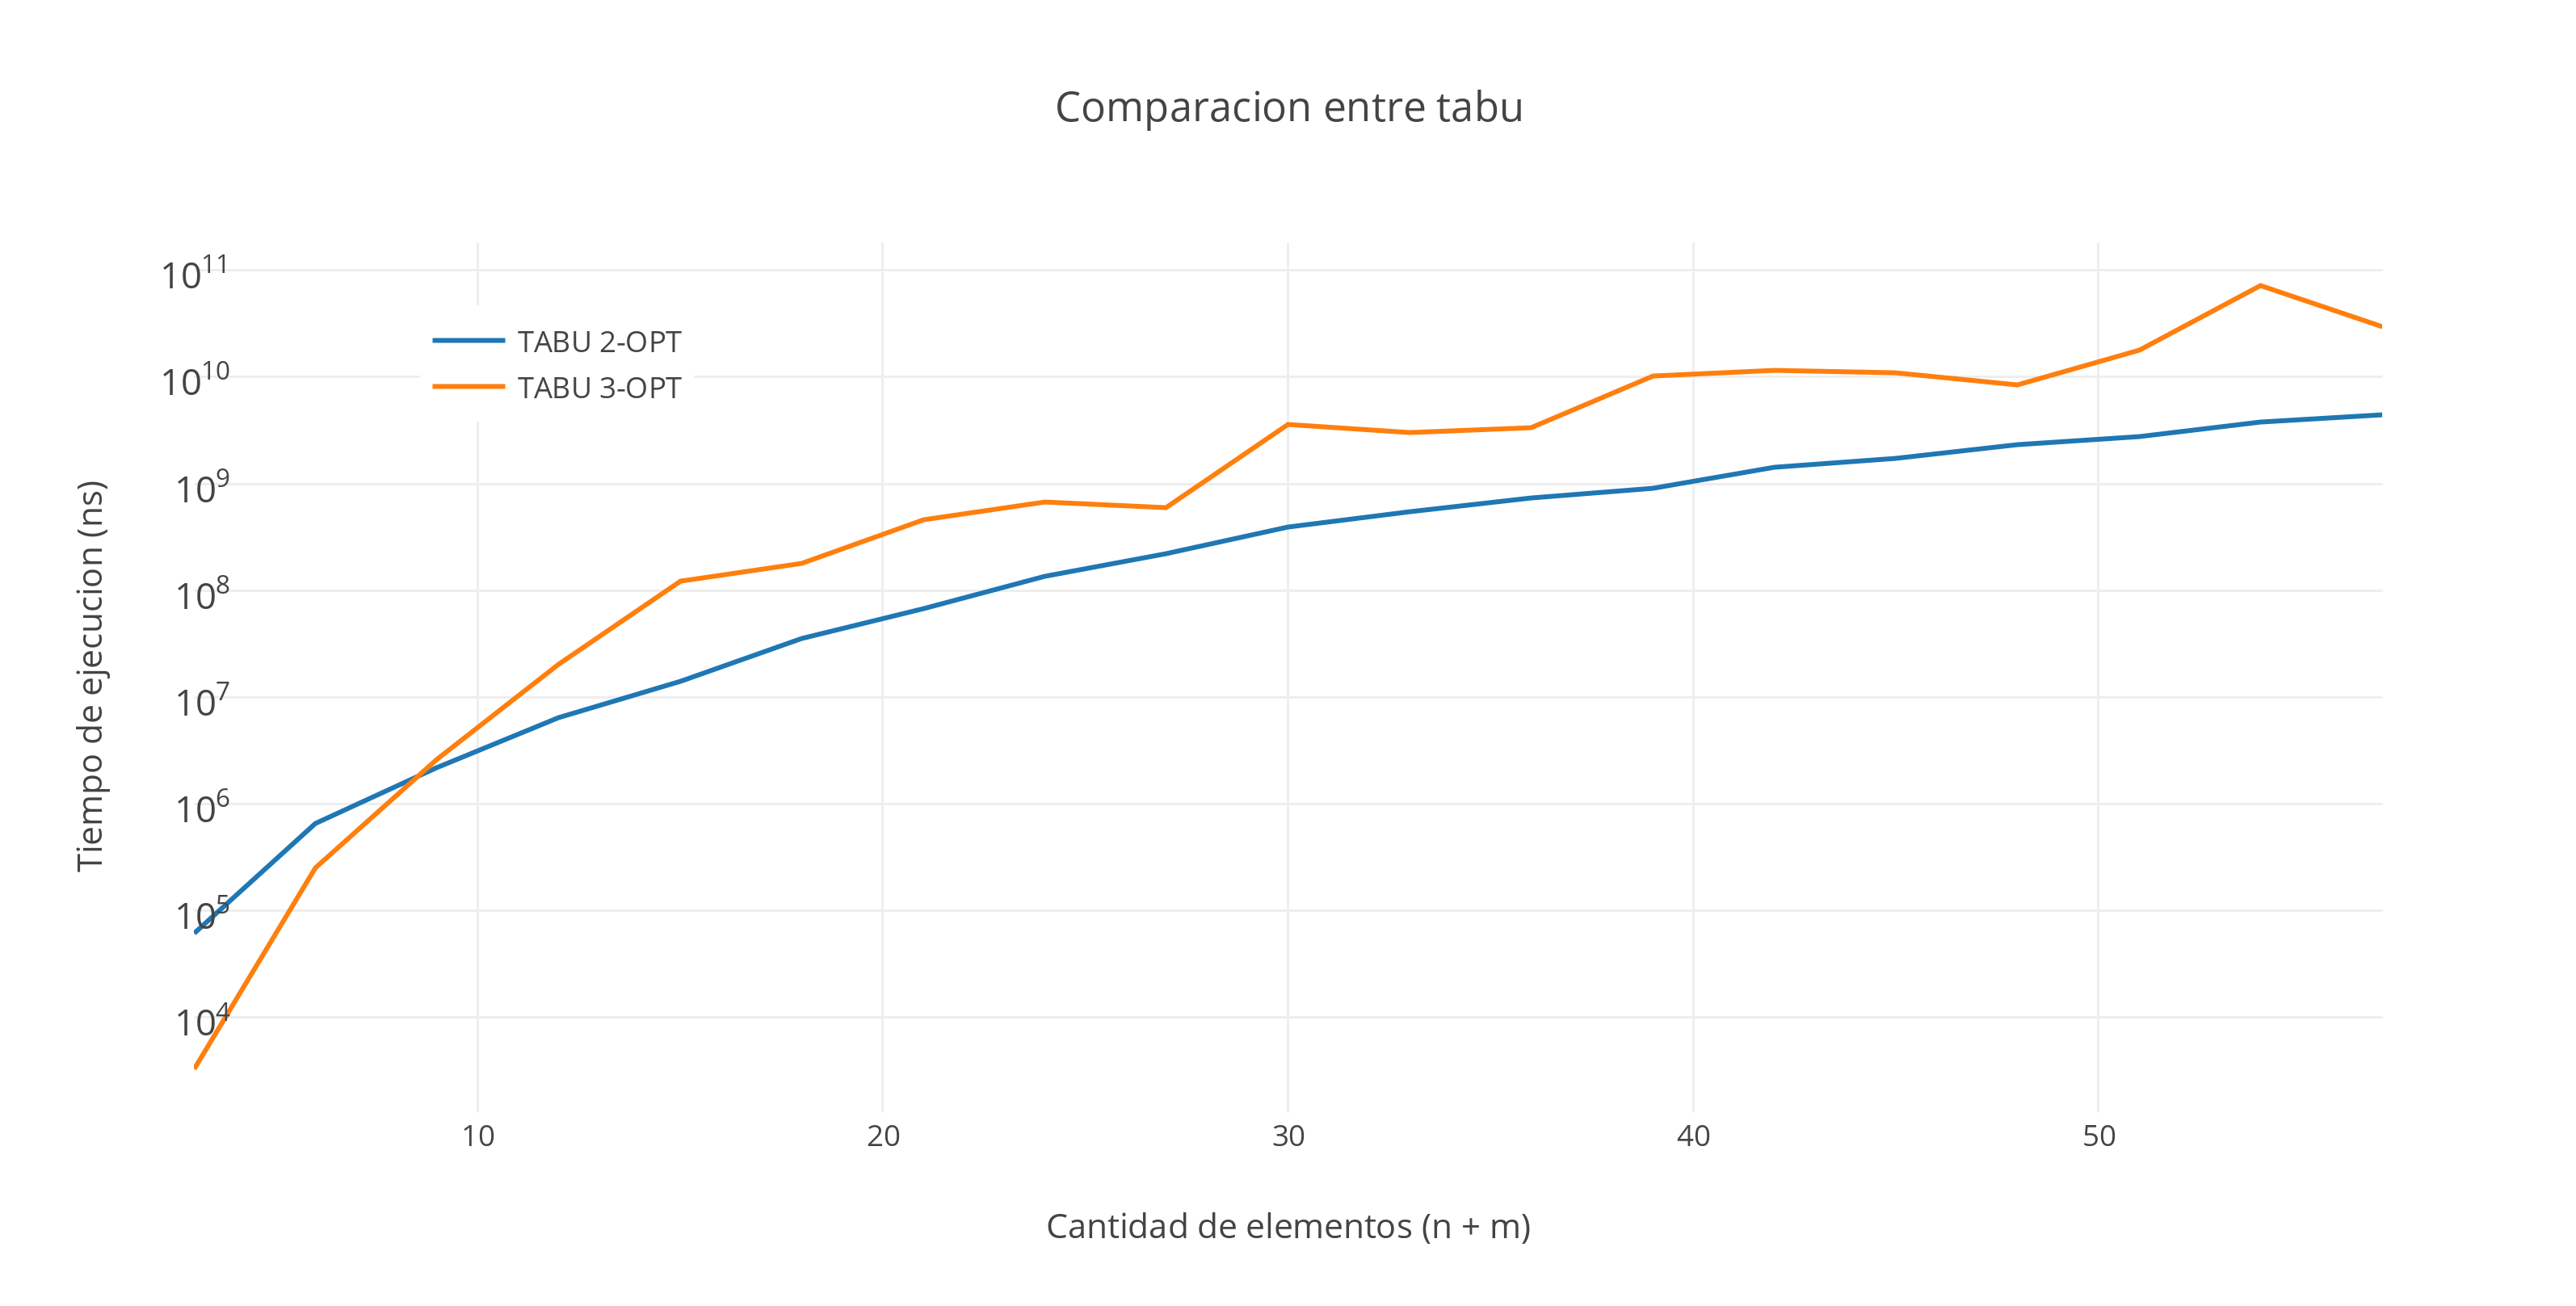
\includegraphics[scale=0.5]{./EJ4/comparacionsinorden1.png}\\
 {            \textit{Gráfico \ 4.12 - Tabu 2-OPT vs Tabu 3-OPT sobre Familia 6}}
  \end{center}
  \vspace*{0.3cm}
  
--> OBTENER CONCLUSIONES

\subsubsection*{Familia 7}

--> PRESENTAR FAMILIA

\vspace*{0.3cm} \vspace*{0.3cm}
  \begin{center}
 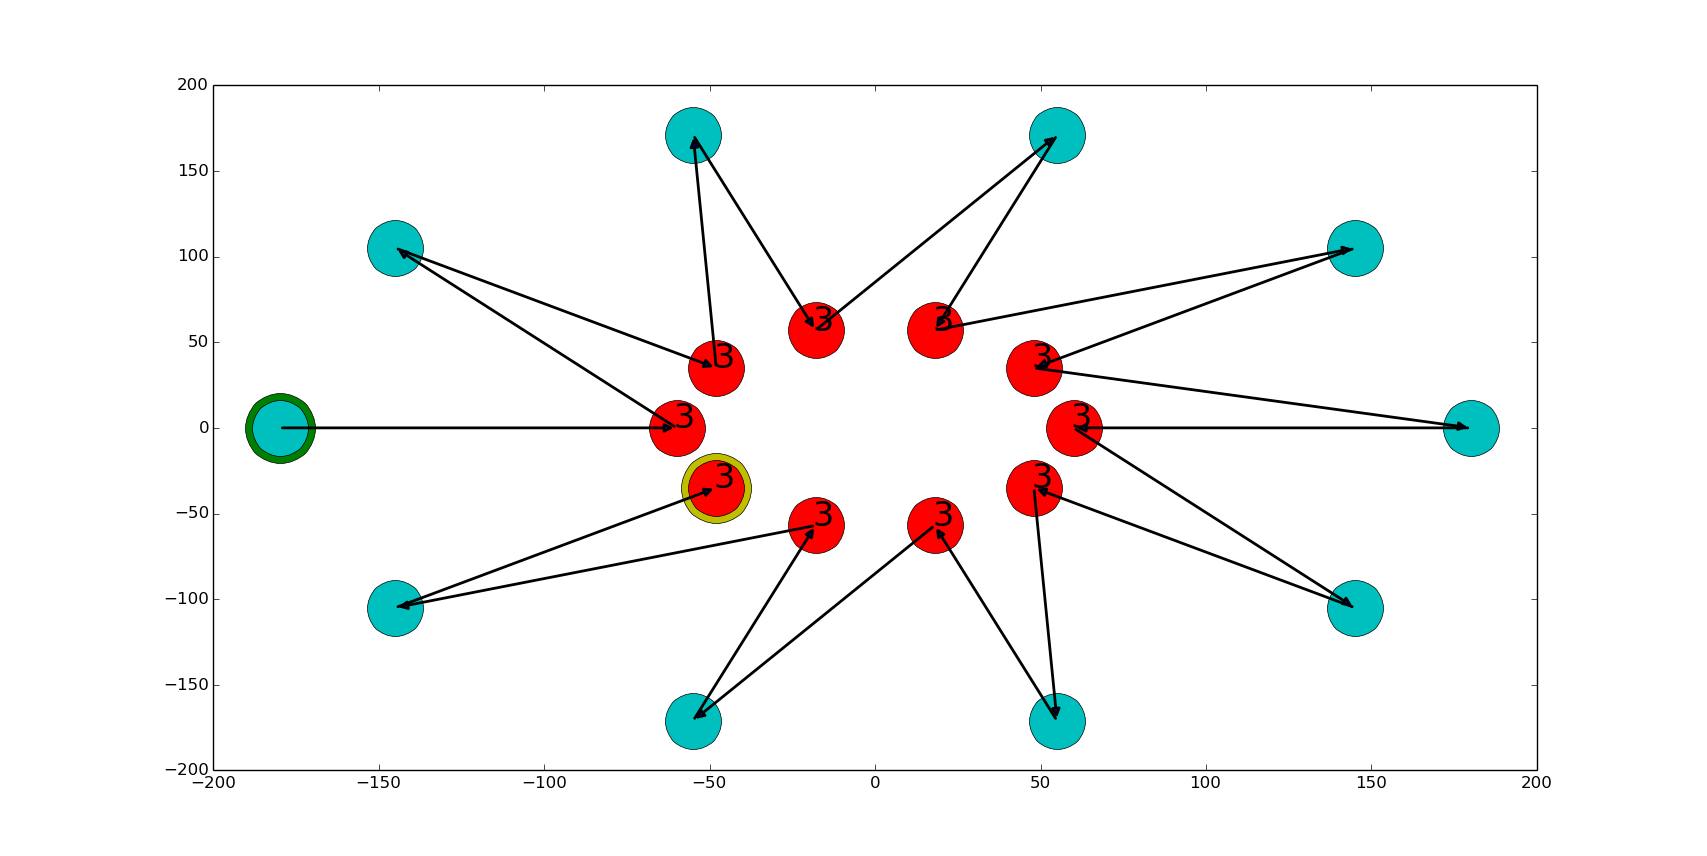
\includegraphics[scale=0.3]{./EJ4/fam7goloso.png}\\
 {            \textit{Soluci\'on Golosa}}
  \end{center}
  \vspace*{0.3cm}

\vspace*{0.3cm} \vspace*{0.3cm}
  \begin{center}
 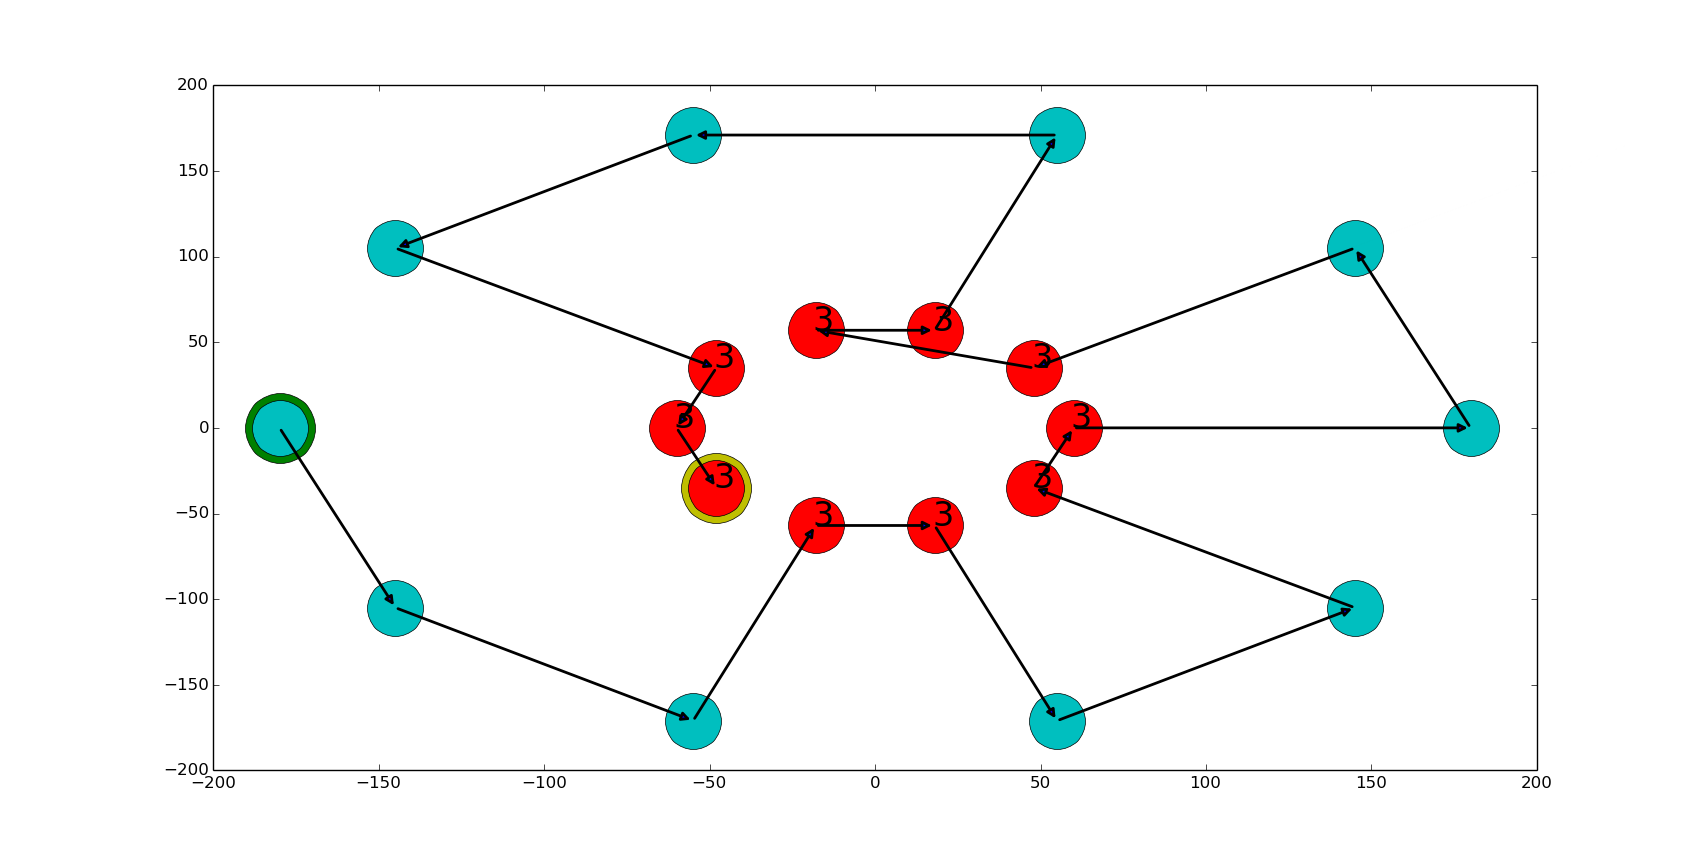
\includegraphics[scale=0.3]{./EJ4/fam72opt.png}\\
 {            \textit{Soluci\'on TABU 2-OPT}}
  \end{center}
  \vspace*{0.3cm}

\vspace*{0.3cm} \vspace*{0.3cm}
  \begin{center}
 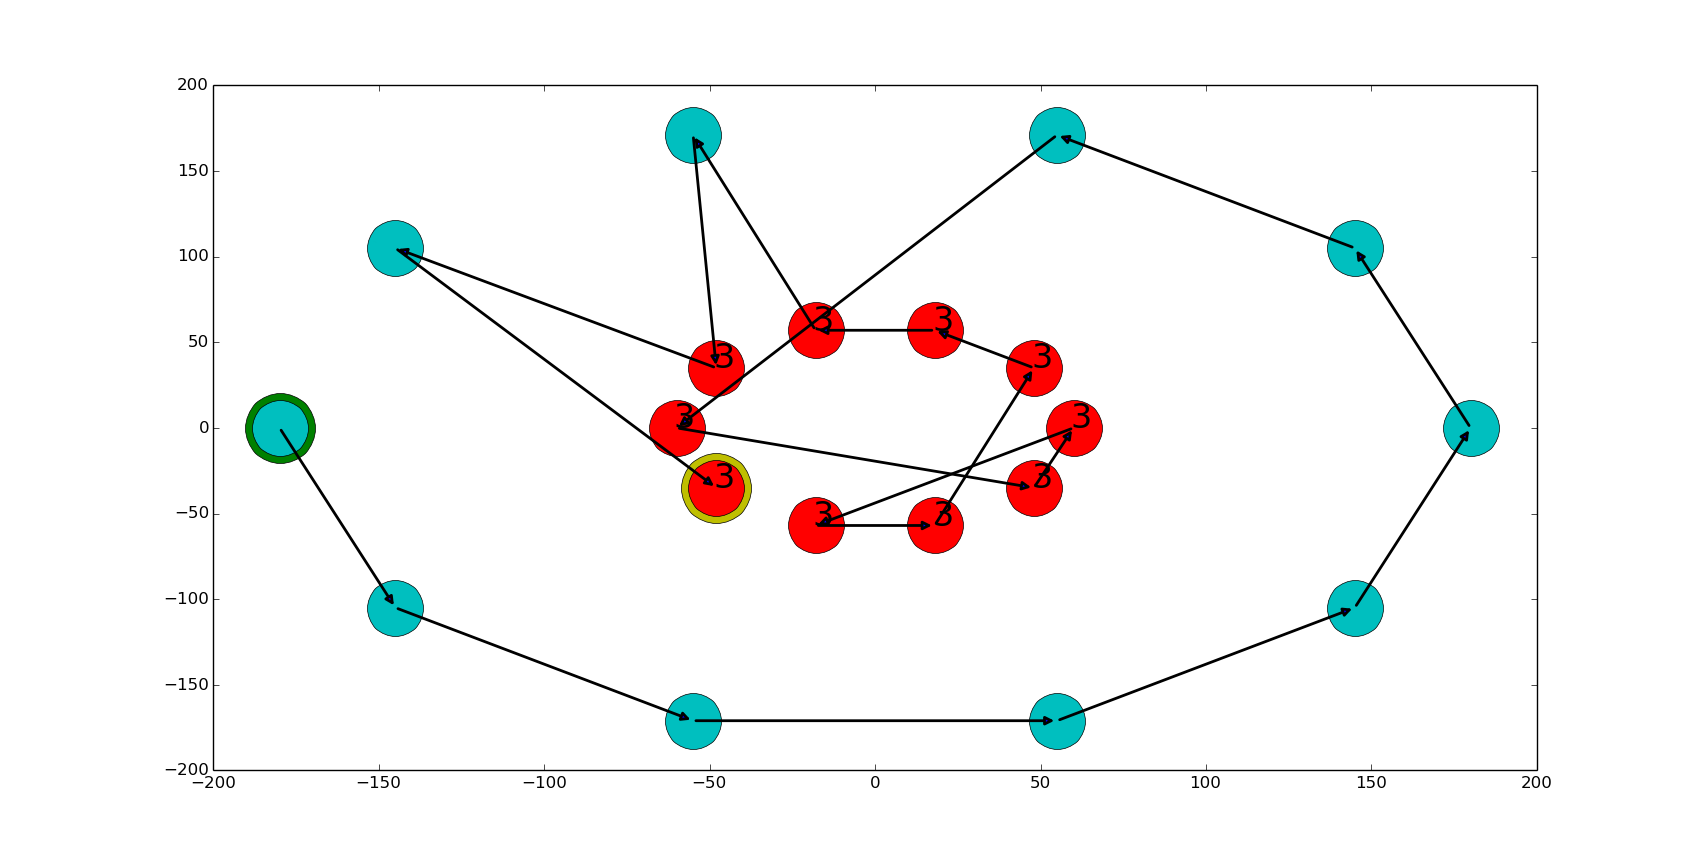
\includegraphics[scale=0.3]{./EJ4/fam73opt.png}\\
 {            \textit{Soluci\'on TABU 3-OPT}}
  \end{center}
  \vspace*{0.3cm}

Veamos como se comporta Tabu 2-OPT con respecto a la heuristica de busqueda local 2-OPT:

\vspace*{0.3cm} \vspace*{0.3cm}
  \begin{center}
 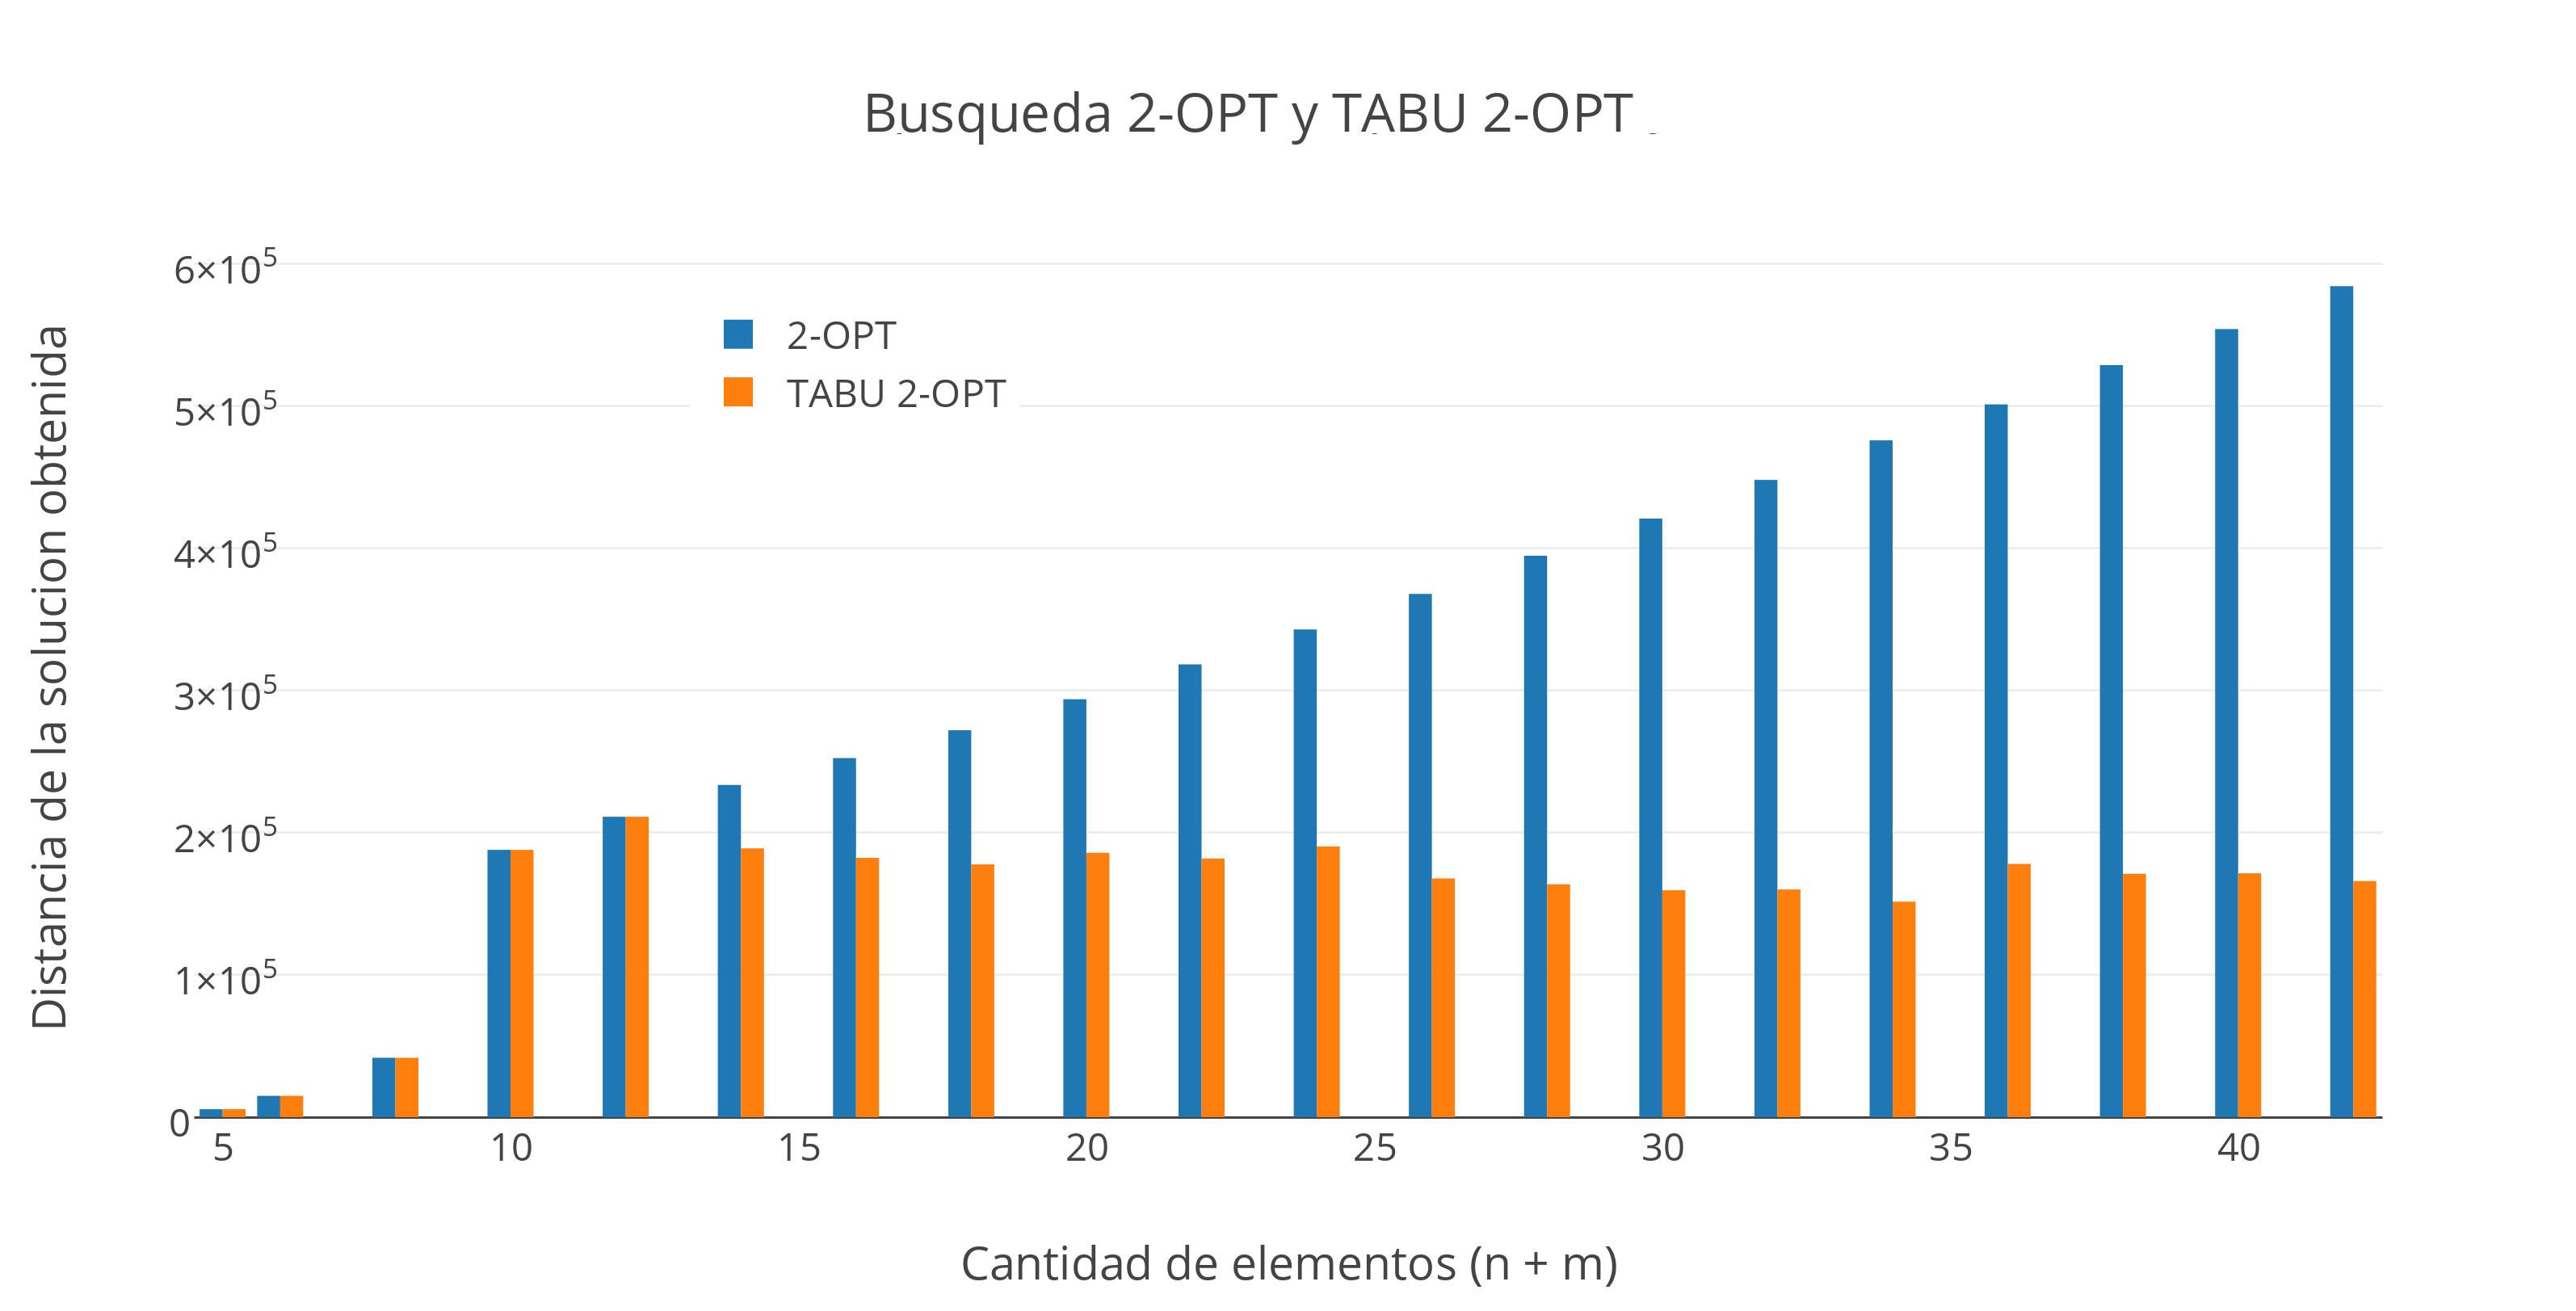
\includegraphics[scale=0.5]{./EJ4/comparativoanillos2opt.png}\\
 {            \textit{Gráfico \ 4.7 - 2-OPT vs Tabu 2-OPT sobre Familia 7}}
  \end{center}
  \vspace*{0.3cm}

\vspace*{0.3cm} \vspace*{0.3cm}
  \begin{center}
 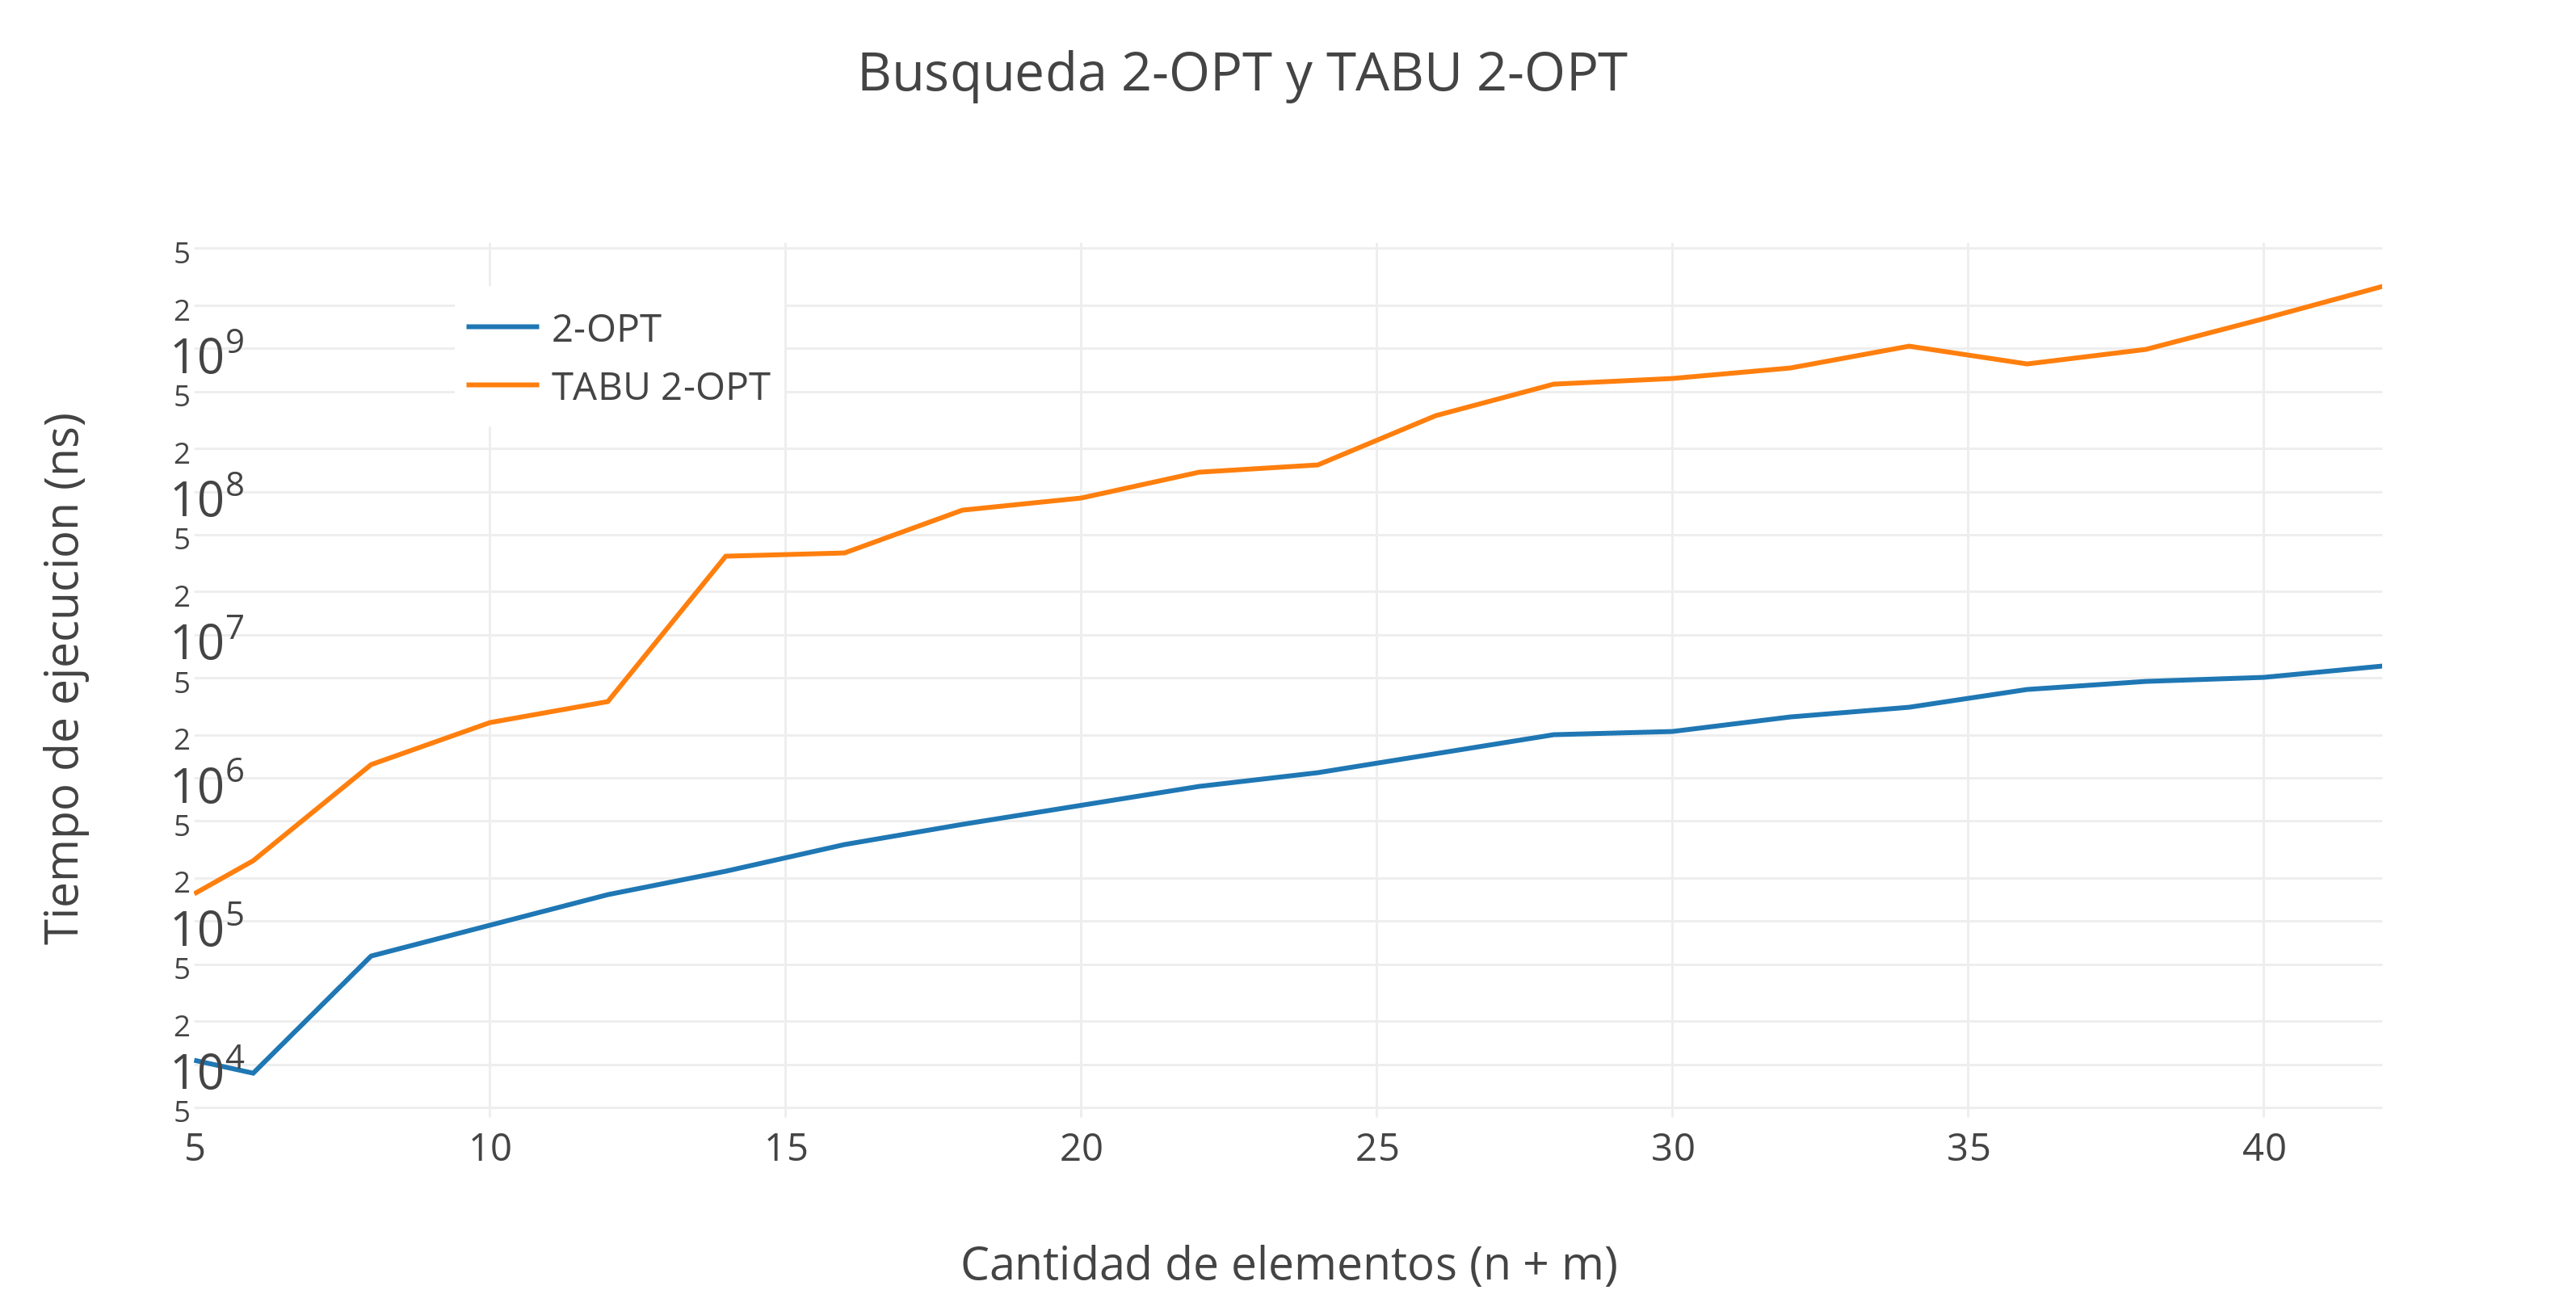
\includegraphics[scale=0.5]{./EJ4/medicionanillos2opt.png}\\
 {            \textit{Gráfico \ 4.8 - 2-OPT vs Tabu 2-OPT sobre Familia 7}}
  \end{center}
  \vspace*{0.3cm}

Luego, para 3-OPT:

\vspace*{0.3cm} \vspace*{0.3cm}
  \begin{center}
 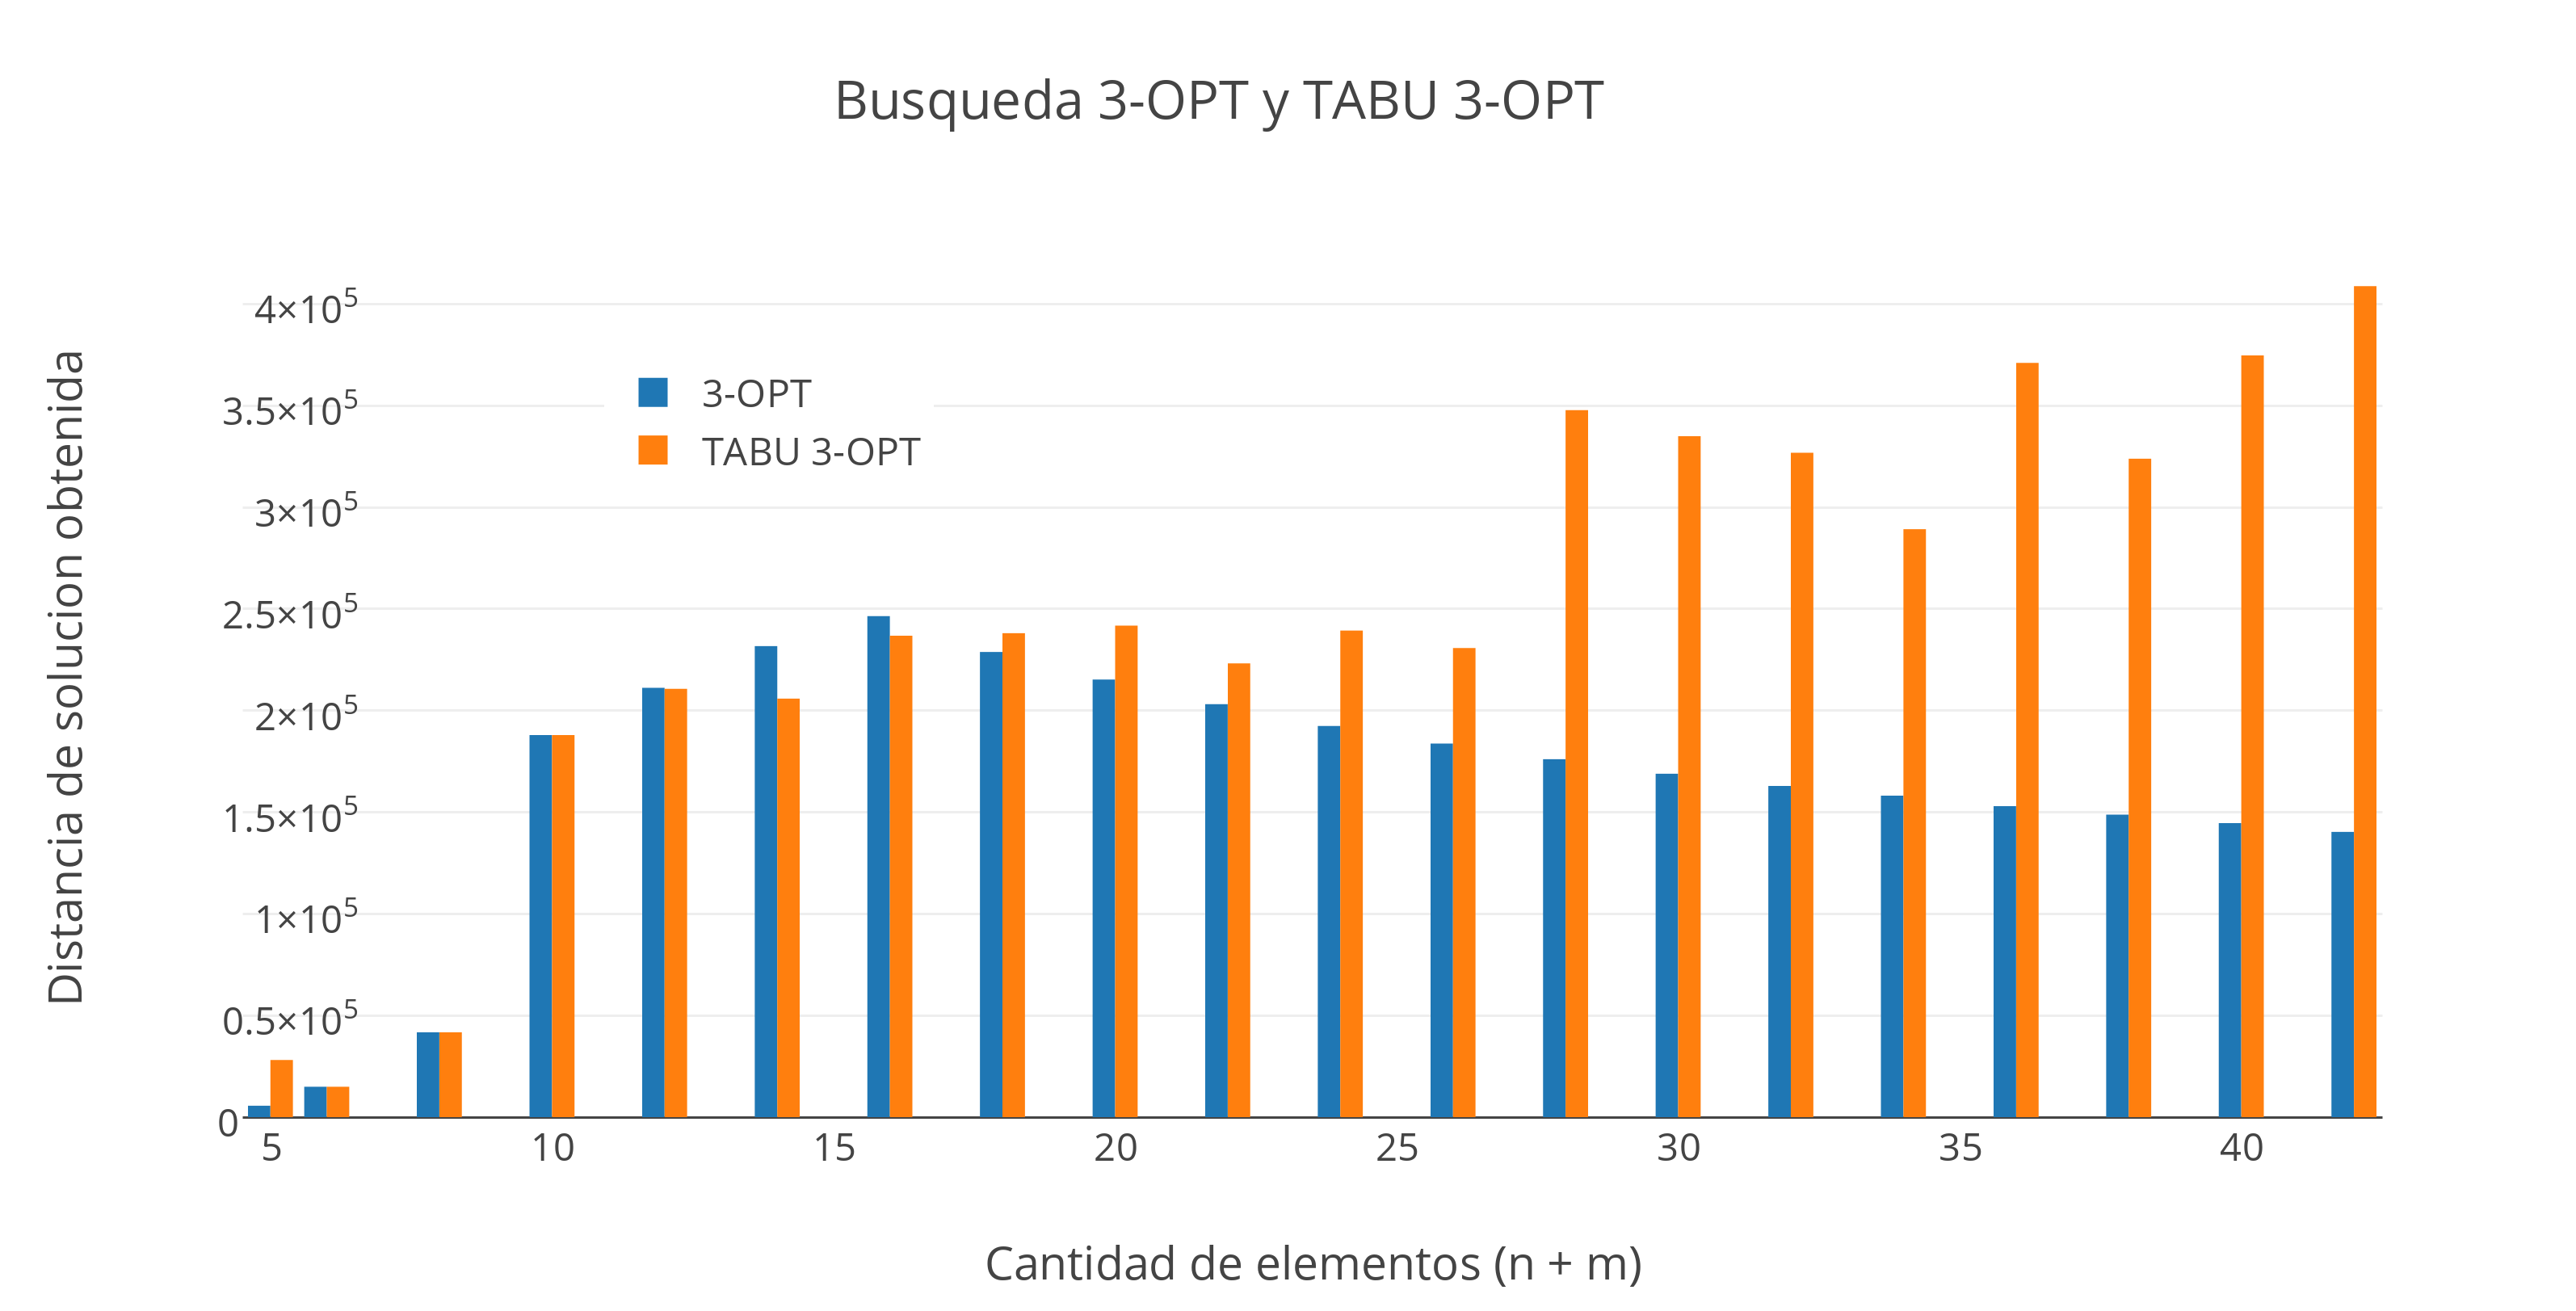
\includegraphics[scale=0.5]{./EJ4/comparativoanillos3opt.png}\\
 {            \textit{Gráfico \ 4.9 - 3-OPT vs Tabu 3-OPT sobre Familia 7}}
  \end{center}
  \vspace*{0.3cm}

\vspace*{0.3cm} \vspace*{0.3cm}
  \begin{center}
 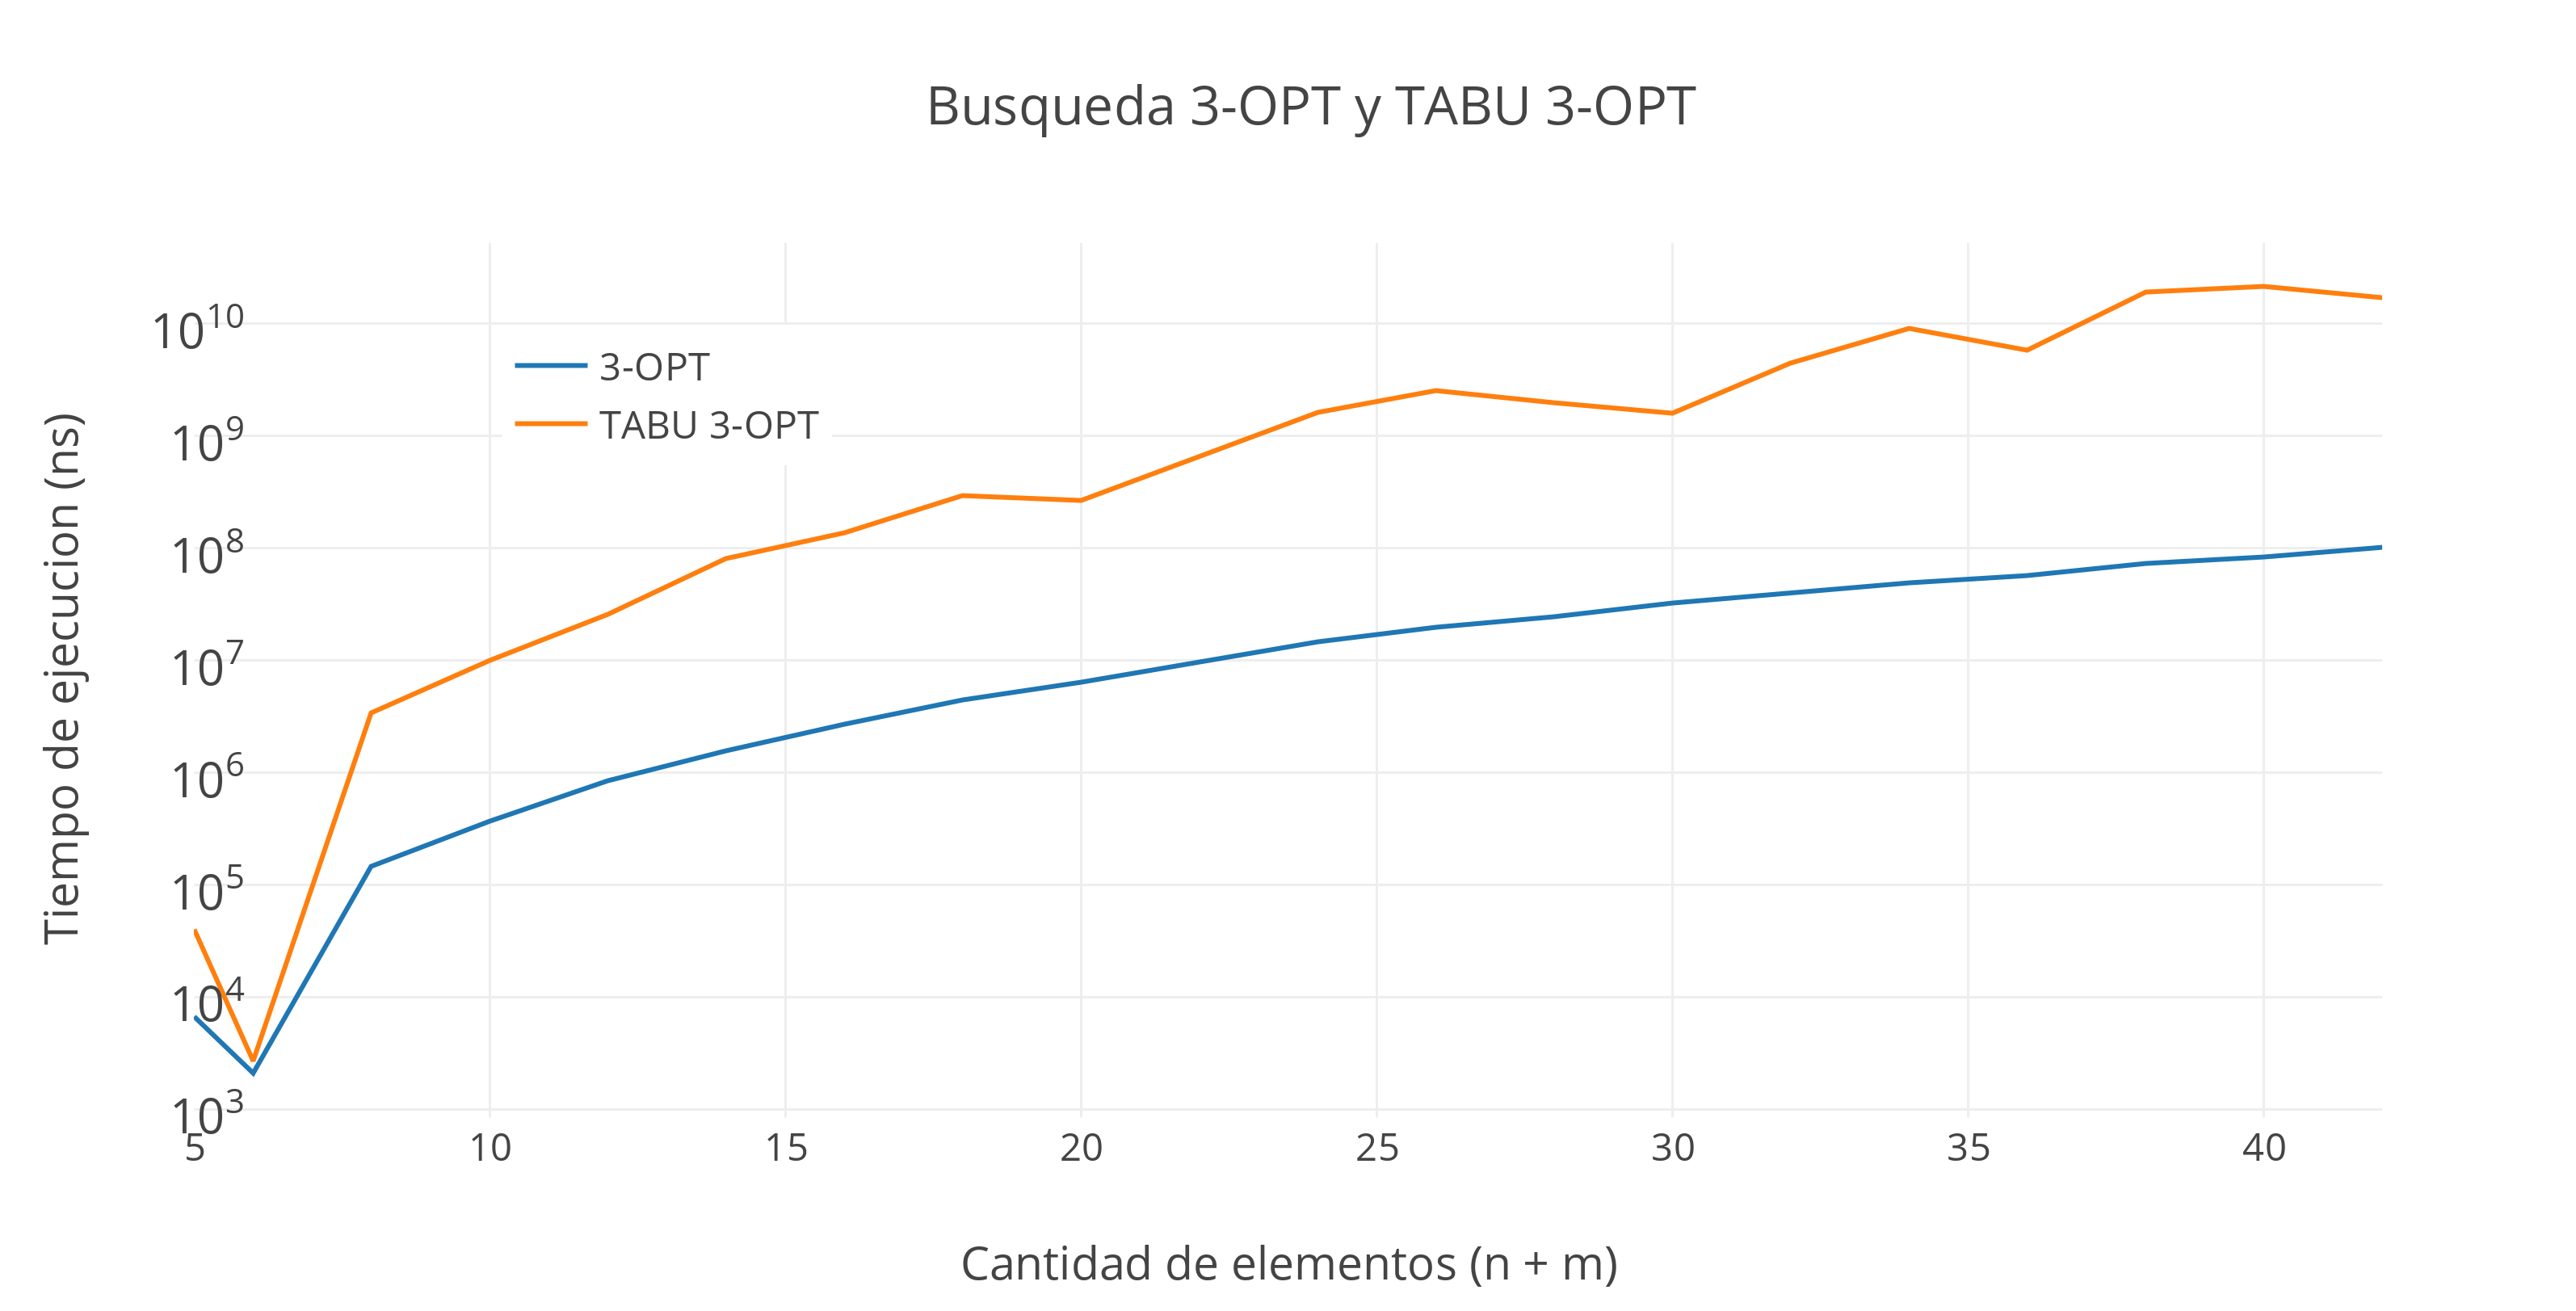
\includegraphics[scale=0.5]{./EJ4/medicionanillos3opt.png}\\
 {            \textit{Gráfico \ 4.10 - 3-OPT vs Tabu 3-OPT sobre Familia 7}}
  \end{center}
  \vspace*{0.3cm}
  
--> OBTENER CONCLUSIONES  
 
Comparando las soluciones de cada version de tabú search podemos observar lo siguiente: 
  
\vspace*{0.3cm} \vspace*{0.3cm}
  \begin{center}
 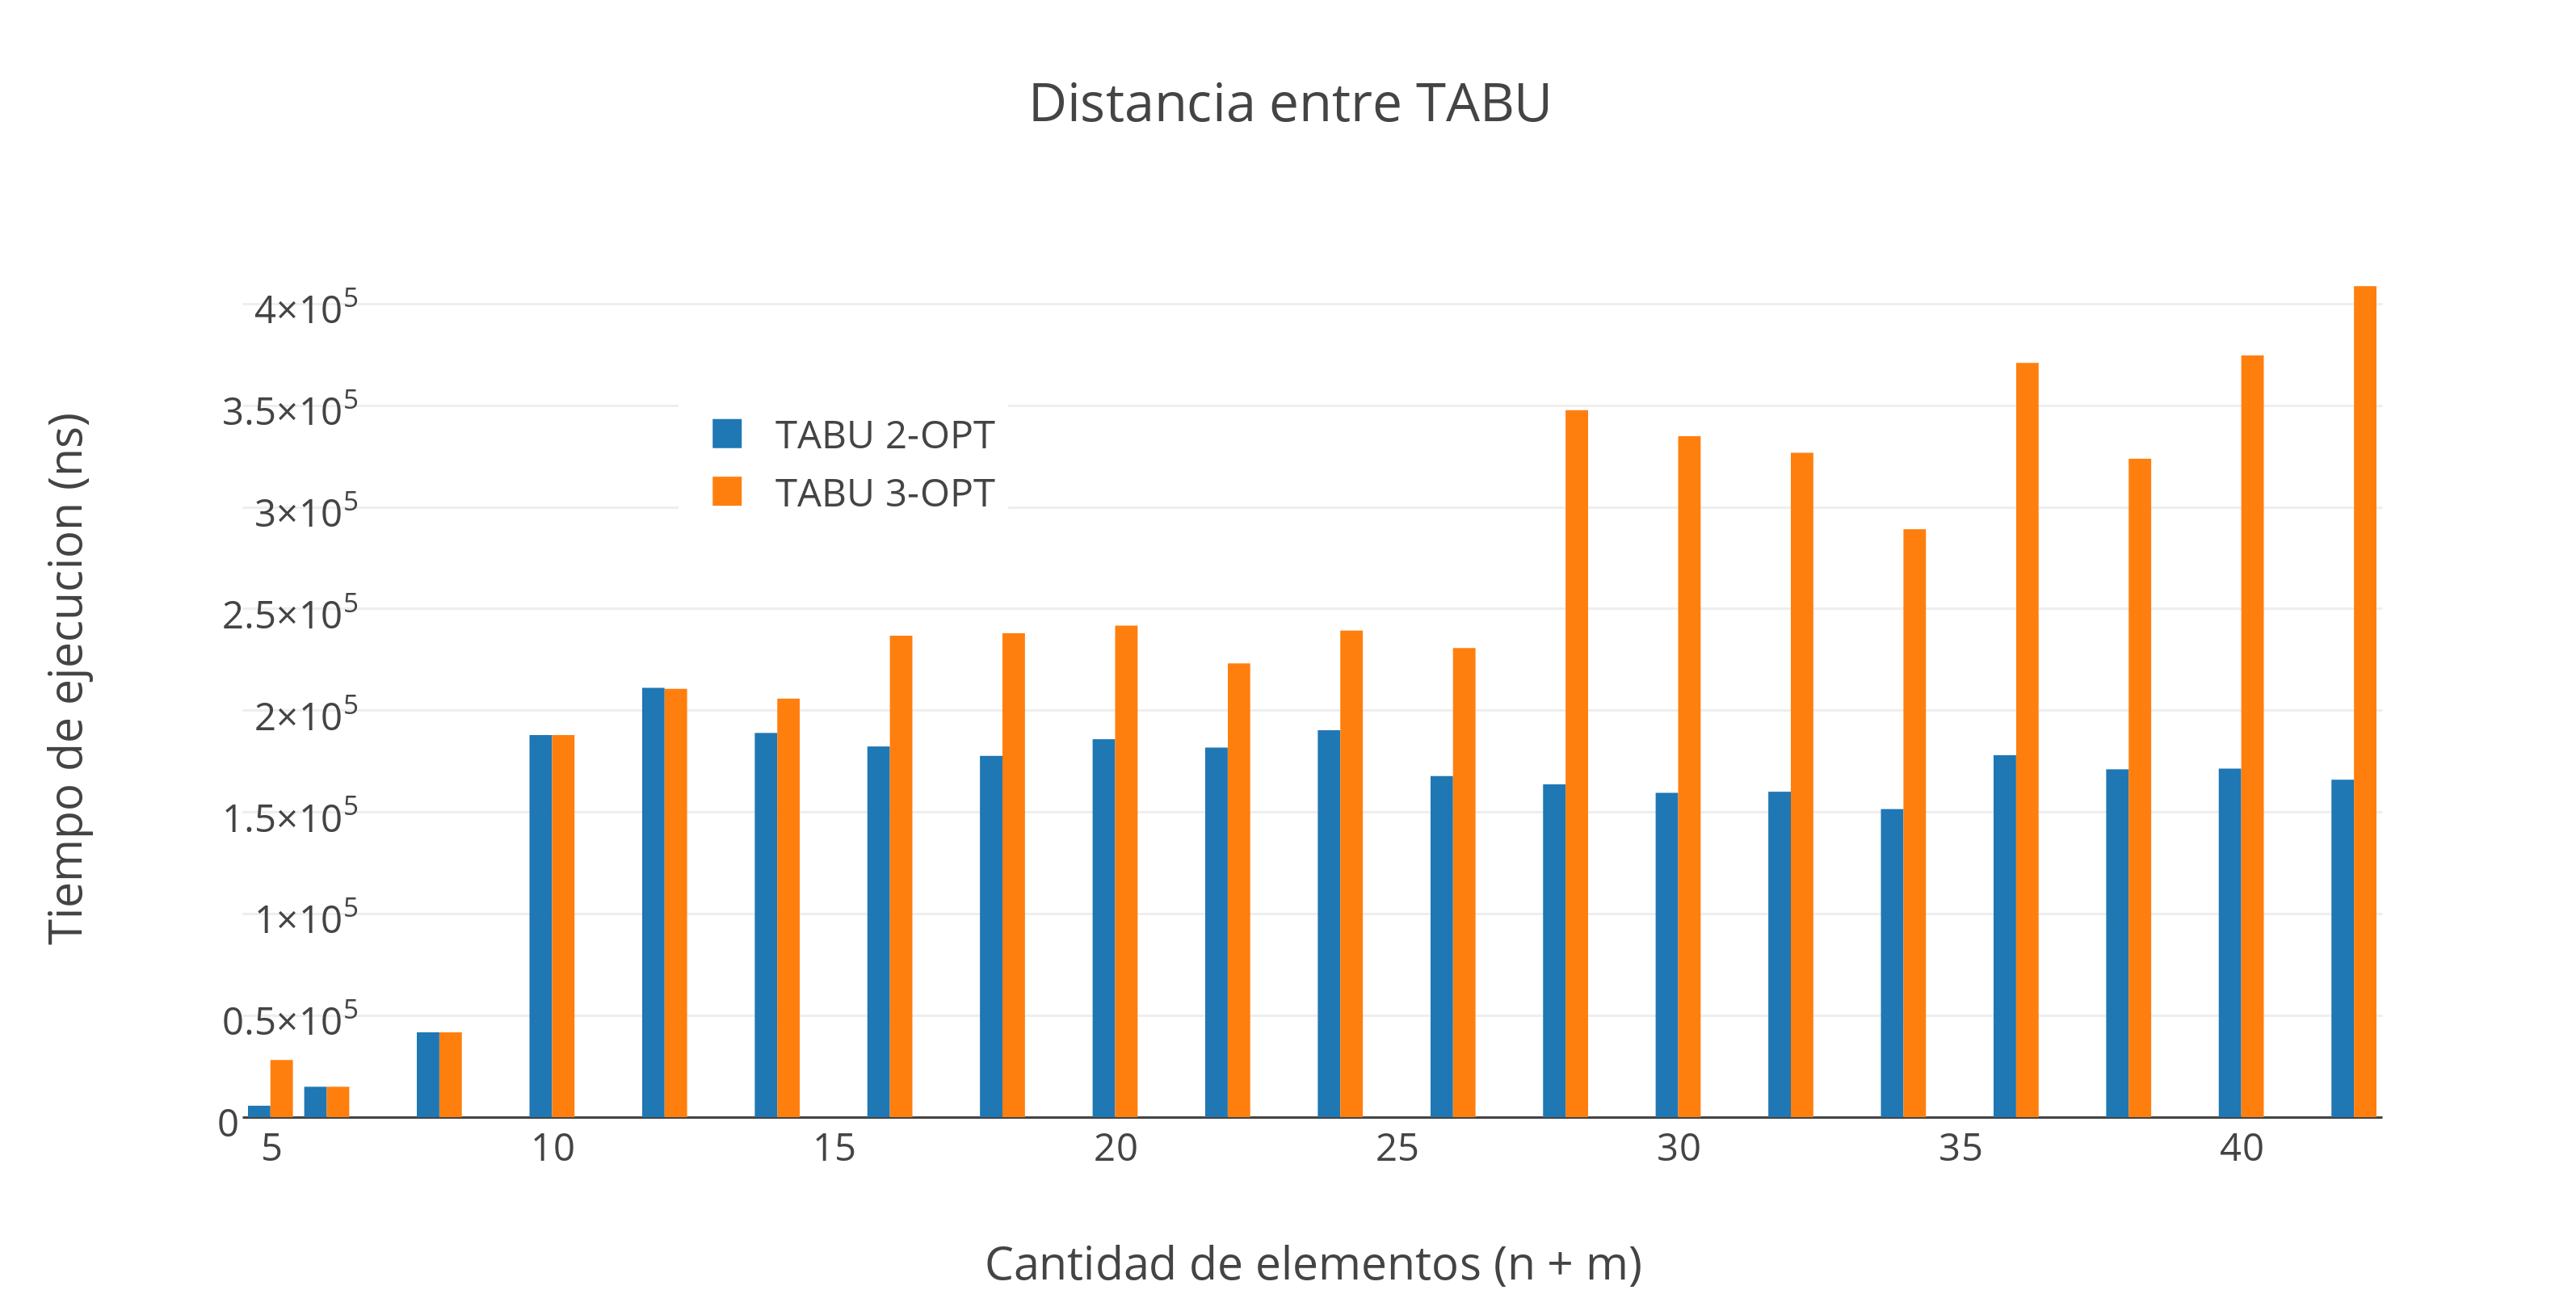
\includegraphics[scale=0.5]{./EJ4/comparativoanillos1.png}\\
 {            \textit{Gráfico \ 4.11 - Tabu 2-OPT vs Tabu 3-OPT sobre Familia 7}}
  \end{center}
  \vspace*{0.3cm}

\vspace*{0.3cm} \vspace*{0.3cm}
  \begin{center}
 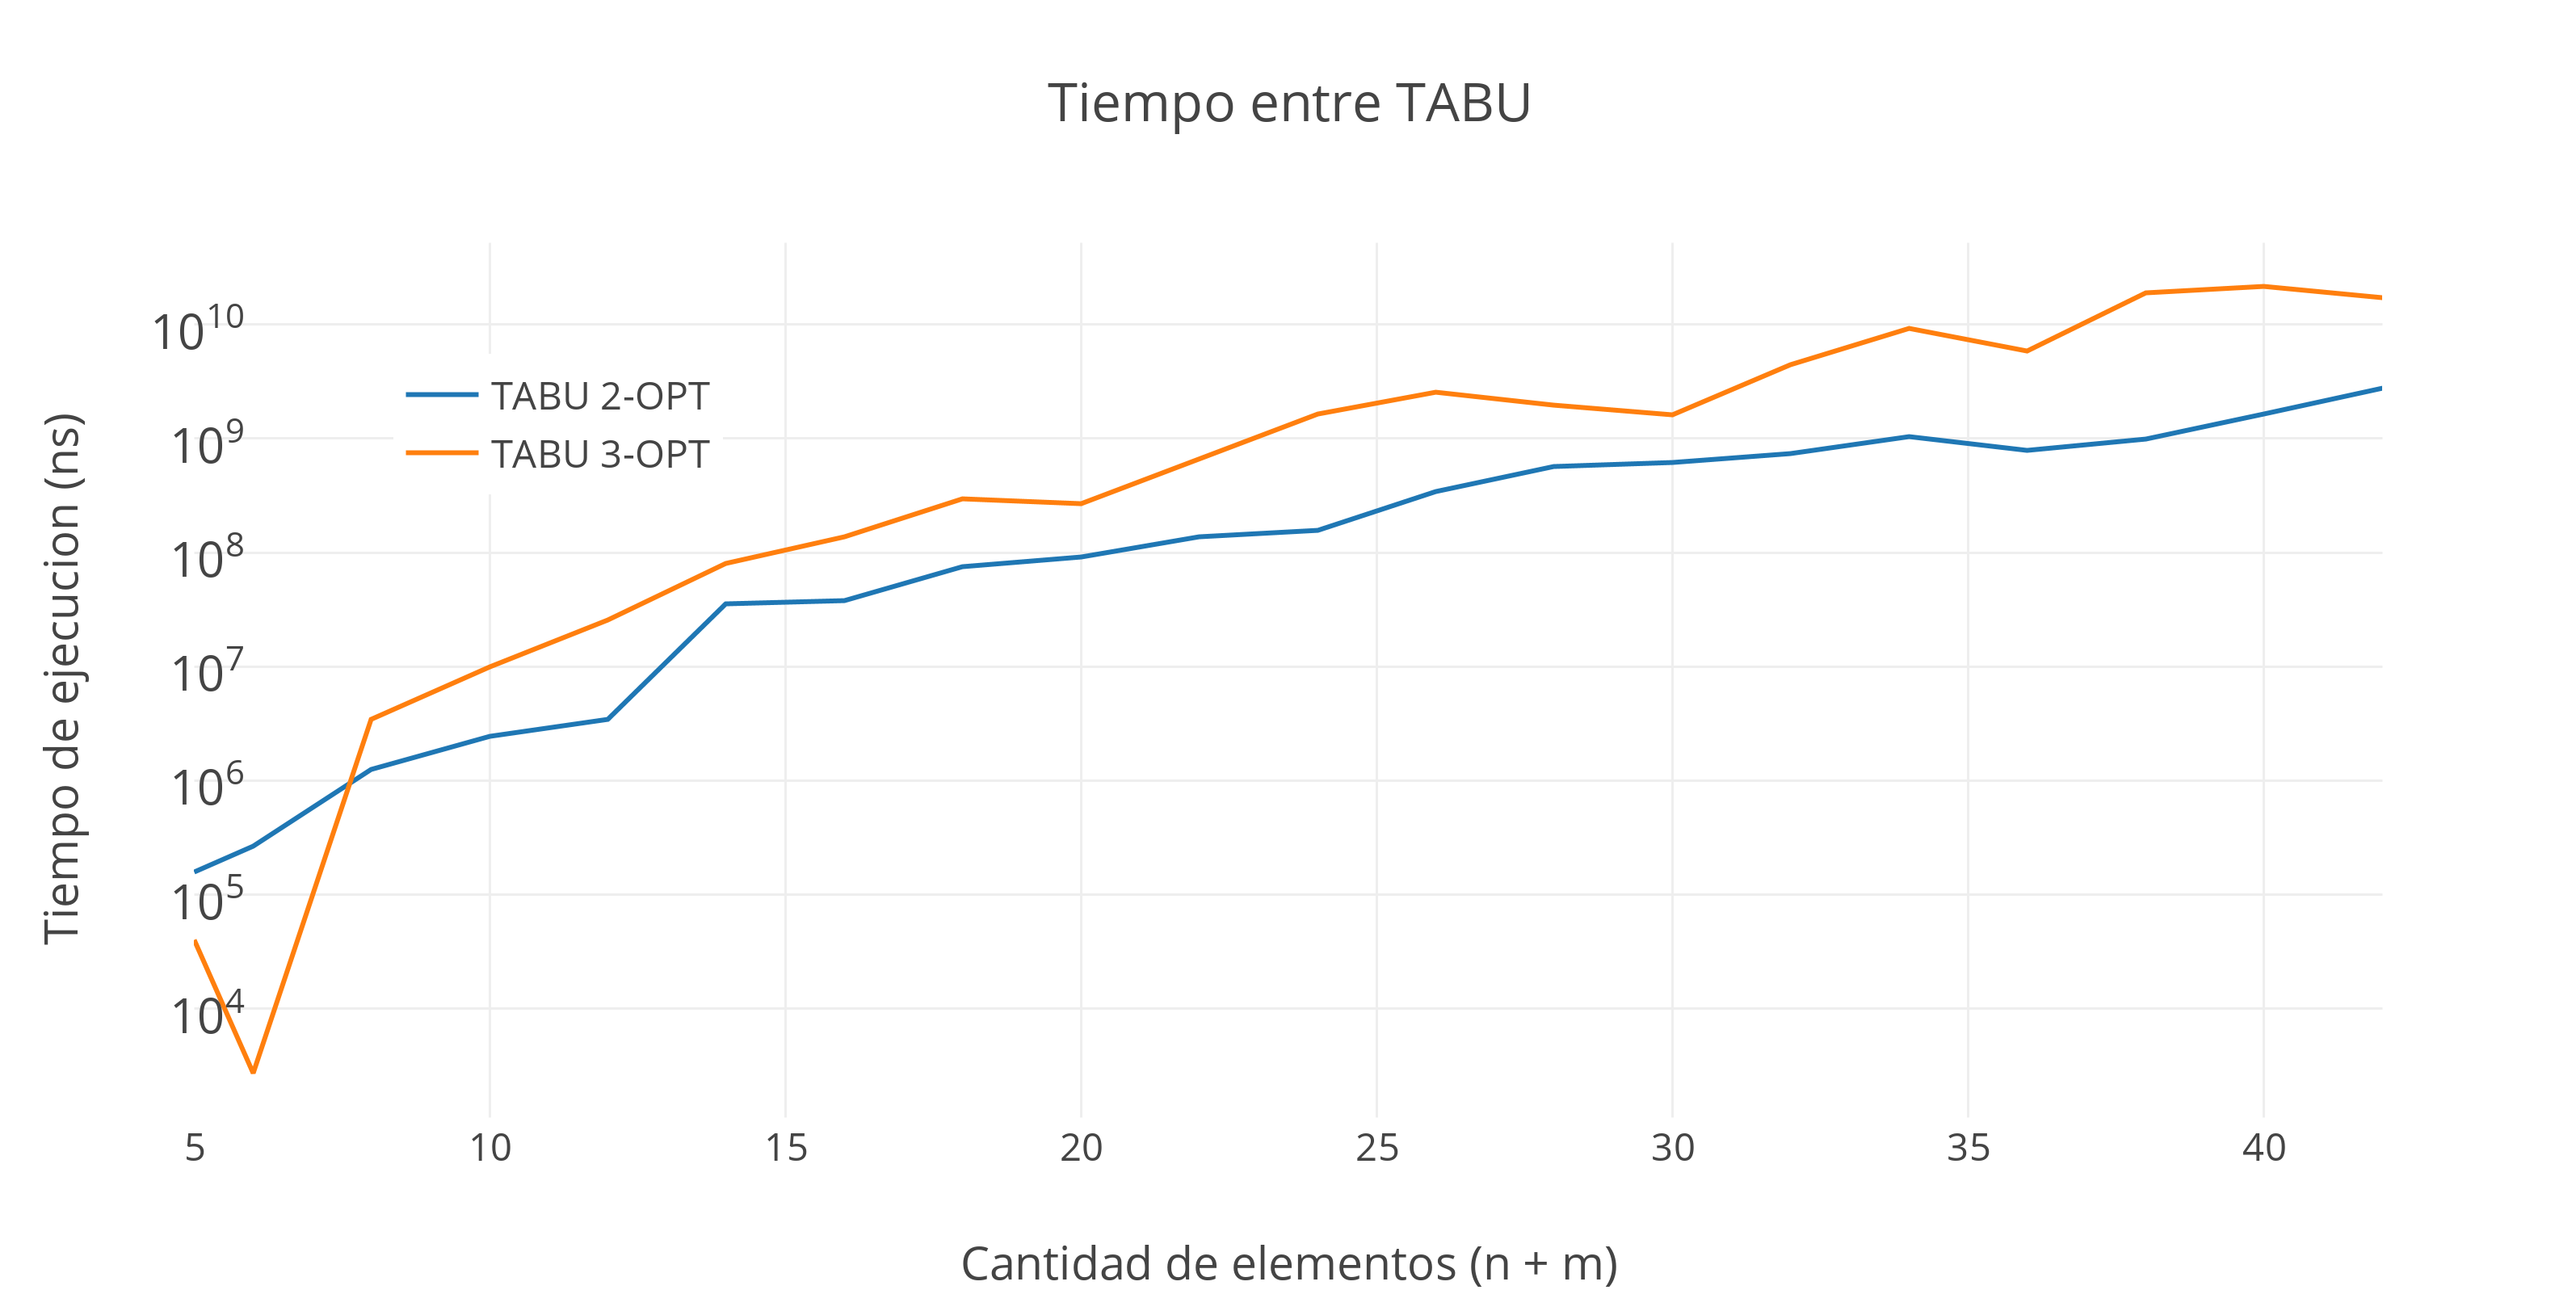
\includegraphics[scale=0.5]{./EJ4/comparativoanillos.png}\\
 {            \textit{Gráfico \ 4.12 - Tabu 2-OPT vs Tabu 3-OPT sobre Familia 7}}
  \end{center}
  \vspace*{0.3cm}

\subsubsection*{Familia 8}

--> PRESENTAR FAMILIA

\vspace*{0.3cm} \vspace*{0.3cm}
  \begin{center}
 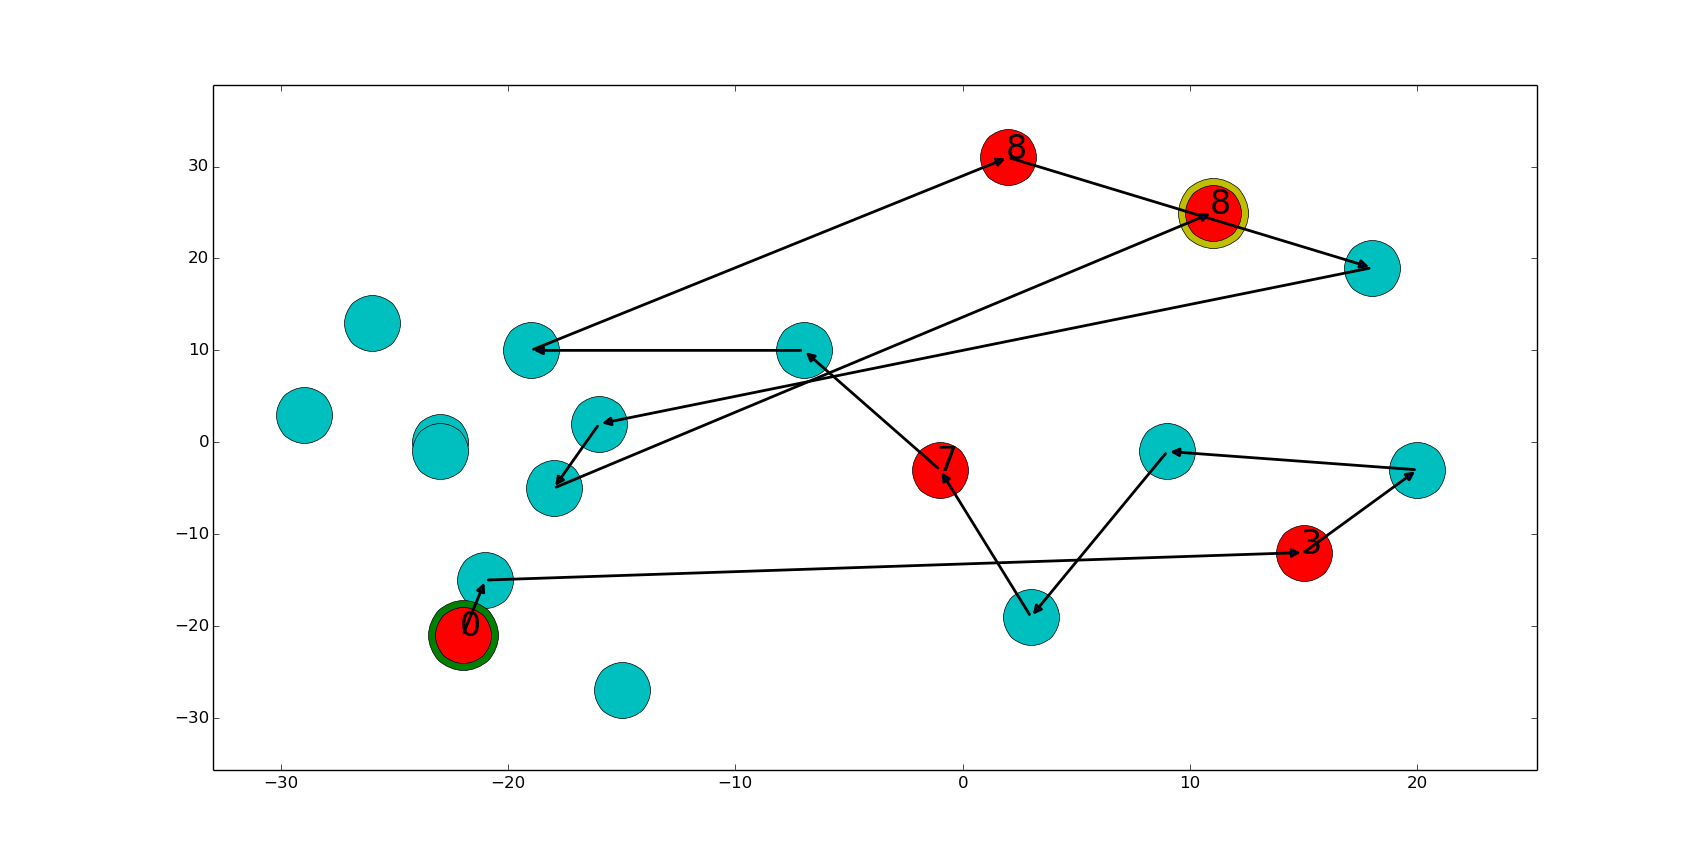
\includegraphics[scale=0.3]{./EJ4/fam8goloso.png}\\
 {            \textit{Soluci\'on Golosa}}
  \end{center}
  \vspace*{0.3cm}

\vspace*{0.3cm} \vspace*{0.3cm}
  \begin{center}
 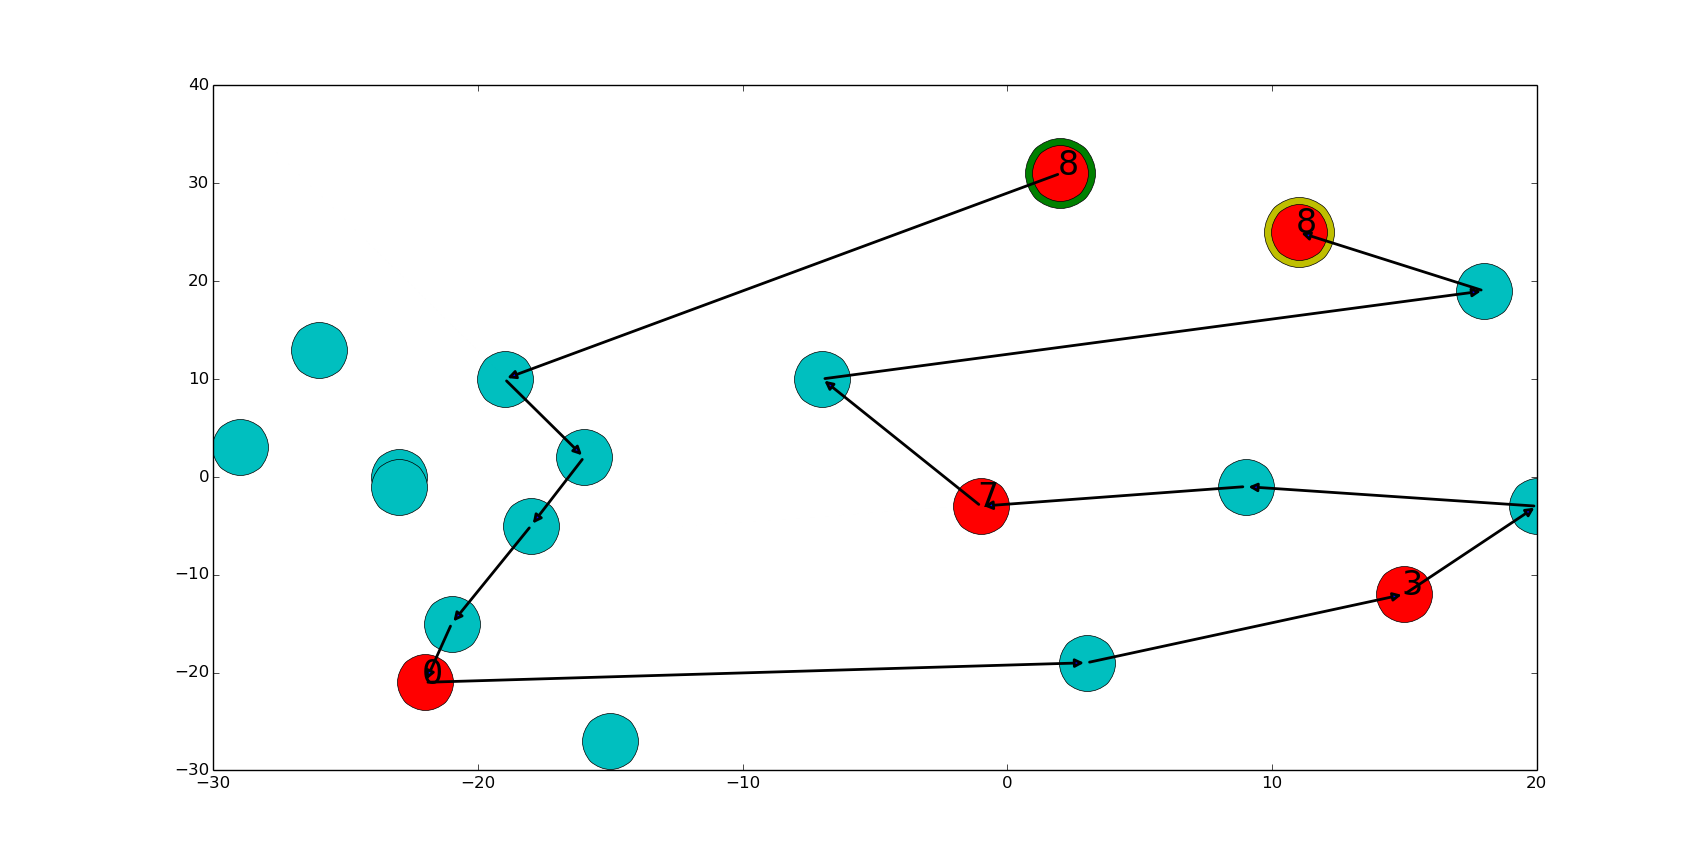
\includegraphics[scale=0.3]{./EJ4/fam82opt.png}\\
 {            \textit{Soluci\'on TABU 2-OPT}}
  \end{center}
  \vspace*{0.3cm}

\vspace*{0.3cm} \vspace*{0.3cm}
  \begin{center}
 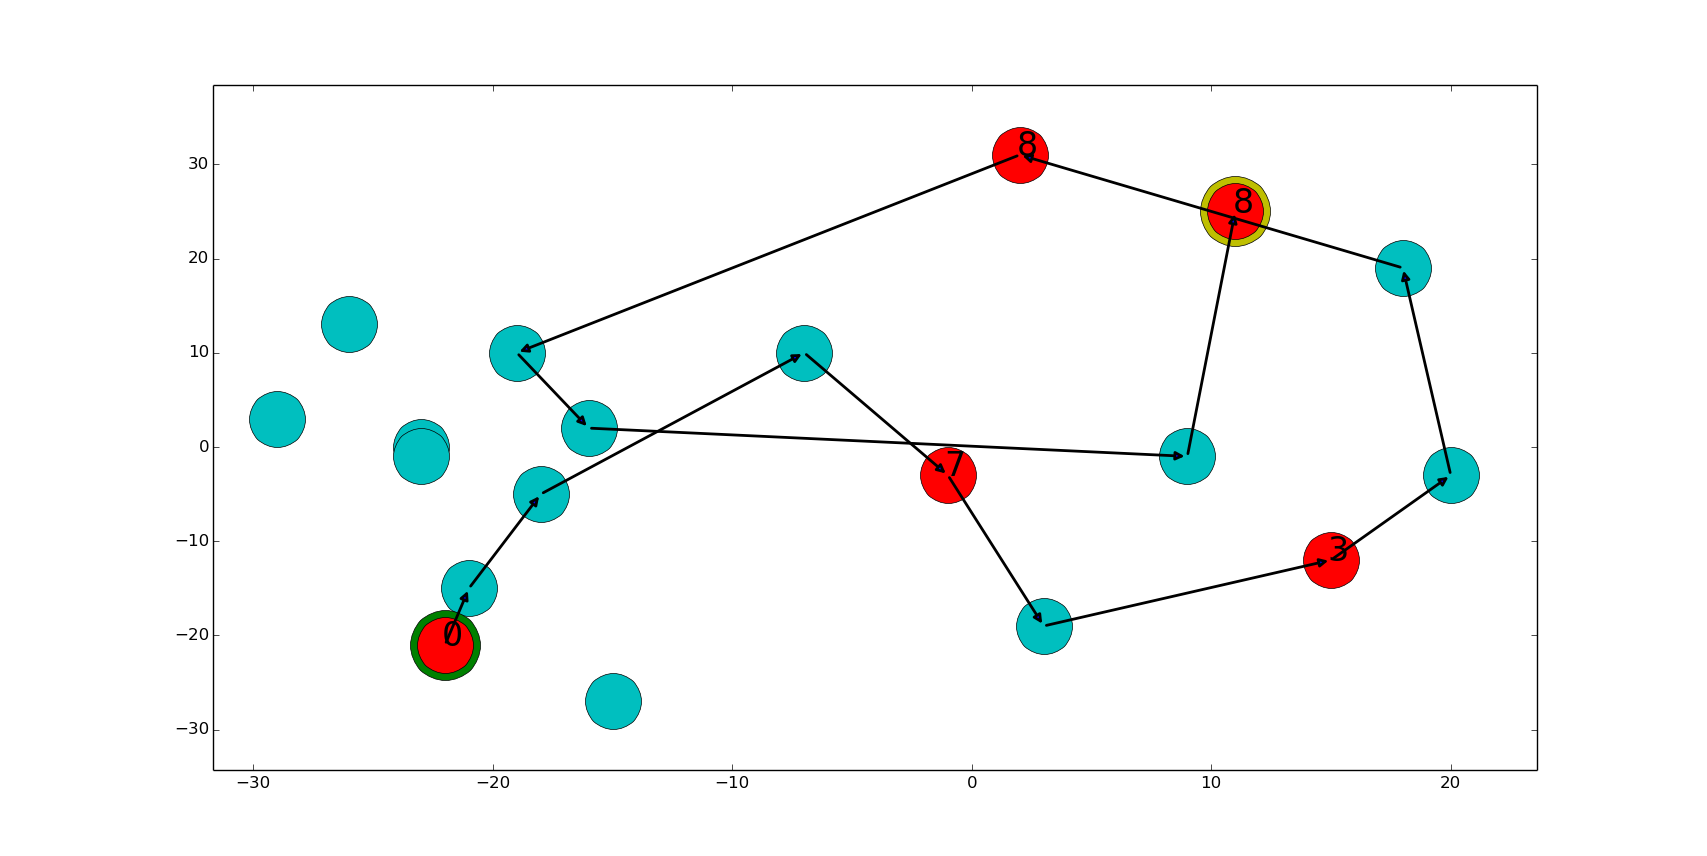
\includegraphics[scale=0.3]{./EJ4/fam83opt.png}\\
 {            \textit{Soluci\'on TABU 3-OPT}}
  \end{center}
  \vspace*{0.3cm}

Veamos como se comporta Tabu 2-OPT con respecto a la heuristica de busqueda local 2-OPT:

\vspace*{0.3cm} \vspace*{0.3cm}
  \begin{center}
 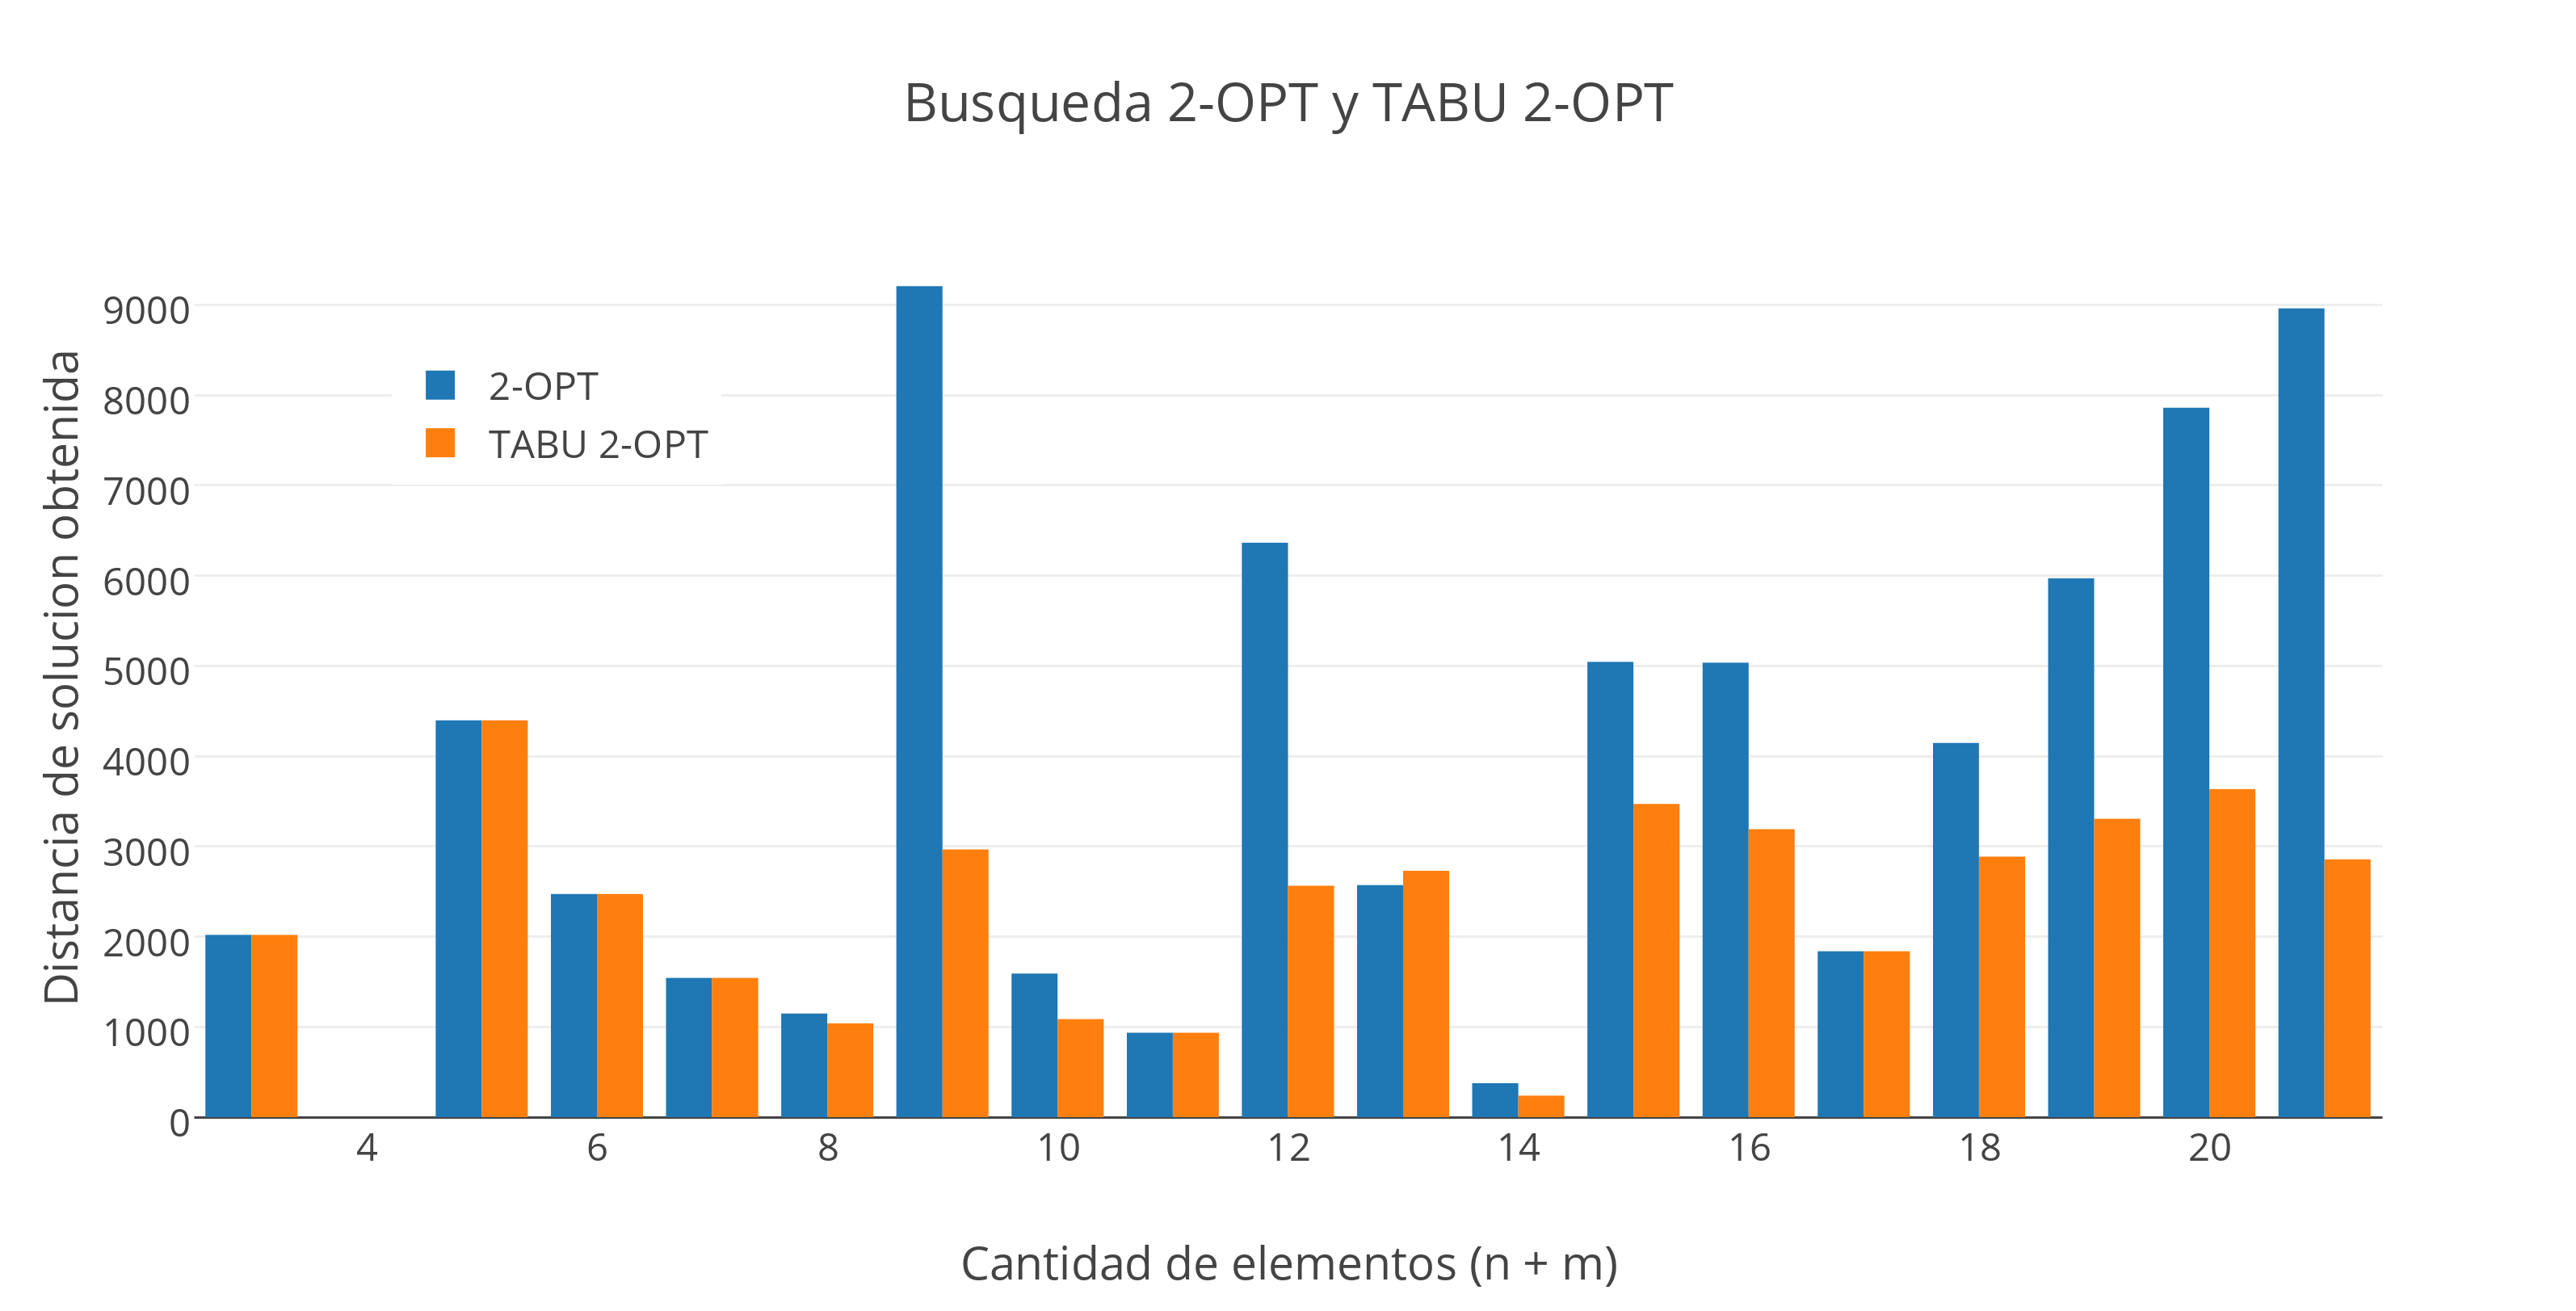
\includegraphics[scale=0.5]{./EJ4/comparativorandom2opt.png}\\
 {            \textit{Gráfico \ 4.7 - 2-OPT vs Tabu 2-OPT sobre Familia 8}}
  \end{center}
  \vspace*{0.3cm}

\vspace*{0.3cm} \vspace*{0.3cm}
  \begin{center}
 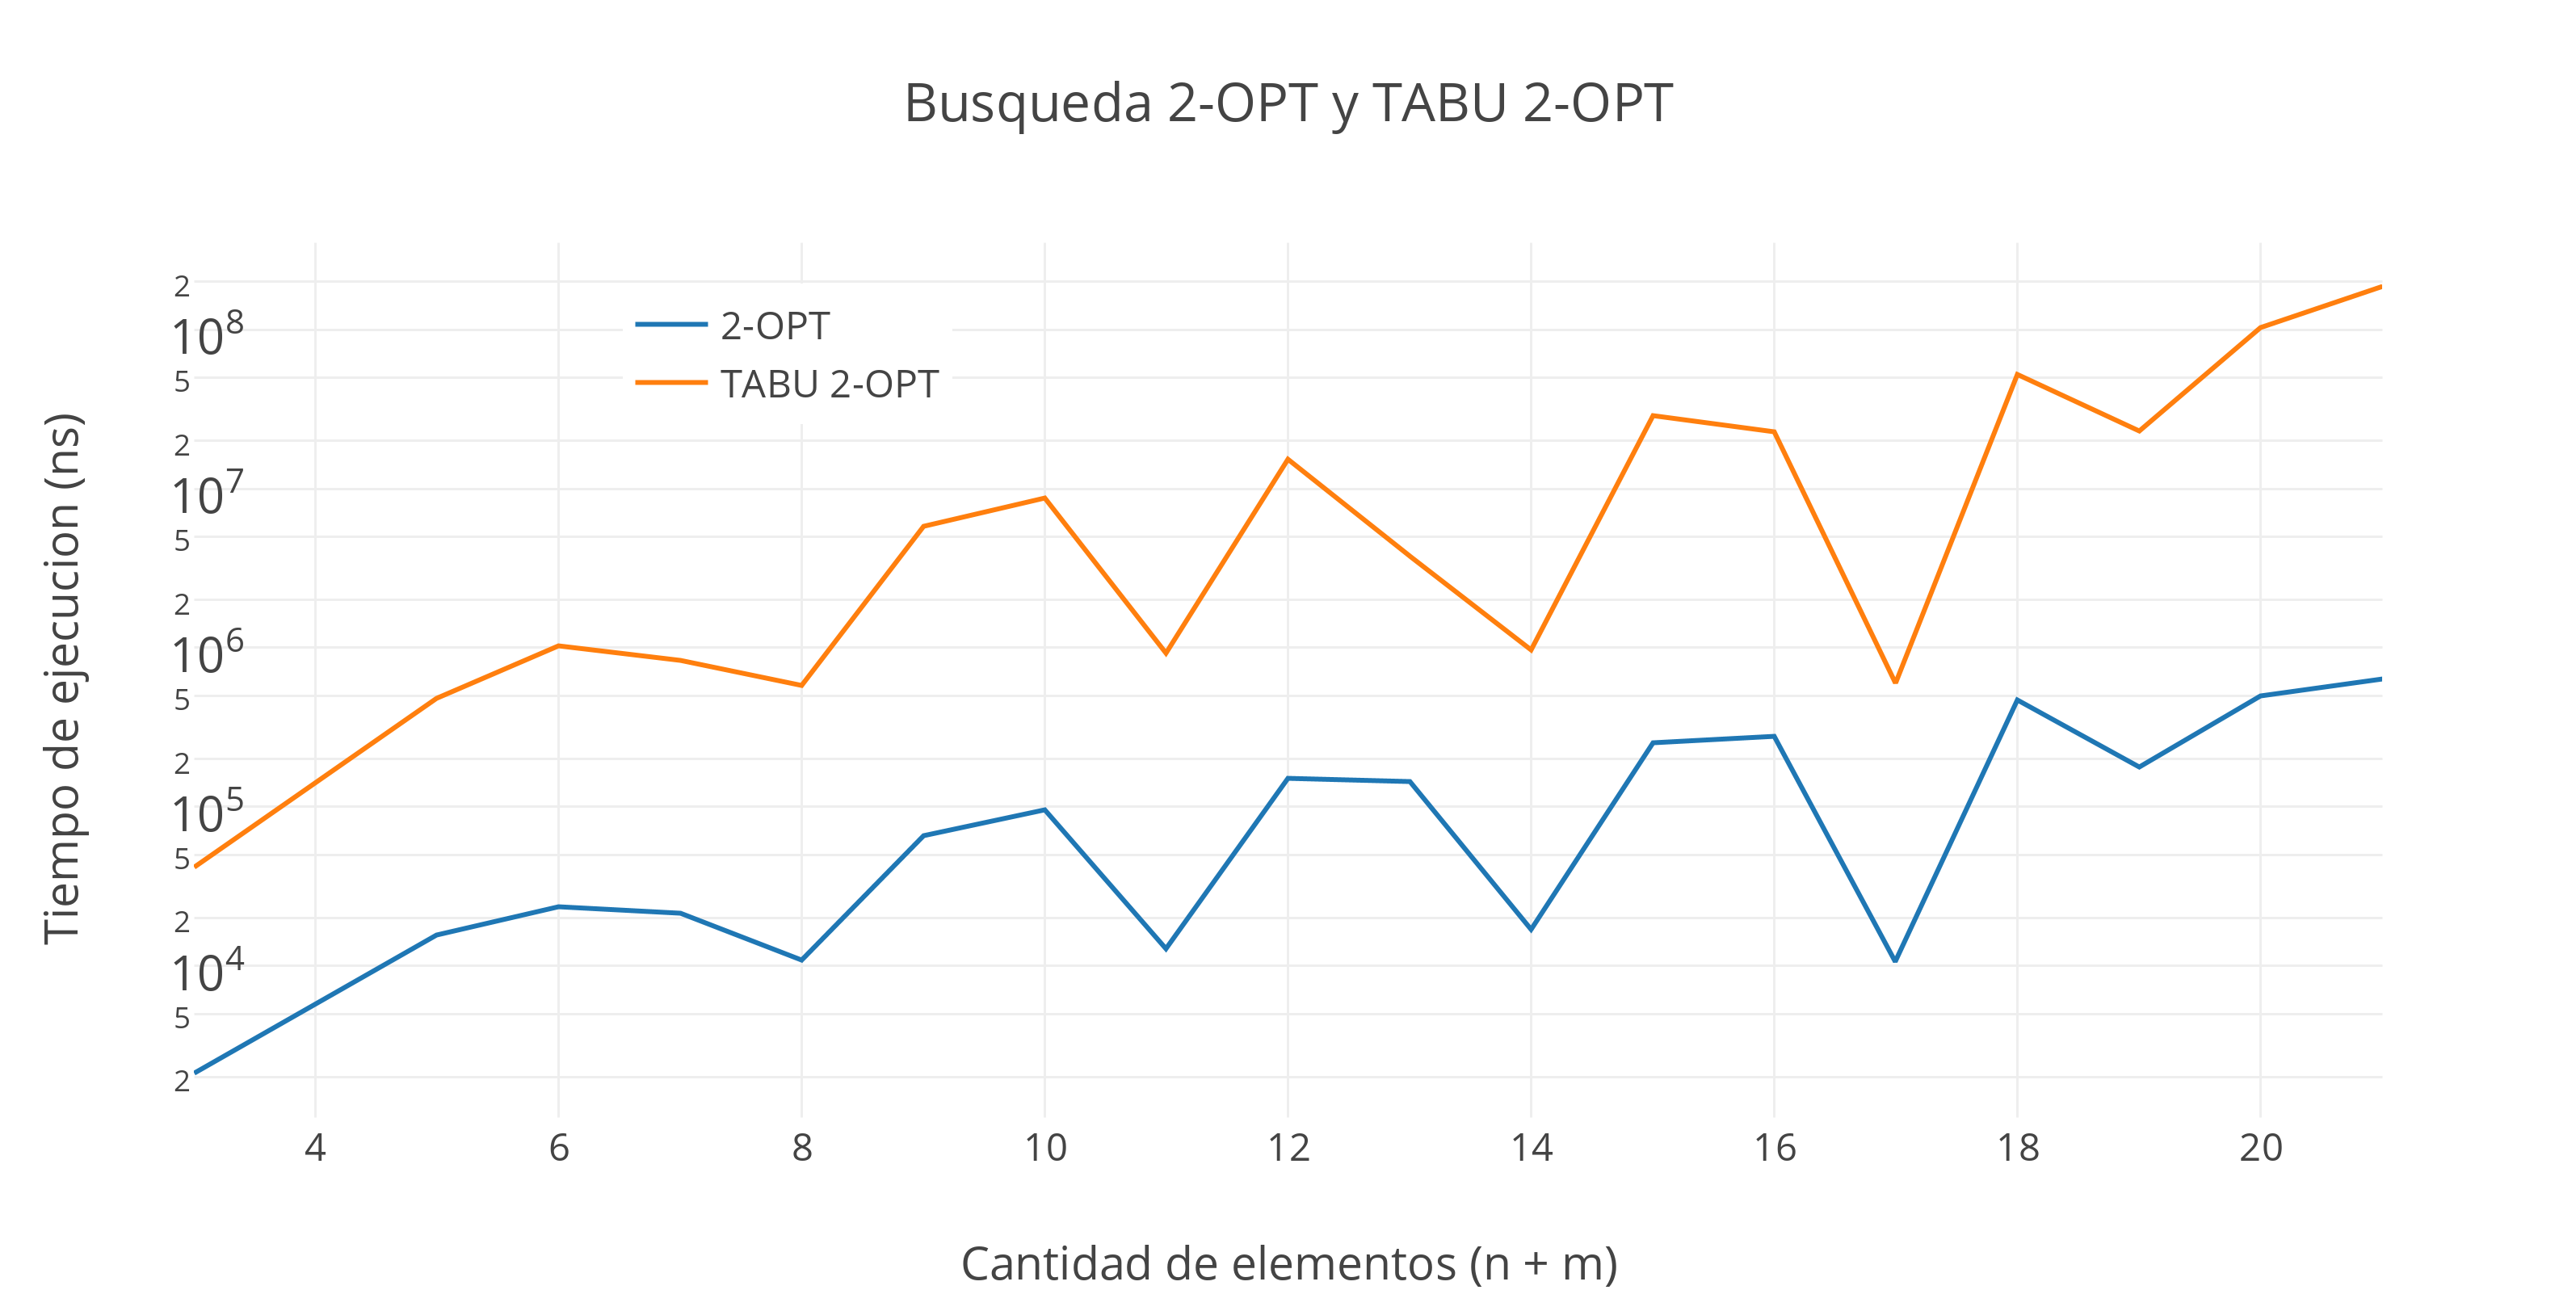
\includegraphics[scale=0.5]{./EJ4/medicionrandom2opt.png}\\
 {            \textit{Gráfico \ 4.8 - 2-OPT vs Tabu 2-OPT sobre Familia 6}}
  \end{center}
  \vspace*{0.3cm}

Luego, para 3-OPT:

\vspace*{0.3cm} \vspace*{0.3cm}
  \begin{center}
 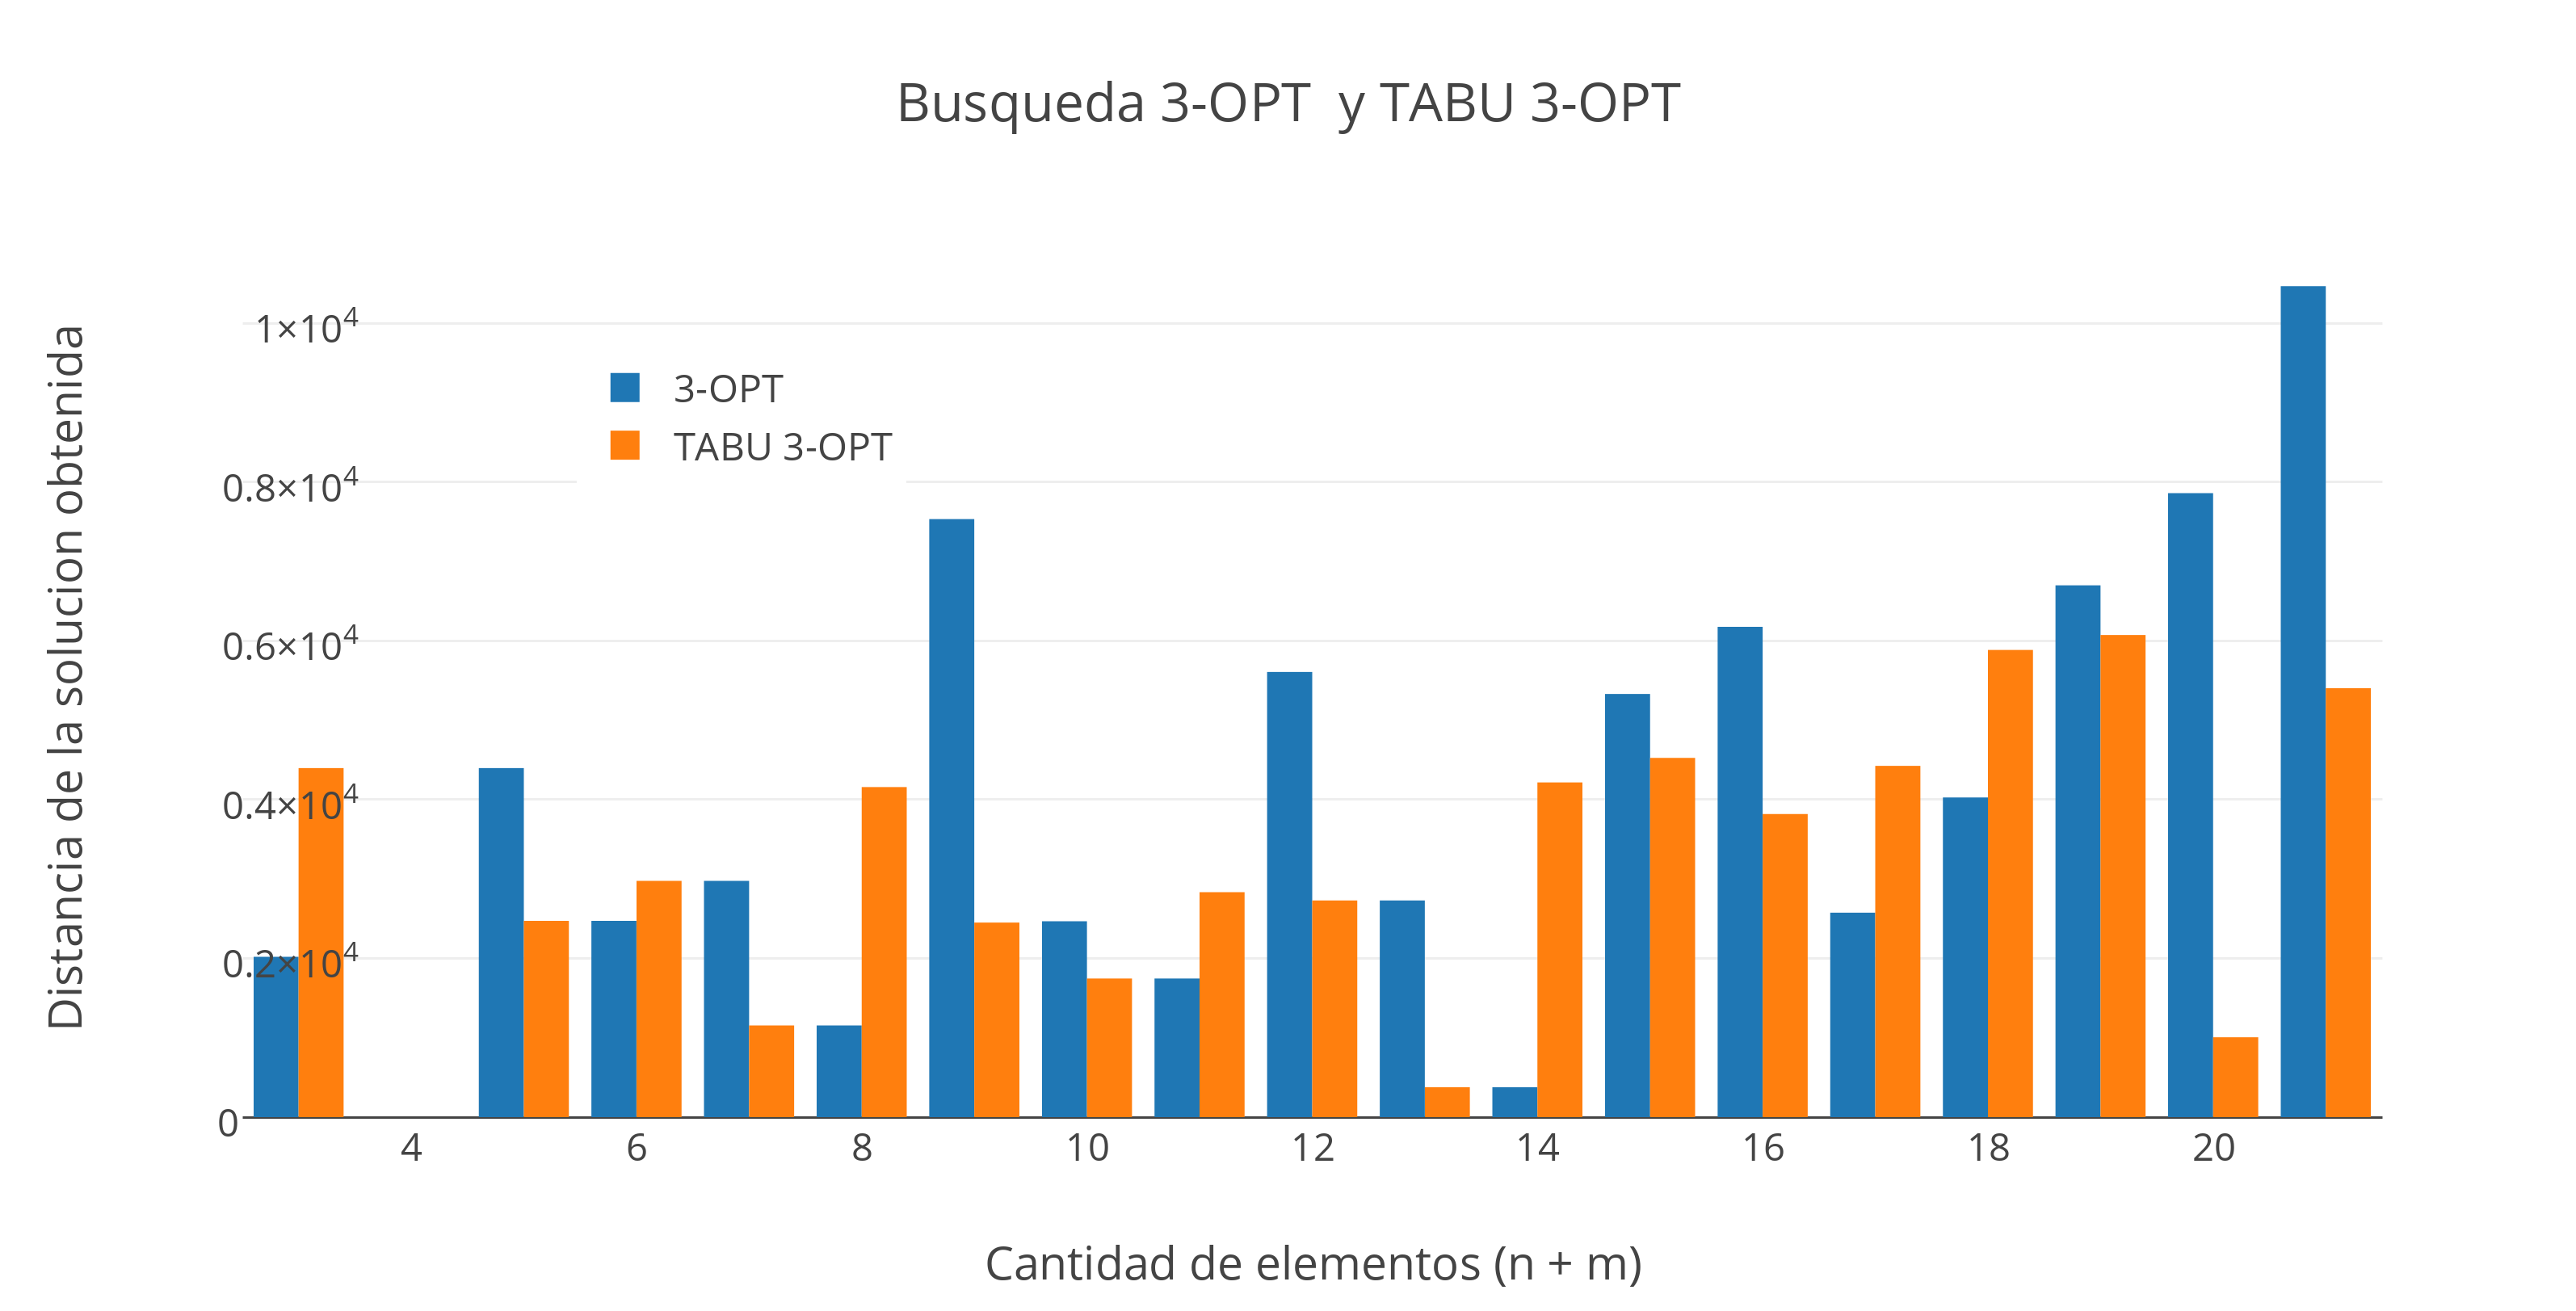
\includegraphics[scale=0.5]{./EJ4/comparativorandom3opt.png}\\
 {            \textit{Gráfico \ 4.9 - 3-OPT vs Tabu 3-OPT sobre Familia 6}}
  \end{center}
  \vspace*{0.3cm}

\vspace*{0.3cm} \vspace*{0.3cm}
  \begin{center}
 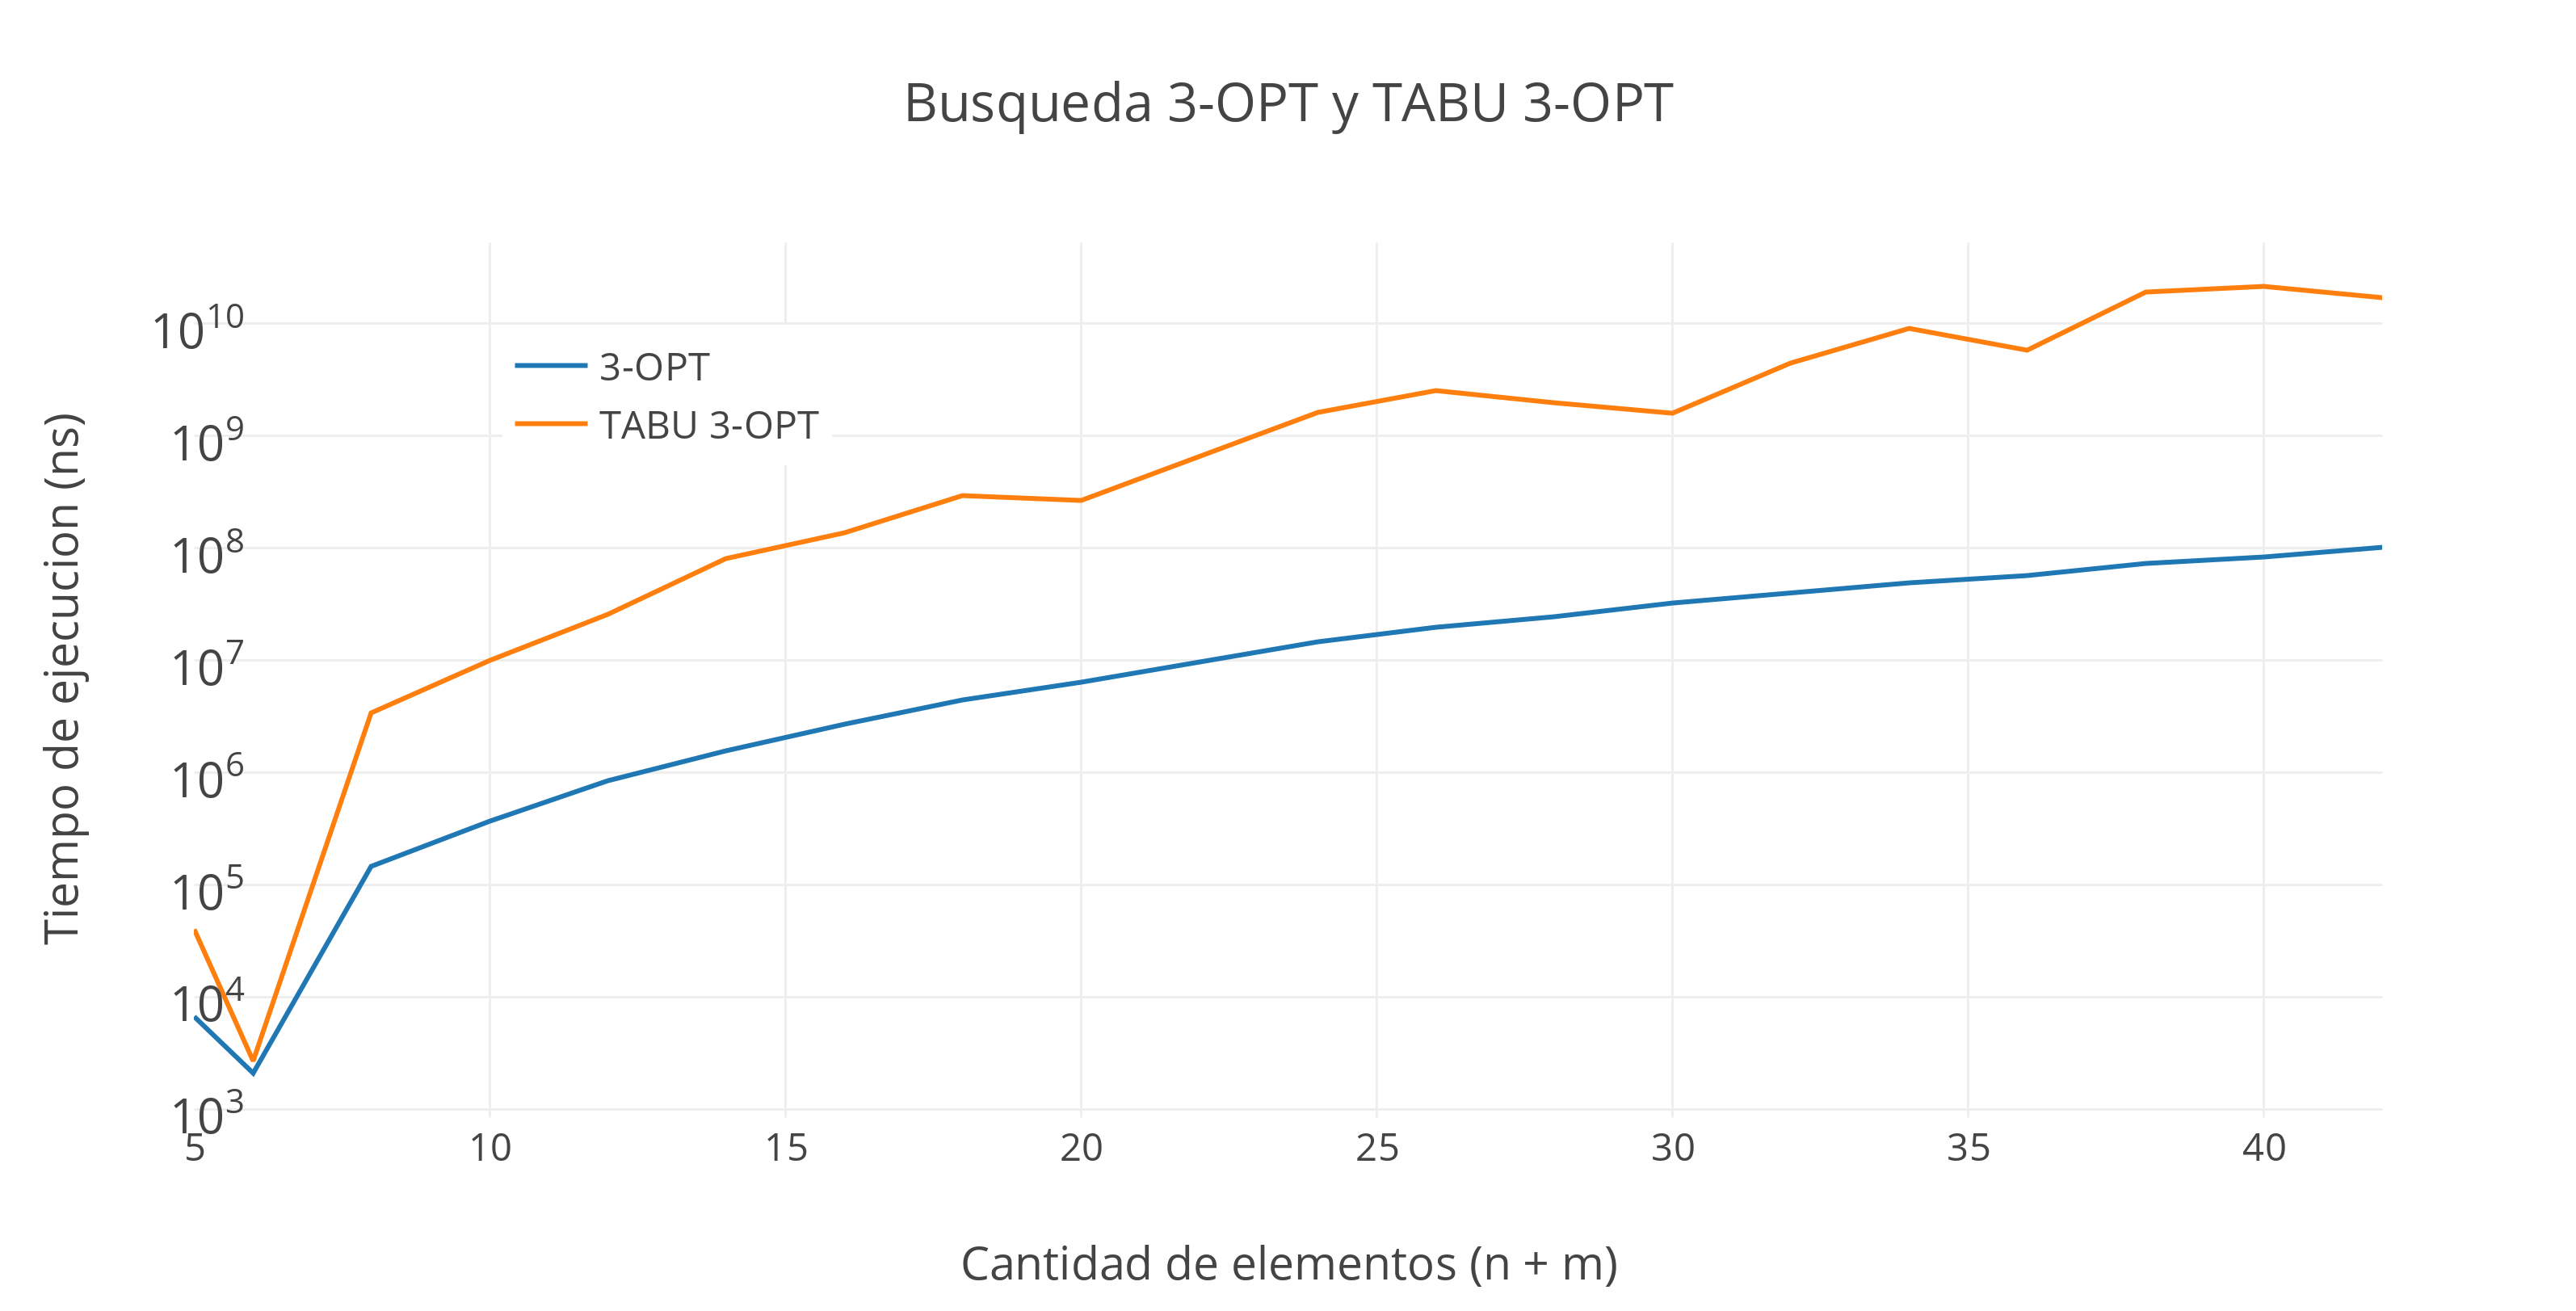
\includegraphics[scale=0.5]{./EJ4/medicionrandom3opt.png}\\
 {            \textit{Gráfico \ 4.10 - 3-OPT vs Tabu 3-OPT sobre Familia 6}}
  \end{center}
  \vspace*{0.3cm}
  
--> OBTENER CONCLUSIONES
  
Comparando las soluciones de cada version de tabú search podemos observar lo siguiente: 

\vspace*{0.3cm} \vspace*{0.3cm}
  \begin{center}
 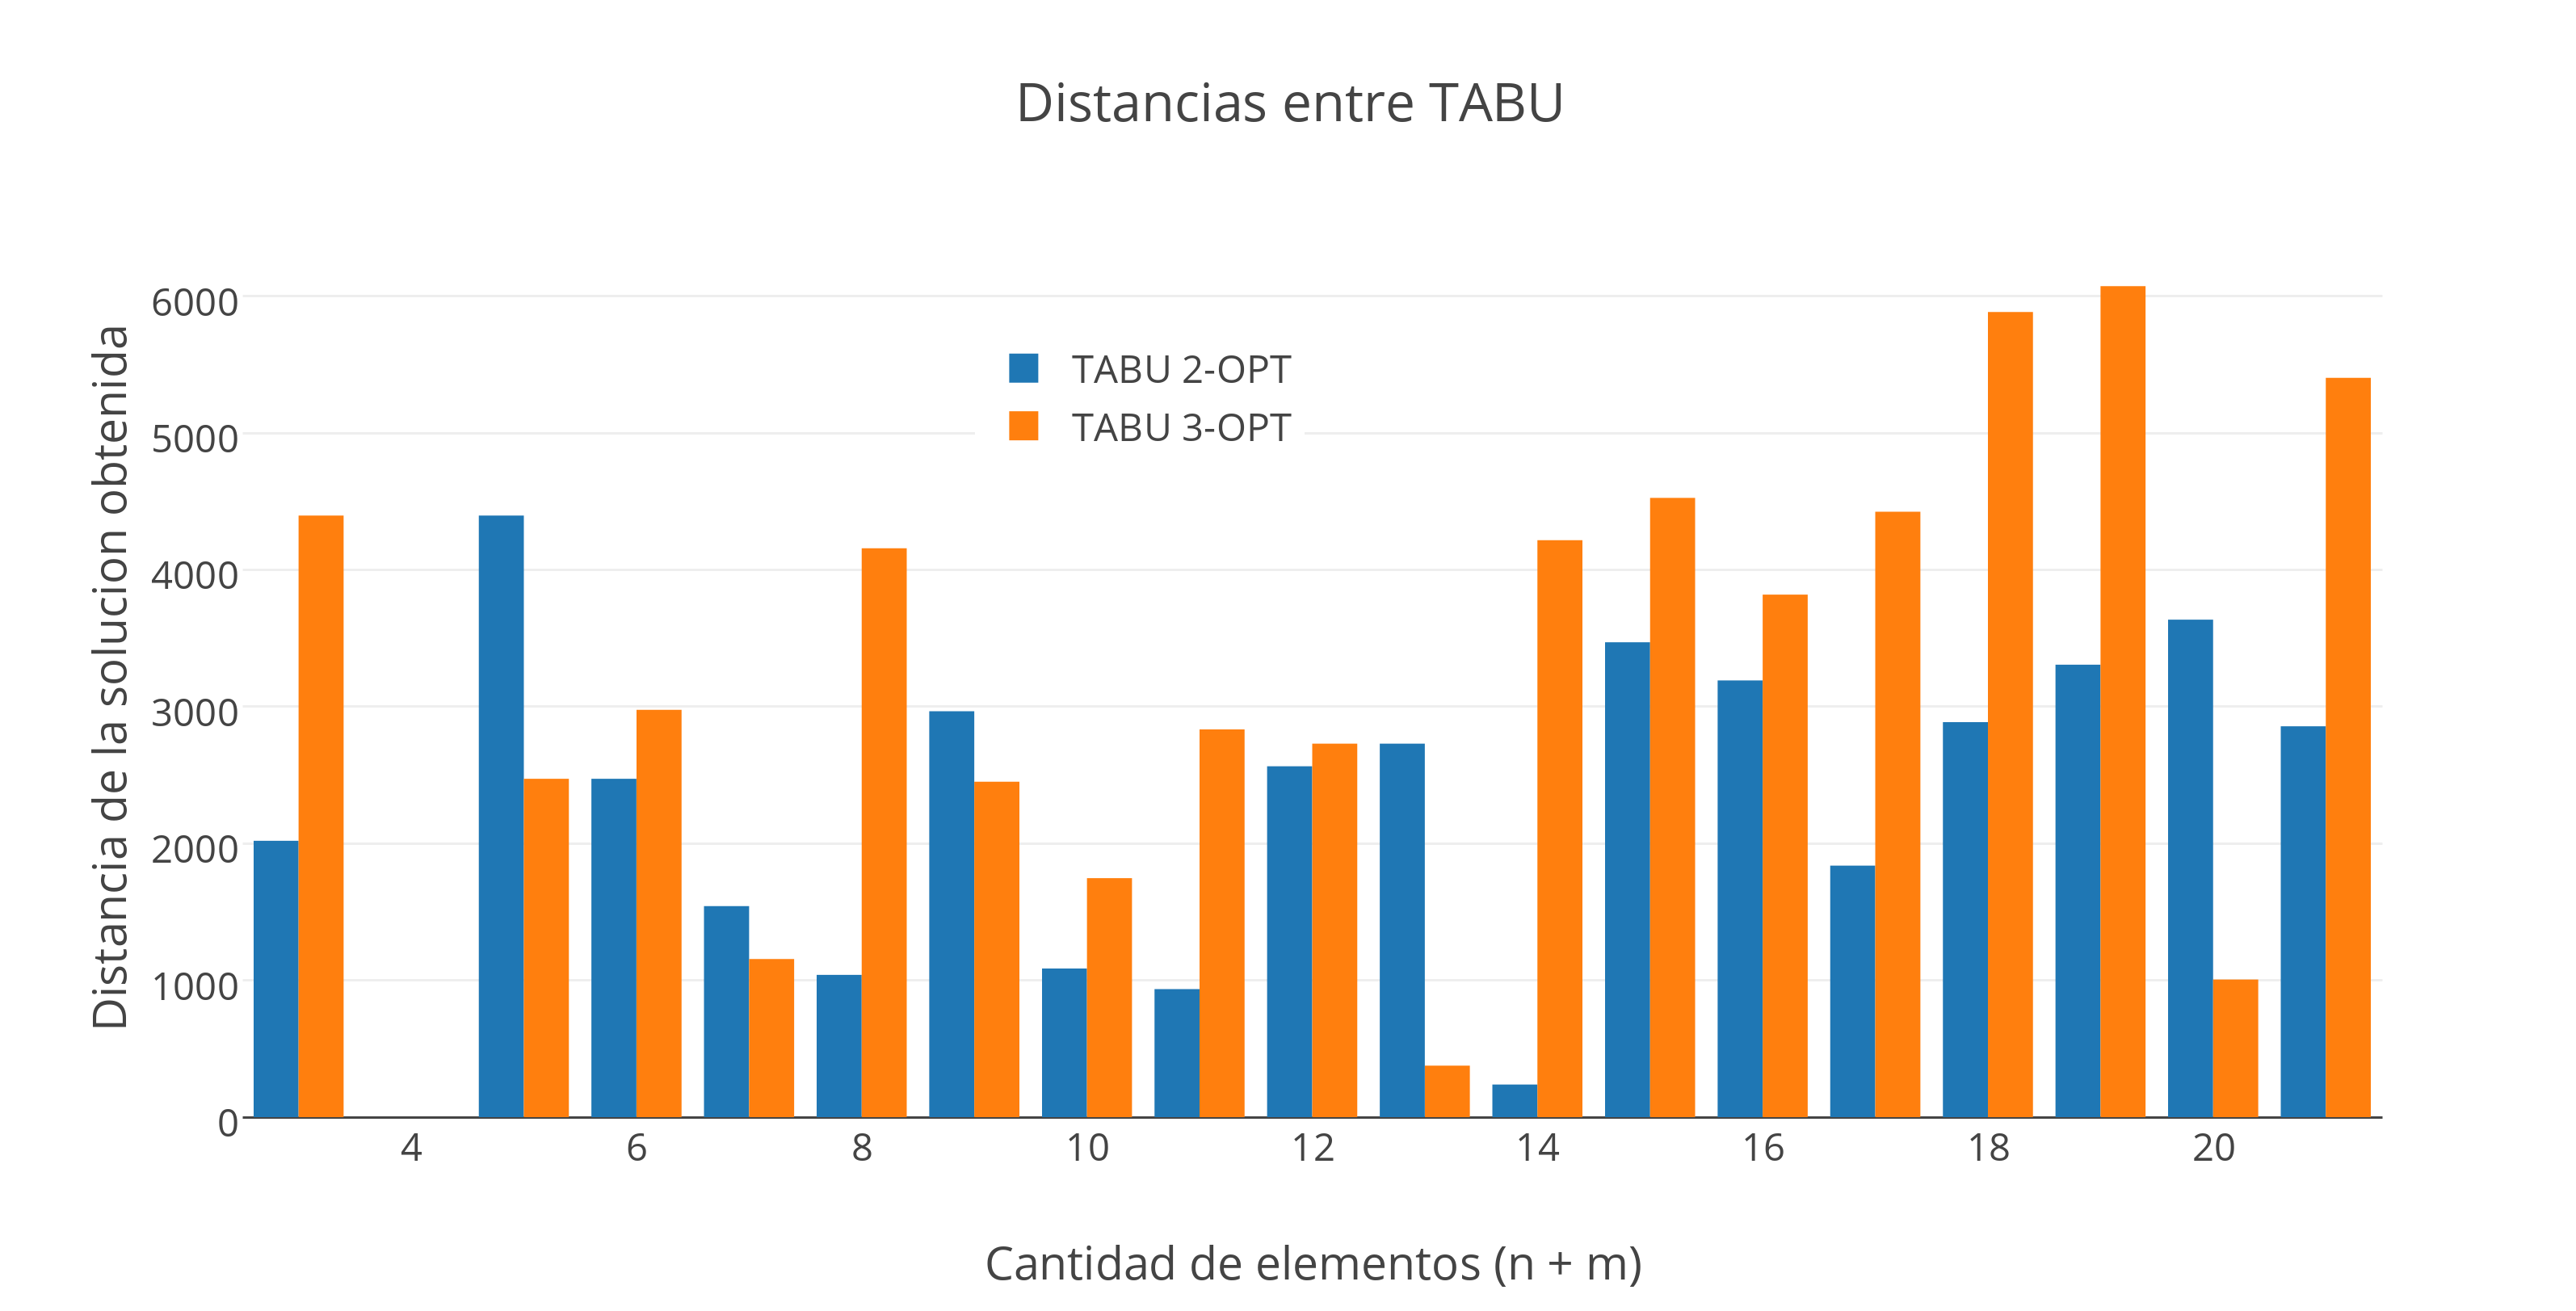
\includegraphics[scale=0.5]{./EJ4/comparativorandom.png}\\
 {            \textit{Gráfico \ 4.11 - Tabu 2-OPT vs Tabu 3-OPT sobre Familia 6}}
  \end{center}
  \vspace*{0.3cm}

\vspace*{0.3cm} \vspace*{0.3cm}
  \begin{center}
 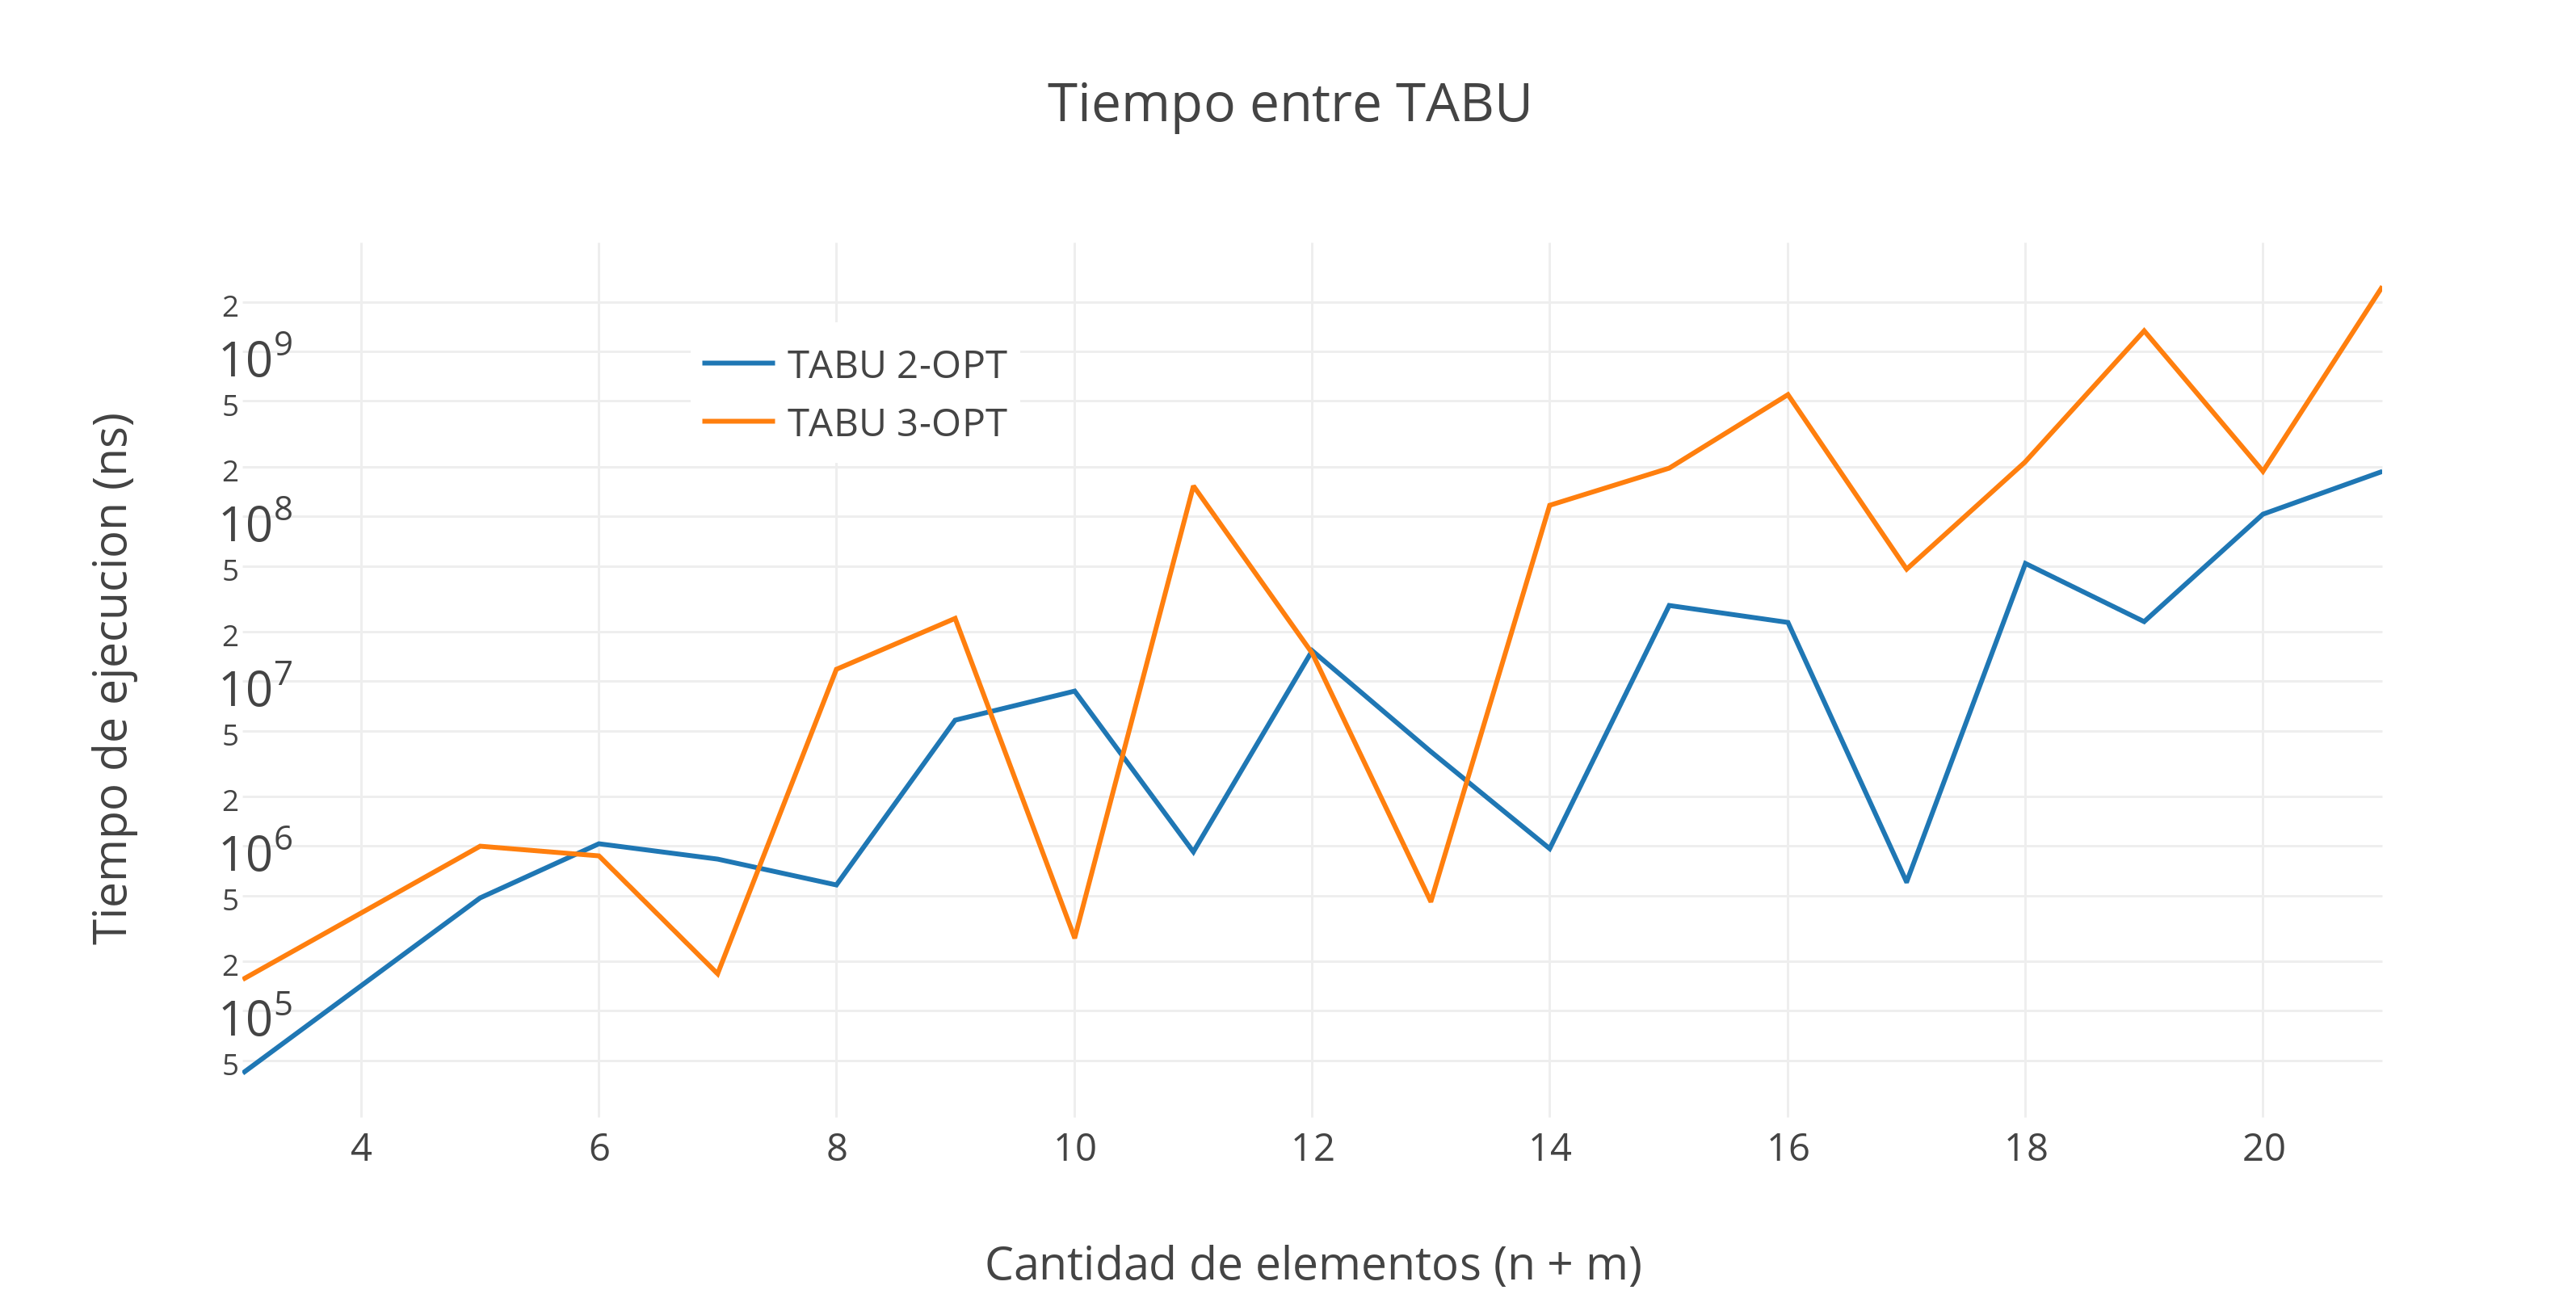
\includegraphics[scale=0.5]{./EJ4/medicionrandom.png}\\
 {            \textit{Gráfico \ 4.12 - Tabu 2-OPT vs Tabu 3-OPT sobre Familia 6}}
  \end{center}
  \vspace*{0.3cm}
  
--> OBTENER CONCLUSIONES

--> OBTENER CONCLUSIONES GENERALES SOBRE ESTOS TESTS: CUAL VERSION DE TABU CONVIENE MAS? EN QUE CASOS CONVIENE HACER BUSQUEDA LOCAL UNICAMENTE?  
  
--> ANALISIS DEL TRADE OFF: sobre la cantidad de iteraciones y la condicion de corte por producirse limite de no mejoras

\vspace*{0.3cm} \vspace*{0.3cm}
  \begin{center}
 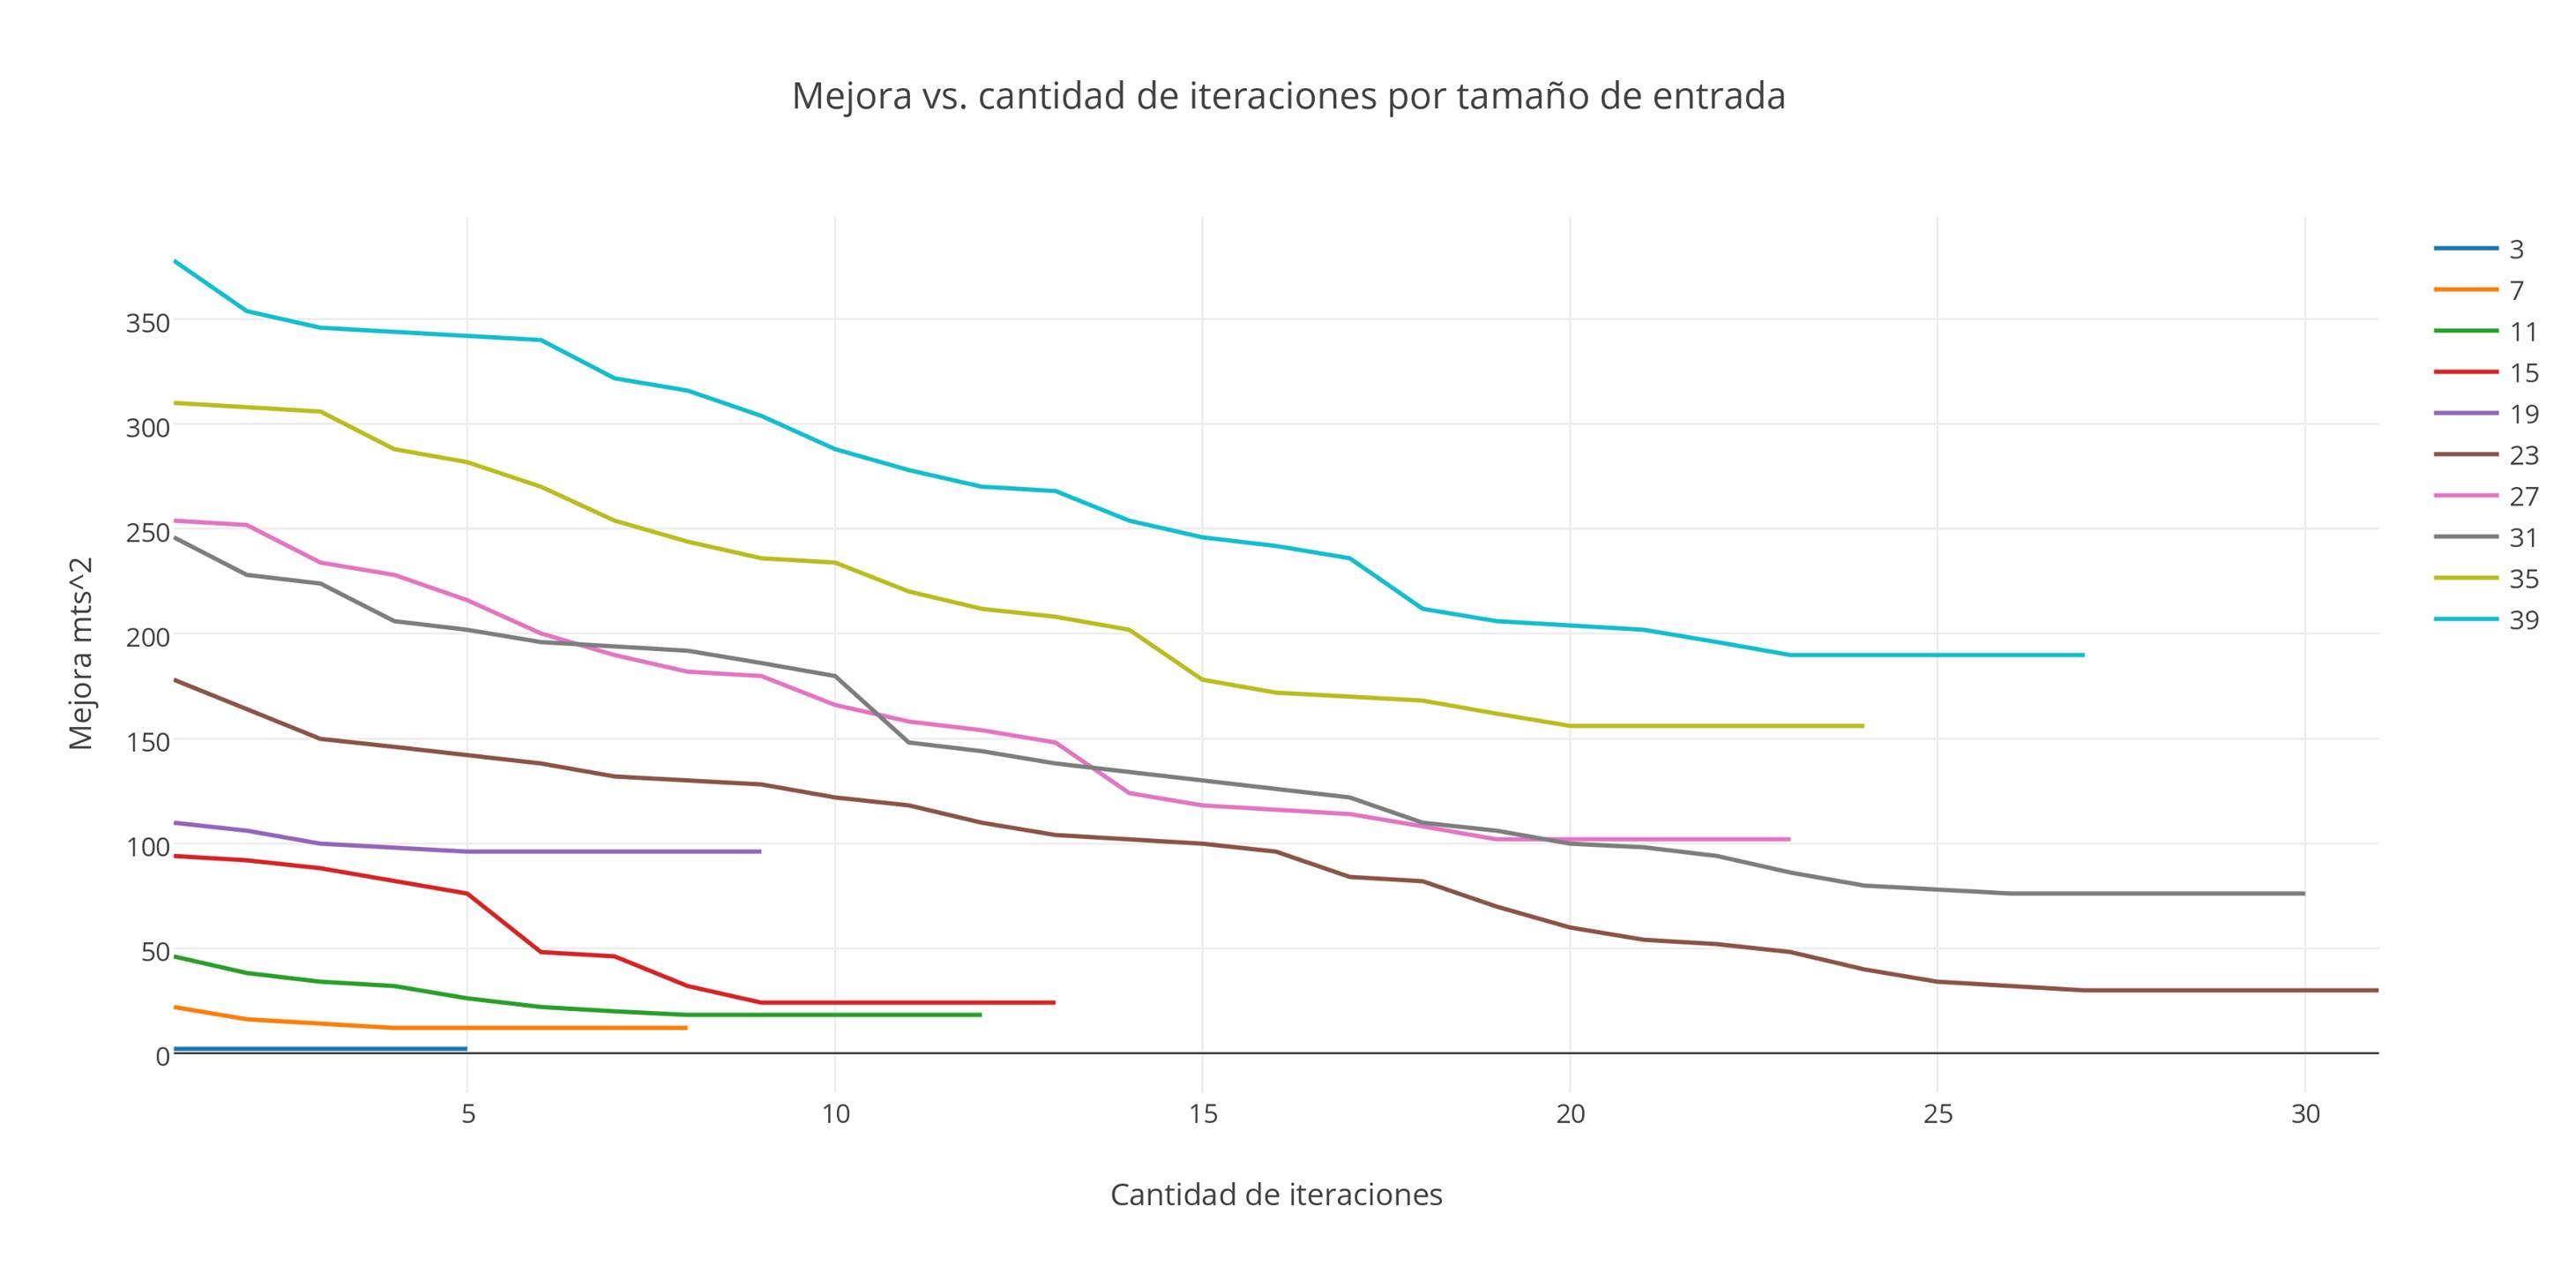
\includegraphics[scale=0.5]{./EJ4/mejora.png}\\
 {            \textit{Gráfico \ 4.12 - Tabu 2-OPT vs Tabu 3-OPT sobre Familia 6}}
  \end{center}
  \vspace*{0.3cm}
  
  \vspace*{0.3cm} \vspace*{0.3cm}
  \begin{center}
 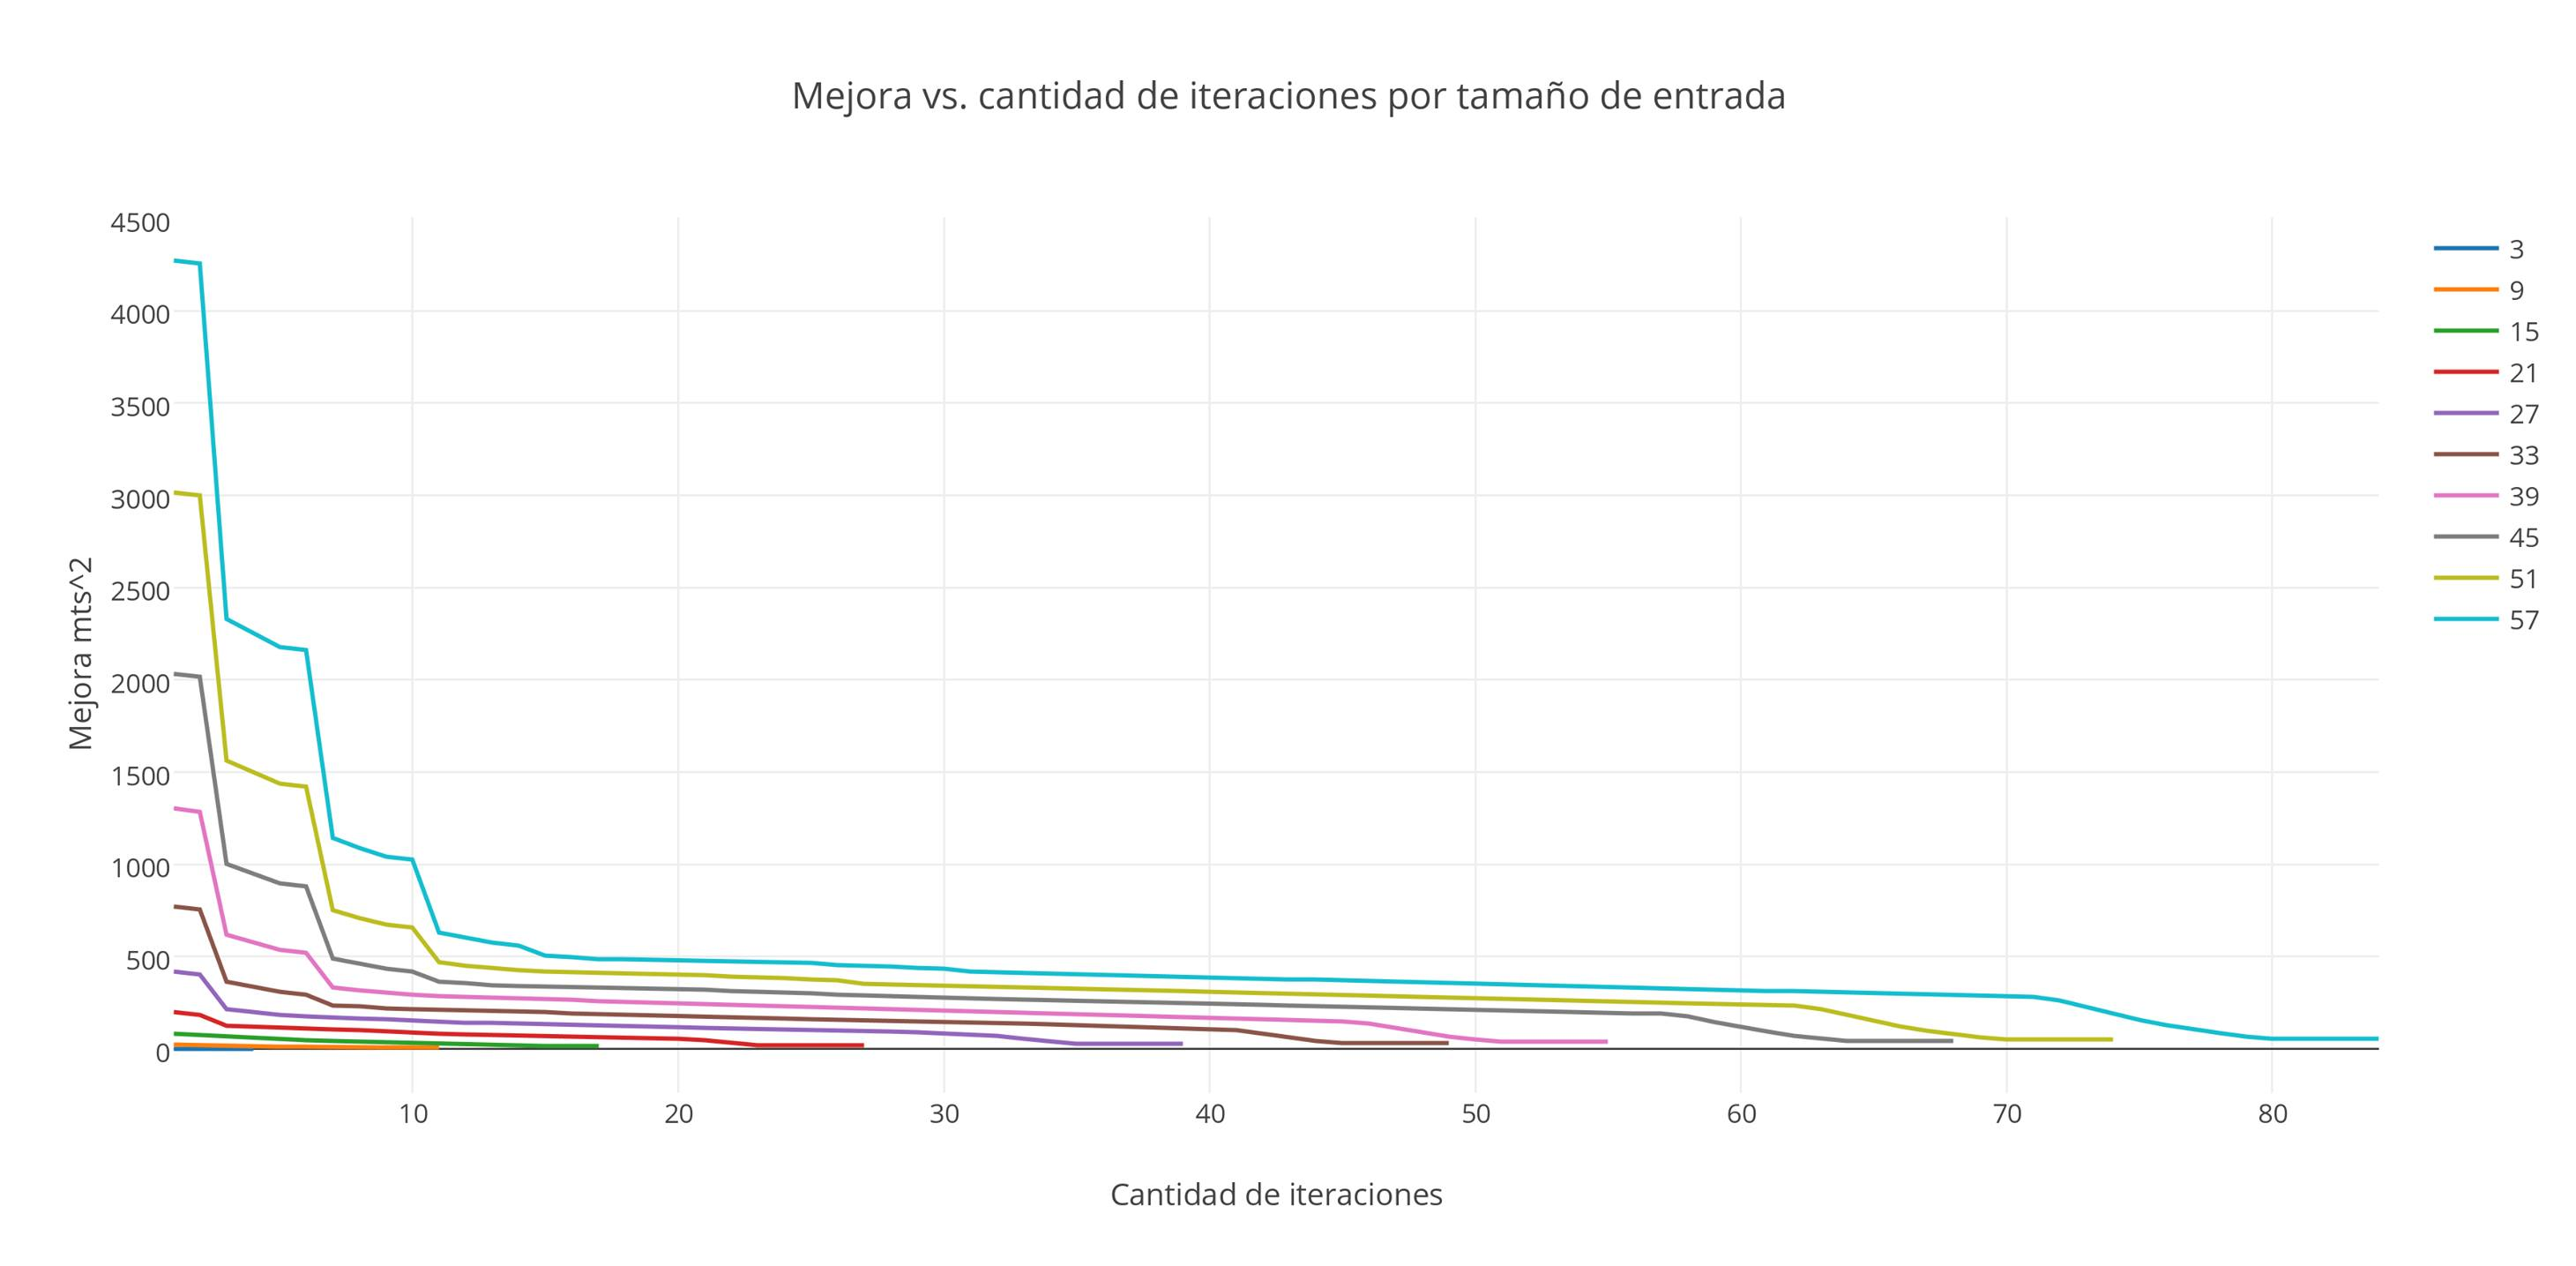
\includegraphics[scale=0.5]{./EJ4/mejora1.png}\\
 {            \textit{Gráfico \ 4.12 - Tabu 2-OPT vs Tabu 3-OPT sobre Familia 6}}
  \end{center}
  \vspace*{0.3cm}
  
  \vspace*{0.3cm} \vspace*{0.3cm}
  \begin{center}
 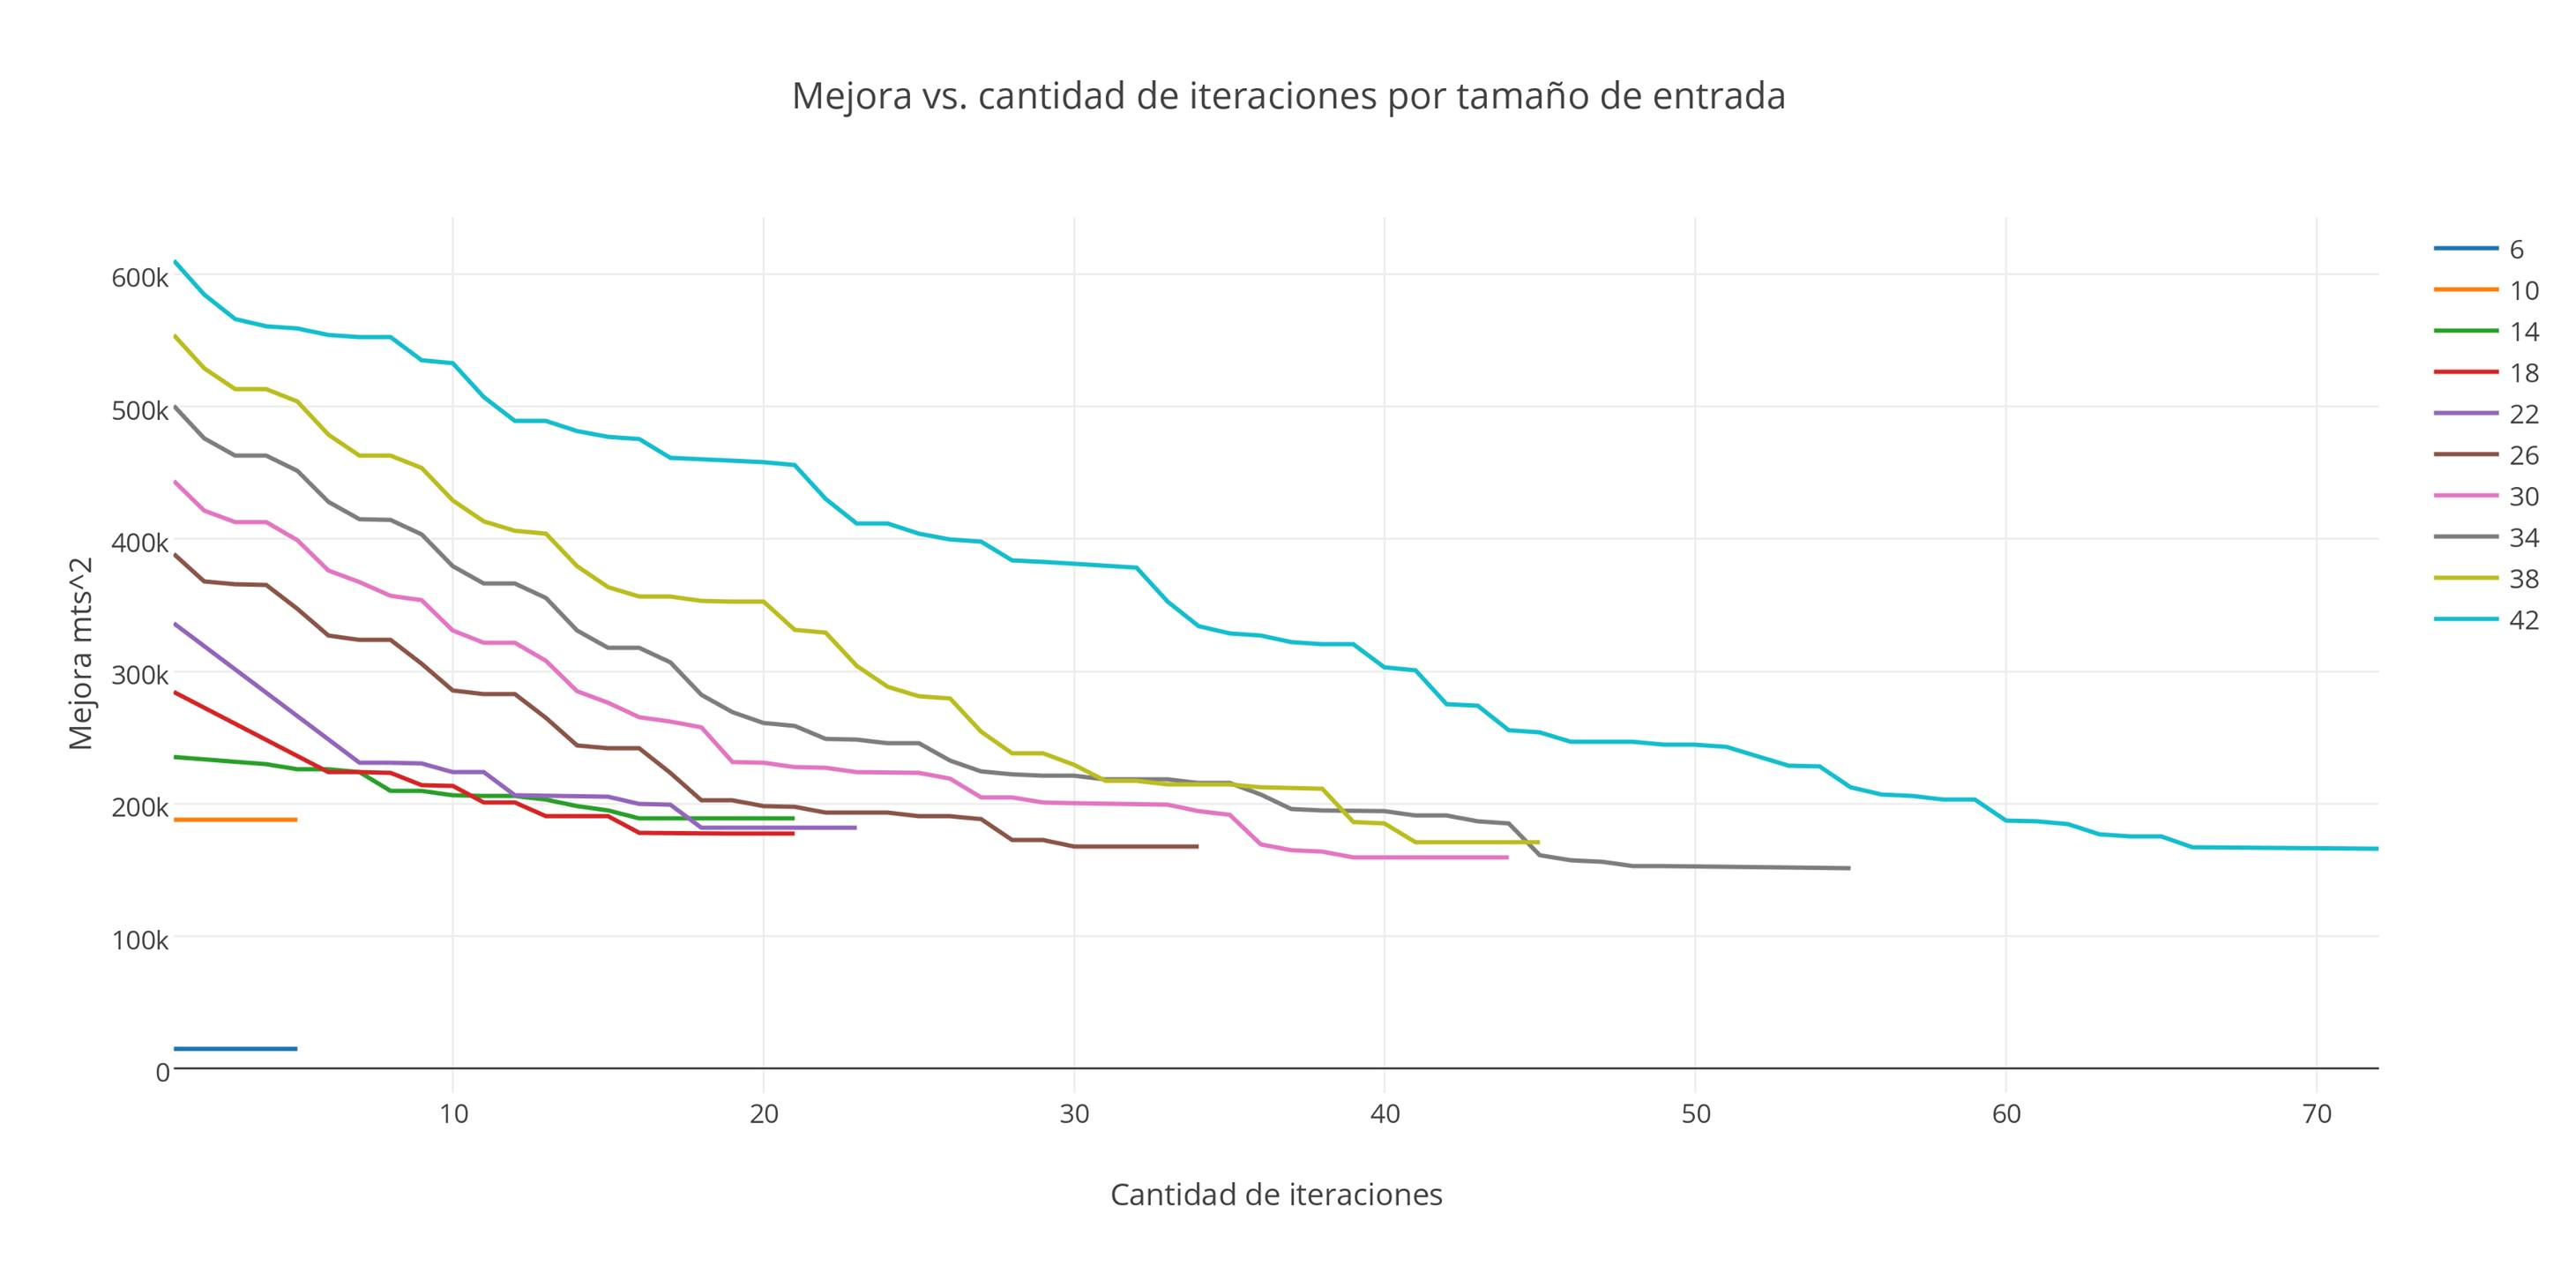
\includegraphics[scale=0.5]{./EJ4/mejora2.png}\\
 {            \textit{Gráfico \ 4.12 - Tabu 2-OPT vs Tabu 3-OPT sobre Familia 6}}
  \end{center}
  \vspace*{0.3cm}
  
--> OBTENER CONCLUSIONES GENERALES: PORQUE SIRVE? CUANDO CONVIENE ? CUANDO NO ? 
  
